\documentclass[11pt,letter]{article}
\usepackage[top=0.65in,bottom=0.9in,left=0.85in,right=0.85in]{geometry}

%\def\baselinestretch{1.25}
\def\baselinestretch{1.0}

\usepackage[greek, english]{babel}
\usepackage{multicol}

%\usepackage[draft]{graphicx}
\usepackage{graphicx}
\usepackage[export]{adjustbox}

\usepackage{setspace}

% The use of the times package forces the use of the type-1 times
% roman font, but the times roman font does not look nice.
% Besides the times roman font still does not print correctly on
% the dopy printer.
%\usepackage{times}


\usepackage{fancyhdr}
\usepackage{amsmath}
\usepackage{bm}
\usepackage{bbold}
\usepackage{parskip}

\newcommand{\bv}[1]{\ensuremath{\bm{#1}}}
\newcommand{\Lc}{\ensuremath{L_{\mathrm{c}}}}
\newcommand{\dsig}[1]{\ensuremath{ \frac{ d\,\sigma_{#1} }{d\,\Omega} }}

\newcommand{\isat}{\ensuremath{I_{\mathrm{sat}}}}
\newcommand{\iisat}{\ensuremath{I_{\mathrm{p}}/I_{\mathrm{sat}}}}
\newcommand{\Iqtof}{\ensuremath{I_{\bv{Q}\infty} }}
\newcommand{\Itof}[1]{\ensuremath{I_{\bv{#1}\infty} }}
\newcommand{\Iq}{\ensuremath{I_{\bv{Q}} }}
\newcommand{\iq}{\ensuremath{i_{\bv{Q}} }}
\newcommand{\Iqma}{\ensuremath{I_{\bv{Q}_{\text{MA}}} }}
\newcommand{\Ima}[1]{\ensuremath{I_{\bv{#1}_{\text{MA}}} }}
\newcommand{\iqma}{\ensuremath{i_{\bv{Q}_{\text{MA}}} }}
\newcommand{\jqma}{\ensuremath{j_{\bv{Q}_{\text{MA}}} }}
\newcommand{\Iqmatof}{\ensuremath{I_{\bv{Q}_{\text{MA}\infty}} }}
\newcommand{\is}{\ensuremath{i_{S}} }
\newcommand{\iqT}{\ensuremath{i_{\bv{Q}_{T}} }}
\newcommand{\ipith}{\ensuremath{i_{\bv{\pi}/\bv{\theta}}}}
\newcommand{\fpith}{\ensuremath{f_{\bv{\pi}/\bv{\theta}}}}
\newcommand{\iT}[1]{\ensuremath{i_{\bv{#1}_{T}} }}
\newcommand{\ima}[1]{\ensuremath{i_{\bv{#1}_{\text{MA}}} }}
\newcommand{\fma}[1]{\ensuremath{f_{\bv{#1}_{\text{MA}}} }}
\newcommand{\jma}[1]{\ensuremath{j_{\bv{#1}_{\text{MA}}} }}


\begin{document}

\section{Scattering of light by an array of atoms}

In our experiment we observe the scattering of photons from atoms confined in
an optical lattice, here we treat this situation by first obtaining  the field
scattered from a single atom and then summing the field contributions from all
the atoms coherently at the location of our detector.  The main goal of this
document is to find the connection between the intensity that we measure in our
cameras and the spin structure factor as calculated by the theorists in our
collaboration.  

\subsection{Electric field and intensity due to a single atom}

To calculate the scattered field, one uses the source-field expression, which
relates the radiated field to the emitting dipole moment, this is derived in
the standard textbooks~\cite{loudon2000quantum,cohen1998atom}.  The field at
the position of the detector $\bv{r}_{D}$ is given by
\begin{equation} 
    E^{(+)}( \bv{r}_{D}, t) = 
    \eta e^{- i \omega_{L} ( t -r_{D}/c) } 
    S_{-}\left(t - \frac{ r_{D} }{c} \right)
    \label{eq:source-field} 
\end{equation} where $\eta$
is a proportionality factor that we will address later on.  The time-averaged
intensity at the detector is 
\begin{equation}
\label{eq:Idef}
\begin{split}
\langle I (t) \rangle = & 
    \langle E^{(-)}(\bv{r}_{D}, t) E^{(+)}(\bv{r}_{D}, t) \rangle \\
   = & |\eta|^{2} \langle S_{+}(t-r_{D}/c)S_{-}(t-r_{D}/c) \rangle  \\
\end{split}
\end{equation}
In the steady state $\langle S_{+}(t) S_{-}(t) \rangle$ does not depend on $t$,
so
\begin{equation}
\begin{split} 
\langle I (t) \rangle  
   = & |\eta|^{2} \langle S_{+}S_{-} \rangle \\
   = & |\eta|^{2} \rho_{ee}  
\end{split} 
\end{equation}
We can write the $S_{\pm}$ operators of the atoms as 
\begin{equation} 
    S_{\pm} = \langle S_{\pm} \rangle + \delta S_{\pm} 
\end{equation}
which defines the difference, $\delta S$, between $S_{\pm}$ and its average
value.   Writing $S_{\pm}$ this way allows us to distinguish between two
components in the radiated light:  the radiation of the average dipole $\langle
S_{\pm}\rangle$ which is the radiation of a classical oscillating dipole with a
phase that is well defined relative to the incident laser field, and the
radiation from the $\delta S_{\pm}$ component which does not have a phase that
is well defined relative to the incident field because it comes form the
fluctuating part of the atomic dipole.  The intensity is then a sum of coherent
and incoherent parts 
\begin{equation} 
I  = \eta^{2} \langle S_{+}\rangle \langle S_{-} \rangle 
   + \eta^{2} \langle \delta S_{+} \delta S_{-} \rangle 
\end{equation}
where we have used the fact that by definition $\langle \delta S_{\pm}
\rangle = 0$. The first and second terms of this equation are the coherent
and incoherent intensity which can be calculated by using the
steady-state solutions to the optical Bloch equations:
\begin{gather} 
    \langle S_{\pm} \rangle =  u \pm i v  \\
    u =  \frac{ \Delta }{ \Gamma  \sqrt{ I_{\mathrm{p}} / I_{\mathrm{sat}}} } 
         \frac{s}{ 1 + s } \\
    v =  \frac{ 1 } { 2 \sqrt{ I_{\mathrm{p}} / I_{\mathrm{sat}}} } 
         \frac{s}{1+s} \\
\end{gather}
where $s$ is the saturation parameter for an incident probe with intensity
$I_{\mathrm{p}}$:
\begin{equation}
s = \frac{ 2  \iisat } { 1 + 4(\Delta/\Gamma)^{2} } 
  =  \frac{ s_{0} } { 1 + 4(\Delta/\Gamma)^{2} }
\end{equation}
and we have defined $s_{0} = 2 \iisat$. 
The coherent and incoherent intensities are
\begin{equation}
\begin{split} 
    \frac{1}{\eta^{2}}  I_{\mathrm{coh}} = &
        \frac{1}{2} \frac{s}{(1+s)^{2} } 
      = \rho_{ee}  \frac{1}{1+s} \\
    \frac{1}{\eta^{2}}  I_{\mathrm{incoh}}  = & 
        \langle S_{+}S_{-} \rangle - \langle S_{+} \rangle \langle S_{-} \rangle
      = \frac{1}{2} \frac{s^{2}}{(1+s)^{2}} = \rho_{ee} \frac{s}{1+s}
 \label{eq:coh-incoh} 
\end{split}
\end{equation}
Note that if we add up coherent and incoherent part we get the familiar result
$I=\eta^{2} \rho_{ee}$, where the total intensity is simply proportional to the
population of the excited state.


\subsection{Scattering cross-section}

Now we will turn onto the evaluation of $\eta$, the proportionality factor
between the field and the emitting dipole.  Knowledge of $\eta$ will allow us
to sum coherently the field from a collection of atoms. 

We start by considering the  transition matrix element between the following
initial and final states of the atom+photon system: 
\begin{equation}
\begin{split}
    | \varphi_{i} \rangle = & | g ; \bv{k}\bv{\varepsilon} \rangle \\
    | \varphi_{f} \rangle = & | g' ; \bv{k}'\bv{\varepsilon}' \rangle \\
\end{split}
\end{equation}
These states represent the absorption and re-emission of a single photon by the
atom, with two possibly different initial and final photon states, and two
possibly different initial and final atom ground states.
 
The transition rate to from $i\rightarrow f$ is given by 
\begin{equation}
    \label{eq:transitionRate}
    w_{fi} = \frac{2\pi}{\hbar} | \mathcal{T}_{fi} |^{2} \delta(E_{f}-E_{i})
\end{equation}
Where we use the notation in~\cite{cohen1998atom} (see Exercise~5 on pg. 530),
and $\mathcal{T}_{fi}$ is given by
\begin{equation}
    \mathcal{T}_{fi} = \frac{  
        \langle g; \bv{k}'\bv{\varepsilon}'| H_{I}' | e; 0 \rangle 
        \langle e; 0 | H_{I}' | g; \bv{k}\bv{\varepsilon} \rangle }
        { \hbar\omega - \hbar\omega_{0} + i\hbar (\Gamma/2 ) }
\end{equation} 
where $H_{I}'$ is the interaction Hamiltonian
\begin{equation}
    H_{I}' = -\bv{d} \cdot \bv{E}_{\perp} ( \bv{r} ) 
\end{equation}
and\footnote{Notice that the presence of $\epsilon_{0}$ reveals that we are
using SI units, following the treatment in~\cite{cohen1998atom}.}
\begin{equation}
    \bv{E}_{\perp}(\bv{r}) = i \sum_{j} 
        \left[ \frac{ \hbar \omega_{j} }{ 2\varepsilon_{0} L^{3}}  \right]^{1/2}
        \left( \hat{a}_{j}\bv{\varepsilon}_{j} e^{i\bv{k}_{j}\cdot\bv{r}} 
              - \hat{a}_{j}^{+}\bv{\varepsilon}_{j}^{*} e^{-i\bv{k}_{j}
                \cdot\bv{r}} 
        \right)
\end{equation}
Notice that there is an intermediate excited state $|e;0\rangle$, since the
absorption-emission event is a second order process.

Using the expressions for $H_{I}'$ and $\bv{E}_{\perp}(\bv{r})$ we obtain for
the matrix element 
\begin{equation}
   \langle e; 0 | H_{I}' | g; \bv{k}\bv{\varepsilon} \rangle = 
       -i \sqrt{ \frac{ \hbar \omega }{2 \varepsilon_{0} L^{3} }} 
      \langle e | (\bv{d} \cdot \bv{\varepsilon}^{*} ) 
       e^{-i\bv{k}\cdot\bv{r}}| g \rangle
\end{equation}
At this point the textbook treatment usually assumes that the atom is at the
origin and that the size of the atom wavefunction is very small compared to
$|\bv{k}|^{-1}$, and so the exponential inside the matrix element typically
does not show up.  In our case the atom is in a lattice site and its center of
mass state is one of the harmonic oscillator states of a lattice well, which is
large enough that the exponential term cannot be neglected.  
 
The states $|e\rangle$ and $|g\rangle$ include the center of mass and internal
states of the atom.  We separate the center of mass part, and keep the labels
$e$, $g$ for the internal states. Also, we denote the center of mass initial
and final states as $| u \rangle$ and $|u'\rangle$ respectively, and the center
of mass state of the intermediate excited state as $| v\rangle$, we have
\begin{equation}
   \langle e; 0 | H_{I}' | g; \bv{k}\bv{\varepsilon} \rangle = 
       -i \sqrt{ \frac{ \hbar \omega }{2 \varepsilon_{0} L^{3} }} 
      \langle e | \bv{d} \cdot \bv{\varepsilon}^{*} | g \rangle 
      \langle v | e^{-i\bv{k}\cdot\bv{r}} | u \rangle
\end{equation}
and similarly
\begin{equation}
   \langle g; \bv{k}'\bv{\varepsilon}' | H_{I}' | e; 0\rangle = 
       i \sqrt{ \frac{ \hbar \omega' }{2 \varepsilon_{0} L^{3} }} 
      \langle g | \bv{d} \cdot \bv{\varepsilon}' | e \rangle 
      \langle u' | e^{i\bv{k}'\cdot\bv{r}} | v \rangle
\end{equation}
This gives for the matrix element
\begin{equation}
    \mathcal{T}_{fi} = \sum_{v} \frac{\sqrt{\omega \omega'}}
                                     {2\varepsilon_{0} L^{3}}
    \frac{ 
      \langle g | \bv{d} \cdot \bv{\varepsilon}' | e \rangle 
      \langle e | \bv{d} \cdot \bv{\varepsilon}^{*} | g \rangle 
      \langle u'| e^{i\bv{k}'\cdot\bv{r}} | v \rangle 
      \langle v | e^{-i\bv{k}\cdot\bv{r}} | u  \rangle
       }
        { \omega - \omega_{0} + i (\Gamma/2 ) }
\end{equation}
where we have summed over all possible intermediate center of mass states.
Note that the sum can be taken out using the closure relation
$\sum_{v}|v\rangle\langle v| = \mathbb{1}$. 
%We note here that the phase factors $i\bv{k}\cdot\bv{r}$ that appear due to
%the center of mass motion of the atom are uncorrelated.   This comes out that
%way because the scattering of a photon is second order: first the photon gets
%absorbed and then it gets reemitted at a later time.   In neutron scattering
%for example, the scattering process is first order, represented by a contact
%interaction between the neutron and the nuclei in the crystal,  In this case
%the phase factor due to the center of mass motion shows up as \begin{equation}
%\langle  e^{i (\bv{k}'-\bv{k}) \cdot \bv{r}} \rangle_{\mathrm{CM}}
%\end{equation} The norm squared of this term is the Debye-Waller factor.   It
%is necessary to consider if the uncorrelated expectation values that appear in
%the second order photon scattering are correct.  To this effect one needs to
%consider the time between absorption and emission processes which is on the
%order of $\Gamma$, the linewidth of the excited state.   This is much larger
%that the typical harmonic oscillator frequency in a lattice site, which is
%about 400 kHz for a lithium atom in a 50 recoil lattice.   With this in mind
%we may think about photon scattering as an effectively first order process
%(scattering and emission happen much quicker than the atom's center of mass
%can move)  and we may take the liberty of writing the transition matrix
%element which includes the center of mass motion as \begin{equation}
%\begin{split} \langle \mathcal{T}_{fi} \rangle_{\mathrm{CM}} = & \left \langle
%\frac{  \langle g; \bv{k}'\bv{\varepsilon}'| H_{I}' | e; 0 \rangle \langle b;
%0 | H_{I}' | g; \bv{k}\bv{\varepsilon} \rangle } { \hbar\omega -
%\hbar\omega_{0} + i\hbar (\Gamma/2 ) } \right \rangle _{\mathrm{CM}} \\ =&
%\frac{\sqrt{\omega \omega'}}{2\varepsilon_{0} L^{3}} \frac{ \langle g | \bv{d}
%\cdot \bv{\varepsilon}' | e \rangle \langle e | \bv{d} \cdot \bv{\varepsilon}
%| g \rangle \langle  e^{i(\bv{k}'-\bv{k}) \cdot\bv{r}} \rangle_{\mathrm{CM}} }
%{ \omega - \omega_{0} + i (\Gamma/2 ) } \end{split} \end{equation} where the
%more famliar Debye-Waller factor shows up.  

In our experiment we are driving a sigma-minus transition so we can consider
only the projection of $\bv{d}$ onto $\bv{\varepsilon}_{-}$ 
\begin{equation}
     \langle e | \bv{d} \cdot \bv{\varepsilon}^{*} | g \rangle  \equiv
     d_{-} (\bv{\varepsilon}_{-}  \cdot \bv{\varepsilon}^{*} )
\end{equation} 
which leads to 
\begin{equation}
    \mathcal{T}_{fi}  = 
    \frac{\sqrt{\omega \omega'}}{2\varepsilon_{0} L^{3}}
    \frac{ |d_{-}|^{2}  (\bv{\varepsilon}_{+}\cdot \bv{\varepsilon}' )
                       (\bv{\varepsilon}^{*}\cdot \bv{\varepsilon}_{-} )}
        { \omega - \omega_{0} + i (\Gamma/2 ) }
      \langle u' | e^{i(\bv{k}'-\bv{k}) \cdot\bv{r}} | u  \rangle
\end{equation}
We use the relation between $|d_{-}|^{2}$ and the linewidth of the transition
\begin{equation} 
    |d_{-}|^{2} =  3\pi \varepsilon_{0} \hbar
  \left( \frac{c}{\omega_{0}} \right)^{3}  \Gamma
\end{equation}
and also the approximation $\omega' \approx \omega \approx \omega_{0}$ for the
square root in the denominator to obtain
\begin{equation}
    \mathcal{T}_{fi} =
    \frac{ 3 } {k^{2}} 
    \frac{ \pi \hbar c } {  L^{3} } 
        (\bv{\varepsilon}_{+}\cdot \bv{\varepsilon}' )
                       (\bv{\varepsilon}^{*}\cdot \bv{\varepsilon}_{-} )
    \frac{ \Gamma/2  }
        { \omega - \omega_{0} + i (\Gamma/2 ) }
      \langle u' | e^{i(\bv{k}'-\bv{k}) \cdot\bv{r}} | u  \rangle
\end{equation}

To obtain the scattering rate of photons towards a certain solid angle
$\Omega'$, we must sum over all values of $k'$ in the direction of $\Omega'$.
The number of final states with energy between $\hbar c k'$ and $\hbar c ( k' +
\mathrm{d}k')$  whose wave vector points inside the solid angle $\mathrm{d}
\Omega'$ is given by 
\begin{equation}
    \rho( \hbar c k') \hbar c \mathrm{d} k' \mathrm{d} \Omega ' 
  = \frac{L^{3}}{8 \pi^{3} }  k'^{2} \mathrm{d} k' \mathrm{d} \Omega' 
\end{equation}
where $\rho$ is the density of states, which is a function of the photon energy
$\hbar c k$.  We use the density of states to replace the sum over $k'$ with an
integral,  and obtain the total transition rate in the direction~$\Omega'$: 
\begin{equation}
\begin{split}
  \sum_{f} w_{fi} = & 
   \frac{2\pi}{\hbar}  \mathrm{d} \Omega' 
      \int_{0}^{\infty} \frac{k'^{2} \mathrm{d} k' }{ (2\pi / L^{3} ) ^{3} } 
   | \mathcal{T}_{fi} |^{2} 
   \delta( \hbar c k' - \hbar c k )  \\ 
   = & 
   \mathrm{d} \Omega' \frac{9}{4 k^{2}} \frac{ c } {L^{3} }
        |(\bv{\varepsilon}_{+}\cdot \bv{\varepsilon}' )
                       (\bv{\varepsilon}^{*}\cdot \bv{\varepsilon}_{-} ) |^{2}
    \left|
    \frac{ \Gamma/2  }
        { \omega - \omega_{0} + i (\Gamma/2 ) }  
      \langle u' | e^{i(\bv{k}'-\bv{k}) \cdot\bv{r}} | u  \rangle
     \right| ^{2} \\ 
   = & 
   \mathrm{d} \Omega' \frac{9}{4 k^{2}} \frac{ c } {L^{3} }
        |(\bv{\varepsilon}_{+}\cdot \bv{\varepsilon}' )
                       (\bv{\varepsilon}^{*}\cdot \bv{\varepsilon}_{-} ) |^{2}
    \frac{ (\Gamma/2)^{2}  }
        { \Delta^{2} +  (\Gamma/2 )^{2} }
    \left|
      \langle u' | e^{i(\bv{k}'-\bv{k}) \cdot\bv{r}} | u  \rangle
\right| ^{2} \\ 
\end{split} 
\end{equation}
If we consider the flux corresponding to the state of the initial photon $\phi
= c/L^{3}$ then we can define the differential cross section 
\begin{equation}
 \frac{ \mathrm{d} \sigma } { \mathrm{d} \Omega'} =  
    \frac{\sum_{f} w_{fi} } { \mathrm{d} \Omega' \phi} = 
    \frac{9}{4 k^{2}} 
        |(\bv{\varepsilon}_{+}\cdot \bv{\varepsilon}' )
                       (\bv{\varepsilon}^{*}\cdot \bv{\varepsilon}_{-} ) |^{2}
    \frac{ (\Gamma/2)^{2}  }
        { \Delta^{2} +  (\Gamma/2 )^{2} }
    \left|
      \langle u' | e^{i(\bv{k}'-\bv{k}) \cdot\bv{r}} | u  \rangle
\right| ^{2}  
\end{equation}
From here we can write down the intensity on a detector located at $\bv{r}_{D}$
in the direction of $\mathrm{d} \Omega'$ as \footnote{Later on we will sum over
output polarizations and final center of mass states of the atom, since our
detection is insensitive to them.}
\begin{equation}
\begin{split}
I  =& \frac{1}{r_{D}^{2}} \frac{ \mathrm{d} \sigma } { \mathrm{d} \Omega'}
      I_{\mathrm{p}} 
   =  \frac{1}{r_{D}^{2}} \frac{ \mathrm{d} \sigma } { \mathrm{d} \Omega'}
      \frac{\hbar c k^{3}\Gamma}{6 \pi} 
      \frac{ I_{\mathrm{p}}}{I_{\mathrm{sat}}}  \\ 
   =& \frac{\hbar c k \Gamma}{r_{D}^{2}}  
    \frac{9}{4 (6\pi)} 
        |(\bv{\varepsilon}_{+}\cdot \bv{\varepsilon}' )
                       (\bv{\varepsilon}^{*}\cdot \bv{\varepsilon}_{-} ) |^{2}
    \left|
      \langle u' | e^{i(\bv{k}'-\bv{k}) \cdot\bv{r}} | u  \rangle
  \right| ^{2}
     \frac{ s_{0}/2   }
        { 4(\Delta/\Gamma)^{2} + 1 }
\end{split}
\end{equation}
We identify the last fraction in this product as $\rho_{ee}$ (in the limit of
low intensity). Comparing with Eq.~\ref{eq:coh-incoh} we can write down an
expression for $\eta$, 
\begin{equation}
  \eta = \left[ \frac{\hbar c k \Gamma}{r_{D}^{2}}  
    \frac{9}{24\pi} \right]^{1/2} 
        (\bv{\varepsilon}_{+}\cdot \bv{\varepsilon}' )
                       (\bv{\varepsilon}^{*}\cdot \bv{\varepsilon}_{-} ) 
      \langle u' | e^{i(\bv{k}'-\bv{k}) \cdot\bv{r}} | u  \rangle
\end{equation}
With an exact expression for $\eta$ we can obtain the field radiated by each
atom and proceed to sum the field coherently for a collection of atoms. 

\subsection{Summation for a collection of atoms} 

For a collection of atoms, the resulting field is the sum of the field produced
by each individual atom, so we have  
\begin{equation}
\begin{split}
\langle I (t) \rangle = & 
    \left\langle \left( \sum_{m} E_{m}^{(-)}(\bv{r}_{D}, t) \right)
            \left( \sum_{n} E_{n}^{(+)}(\bv{r}_{D}, t) \right) \right\rangle \\
\end{split} 
\end{equation}
where we have labeled the atoms with the indices $m$ and $n$.  We insert the
source-field expression from Eq.~\ref{eq:source-field} (dropping the time
dependence) 
\begin{equation}
\begin{split}
 I = &
    \sum_{mn}  \eta_{m}\eta_{n}^{*}  
              \left\langle S_{m+}S_{n-} \right\rangle
\end{split} 
\end{equation}
Using $S=\langle S \rangle + \delta S$, as we did above to obtain the coherent
and incoherent parts of the intensity, we obtain
\begin{equation}
\begin{split}
 I  = &
    \sum_{mn}  \eta_{m}\eta_{n}^{*} \left(
              \langle S_{m+}\rangle \langle S_{n-} \rangle  
            + \langle \delta S_{m+} \delta S_{n-} \rangle \right) \\
    = & 
    \sum_{mn}  \eta_{m}\eta_{n}^{*} 
        \langle  S_{m+}\rangle \langle S_{n-} \rangle 
   + \sum_{n} | \eta_{n}|^{2} \langle \delta S_{n+} \delta S_{n-} \rangle 
\end{split} 
\end{equation}
The steady state solutions of the optical Bloch equations are used again to
evaluate the expectation values and we obtain for $I$
\begin{multline}
 I = 
  \sum_{mn}  \eta_{m}\eta_{n}^{*}
    \left(
    \frac{ \Delta_{m} }{ \Gamma  \sqrt{ I_{\mathrm{p}} / I_{\mathrm{sat}}} } 
    \frac{s_{m}}{ 1 + s_{m} } 
   + i 
    \frac{ 1 } { 2 \sqrt{ I_{\mathrm{p}} / I_{\mathrm{sat}}} } 
    \frac{s_{m}}{1+s_{m}} 
    \right) 
    \left(
    \frac{ \Delta_{n} }{ \Gamma  \sqrt{ I_{\mathrm{p}} / I_{\mathrm{sat}}} } 
    \frac{s_{n}}{ 1 + s_{n} } 
   - i 
    \frac{ 1 } { 2 \sqrt{ I_{\mathrm{p}} / I_{\mathrm{sat}}} } 
    \frac{s_{n}}{1+s_{n}} 
    \right) \\
   + \sum_{n} | \eta_{n}|^{2} \frac{1}{2} \frac{ s_{n}^{2} } 
                                               { (1 + s _{n} )^{2} } 
\end{multline}
\begin{multline}
 I  = 
  \sum_{mn}  \eta_{m}\eta_{n}^{*}
    \frac{ s_{m} s_{n} } { (\iisat) ( 1+s_{m} )( 1+s_{n} ) }
    \left(
        \frac{ \Delta_{m} \Delta_{n} }{ \Gamma^{2} } 
      + i \frac{ \Delta_{n} }{ 2 \Gamma } 
      - i \frac{ \Delta_{m} }{ 2 \Gamma } 
      + \frac{1}{4}  
    \right)  
   + \sum_{n} | \eta_{n}|^{2} \frac{1}{2} \frac{ s_{n}^{2} } 
                                               { (1 + s _{n} )^{2} } 
\end{multline}
The last term here is the incoherently scattered part due to the fluctuating
fraction $\delta S_{\pm}$ of the atomic dipole.  The cross terms do not appear
in this sum because $\langle \delta S_{m+} \delta S_{n-}\rangle =0$ for $m\neq
n$;  this is why this part is identified as the incoherent scattering. 

We proceed to split up the first sum into same-atom ($n=m$) and different atom
($n<m$) parts 
\begin{multline}
 I  = 
  \sum_{m<n} 
    \frac{ s_{m} s_{n} } { (\iisat) ( 1+s_{m} )( 1+s_{n} ) }
    \left(
        \eta_{m}\eta_{n}^{*}
    \left(
        \frac{ \Delta_{m} \Delta_{n} }{ \Gamma^{2} } 
      + i \frac{ \Delta_{n} }{ 2 \Gamma } 
      - i \frac{ \Delta_{m} }{ 2 \Gamma } 
      + \frac{1}{4}  
    \right)  \right. \\
   \left.  + 
        \eta_{n}\eta_{m}^{*}
    \left(
        \frac{ \Delta_{n} \Delta_{m} }{ \Gamma^{2} } 
      + i \frac{ \Delta_{m} }{ 2 \Gamma } 
      - i \frac{ \Delta_{n} }{ 2 \Gamma } 
      + \frac{1}{4}  
    \right) 
    \right)  \\
  + \sum_{n}  |\eta_{n}|^{2}
    \frac{ s_{n} s_{n} } { (\iisat) ( 1+s_{n} )( 1+s_{n} ) }
    \left(
        \frac{ \Delta_{n} \Delta_{n} }{ \Gamma^{2} } 
      + \frac{1}{4}  
    \right) \\ 
   + \sum_{n} | \eta_{n}|^{2} \frac{1}{2} \frac{ s_{n}^{2} } 
                                               { (1 + s _{n} )^{2} } 
\end{multline}

\begin{multline}
 I  = 
  \sum_{m<n} 
    \frac{ s_{m} s_{n} } { (I/I_{\mathrm{sat}}) ( 1+s_{m} )( 1+s_{n} ) }
    2 \Re\left[ 
        \eta_{m}\eta_{n}^{*}
    \left(
        \frac{ \Delta_{m} \Delta_{n} }{ \Gamma^{2} } 
      + i \frac{ \Delta_{n} }{ 2 \Gamma } 
      - i \frac{ \Delta_{m} }{ 2 \Gamma } 
      + \frac{1}{4}  
    \right) \right] \\
  + \sum_{n}  |\eta_{n}|^{2}
    \frac{1}{2}	\frac{ s_{n} } { ( 1+s_{n} )^{2} }
   + \sum_{n} | \eta_{n}|^{2} \frac{1}{2} \frac{ s_{n}^{2} } 
                                               { (1 + s _{n} )^{2} } 
\end{multline}

With this expression in hand we focus our attention on the terms
$\eta_{m}\eta_{n}^{*}$ and $|\eta_{n}|^{2}$.  We start with the latter 
\begin{equation}
 |\eta_{n}|^{2} =  \frac{\hbar c k \Gamma}{r_{D}^{2}}  
    \frac{9}{24\pi} 
       | (\bv{\varepsilon}_{+}\cdot \bv{\varepsilon}' )
                       (\bv{\varepsilon}^{*}\cdot \bv{\varepsilon}_{-} ) |^{2}
      \langle u | e^{-i(\bv{k}'-\bv{k}) \cdot\bv{r}_{n}} | u'  \rangle
      \langle u' | e^{i(\bv{k}'-\bv{k}) \cdot\bv{r}_{n}} | u  \rangle
\end{equation}
and notice that we have to sum over output polarizations $\bv{\varepsilon}'$
and final center of mass states  $u'$, since our detector does not care about
either. We obtain 
\begin{equation}
\begin{split}
 \sum_{\bv{\varepsilon}' u'}|\eta_{n}|^{2} = & 
    \sum_{ u'} \frac{\hbar c k \Gamma}{r_{D}^{2}}  
    \frac{9}{24\pi} 
      \sum_{\bv{\varepsilon}'} | (\bv{\varepsilon}_{+}\cdot \bv{\varepsilon}' )
                       (\bv{\varepsilon}^{*}\cdot \bv{\varepsilon}_{-} ) |^{2}
      \langle u | e^{-i(\bv{k}'-\bv{k}) \cdot\bv{r}_{n}} | u'  \rangle
      \langle u' | e^{i(\bv{k}'-\bv{k}) \cdot\bv{r}_{n}} | u  \rangle \\
 = & \frac{\hbar c k \Gamma}{r_{D}^{2}}  
    \frac{9}{24\pi} \Lambda 
      \langle u | e^{-i(\bv{k}'-\bv{k}) \cdot\bv{r}_{n}}  e^{i(\bv{k}'-\bv{k}) 
      \cdot\bv{r}_{n}} | u  \rangle \\
 = & \frac{\hbar c k \Gamma}{r_{D}^{2}}  
    \frac{9}{24\pi} \Lambda \\ 
\end{split}
\end{equation}
where we have used the closure relation $\sum{u'}|u'\rangle\langle u'| =
\mathbb{1}$, and have defined for brevity 
\begin{equation}
 \Lambda = 
  \sum_{\bv{\varepsilon}' }
        | (\bv{\varepsilon}_{+}\cdot \bv{\varepsilon}' )
                        (\bv{\varepsilon}\cdot \bv{\varepsilon}_{-} ) |^{2} 
\end{equation} 

Similarly, for $\eta_{m}\eta_{n}^{*}$
\begin{equation}
\begin{split}
 \sum_{\bv{\varepsilon}' u'_{m} u'_{n}} \eta_{m}\eta_{n}^{*} = & 
    \frac{\hbar c k \Gamma}{r_{D}^{2}}  
    \frac{9}{24\pi} \Lambda
 \sum_{u'_{m} u'_{n}} 
      \langle u_{n} | e^{-i(\bv{k}'-\bv{k}) \cdot\bv{r}_{n}} | u'_{n}  \rangle
      \langle u'_{m} | e^{i(\bv{k}'-\bv{k}) \cdot\bv{r}_{m}} | u_{m}  \rangle \\
\end{split}
\label{eq:cm-lambdicke}
\end{equation}
In this case we cannot use the closure relation because $n,m$ refer to
different atoms.   We simplify the treatment by considering only final center
of mass states that are the same as the initial state: $u'=u$.  In a deep
lattice the number of scattering events in which the atom does not return to
its original center of mass state are suppressed by a factor equal to the
square of the Lamb-Dicke parameter:
\begin{equation}
 \eta_{LD}^{2} = \frac{E_{R}}{ \hbar \omega_{\text{lattice} }  }
  =  \frac{ 1 }{ 2\sqrt{V_{0}/E_{R}} }
\end{equation}
In our experiment we use a lattice depth $V_{0}= 50 E_{R}$ for the scattering
measurement, so we have $\eta_{LD}^{2} =  0.07$.   This means that one in every
about 14 scatters will take the atom to a different center of mass state. As
long as we keep the number of photons scattered small enough we can consider
only $u'_{m}=u_{m}$ and $u'_{n}=u_{n}$ in Eq.~\ref{eq:cm-lambdicke}.  The
center of mass state of the atoms is the ground state of the single lattice
site harmonic oscillator.  This leaves us with 
\begin{equation}
\begin{split}
 \sum_{\bv{\varepsilon}' } \eta_{m}\eta_{n}^{*} = & 
  \frac{\hbar c k \Gamma}{r_{D}^{2}}  
    \frac{9}{24\pi} \Lambda
      \langle 0_{n} | e^{-i(\bv{k}'-\bv{k}) \cdot\bv{r}_{n}} | 0_{n}  \rangle
      \langle 0_{m} | e^{i(\bv{k}'-\bv{k}) \cdot\bv{r}_{m}} | 0_{m}  \rangle \\
\end{split}
\end{equation}

\subsubsection{Debye-Waller factor} 

For each center of mass expectation value we perform a translation $\bv{R}_{n}$
of the coordinate system such that the position of the $n^{\text{th}}$ atom has
a zero expectation value $\langle \bv{r}_{n} \rangle = 0$.  A phase factor
comes out that depends on the position $\bv{R}_{n}$ of the lattice site in
which the atom is located:
\begin{equation}
      \langle 0_{n} | e^{-i(\bv{k}'-\bv{k}) \cdot\bv{r}_{n}} | 0_{n}  \rangle 
    = e^{-i(\bv{k}'-\bv{k}) \cdot\bv{R}_{n}} 
      \langle 0_{n} | e^{-i(\bv{k}'-\bv{k}) \cdot\bv{r}_{n}} | 0_{n}  \rangle
\end{equation} 
We then use the equality $\langle e^{\hat{A}} \rangle = e^{\frac{1}{2} \langle
\hat{A}^{2} \rangle }$, which is valid for a simple harmonic oscillator, where
$\hat{A}$ is any linear combination of displacement and momentum operators of
the oscillator.  This leaves us with
\begin{equation}
\begin{split}
      \langle 0_{n} | e^{-i(\bv{k}'-\bv{k}) \cdot\bv{r}_{n}} | 0_{n}  \rangle 
    = & e^{-i(\bv{k}'-\bv{k}) \cdot\bv{R}_{n}} 
      e^{ -\frac{1}{2} \left\langle 
          [ (\bv{k}'-\bv{k}) \cdot\bv{r}_{n} ]^{2} \right\rangle } \\
    = & e^{ -i \bv{Q} \cdot \bv{R}_{n}} 
      e^{ -\frac{1}{2} \left\langle [ \bv{Q} \cdot\bv{r}_{n} ]^{2} \right\rangle } \\ 
    = & e^{ -i \bv{Q} \cdot \bv{R}_{n}}
      \prod_{i=x,y,z} e^{ - \frac{1}{2}Q_{i}^{2}\langle r_{ni} ^{2} \rangle } \\ 
    = & e^{ -i \bv{Q} \cdot \bv{R}_{n}}
      e^{-W} 
\end{split}
\end{equation} 
where we have defined the momentum transfer $\bv{Q} = \bv{k}' - \bv{k}$,  and
the Debye-Waller factor $e^{-2W}$. 

Putting this back in the expression for $\eta_{m}\eta_{n}^{*}$ we get
\begin{equation}
\begin{split}
 \sum_{\bv{\varepsilon}' } \eta_{m}\eta_{n}^{*} = & 
 \frac{\hbar c k \Gamma}{r_{D}^{2}}  
    \frac{9}{24\pi} \Lambda
       e^{ i \bv{Q}( \bv{R}_{m} - \bv{R}_{n} ) } e^{-2W} 
\end{split}
\end{equation}
And if we now return to the expression for the intensity at the detector we
have 
\begin{multline}
 I  = 
  \sum_{m<n} 
    \frac{ s_{m} s_{n} } 
         { (\iisat) ( 1+s_{m} )( 1+s_{n} ) }
    2 \Re\left[ 
            \frac{\hbar c k \Gamma}{r_{D}^{2}}  
            \frac{9}{24\pi}  \Lambda
               e^{ i \bv{Q}( \bv{R}_{m} - \bv{R}_{n} ) } e^{-2W}  
    \left(
        \frac{ \Delta_{m} \Delta_{n} }{ \Gamma^{2} } 
      + i \frac{ \Delta_{n} }{ 2 \Gamma } 
      - i \frac{ \Delta_{m} }{ 2 \Gamma } 
      + \frac{1}{4}  
    \right) \right] \\ 
  + \sum_{n}  \frac{1}{2}
    \frac{\hbar c k \Gamma}{r_{D}^{2}}  
    \frac{9}{24\pi} \Lambda
    \frac{ s_{n} } { 1 + s_{n} } 
\end{multline}

\begin{multline}
\label{eq:finalIdetector}
 I  =
 \left( 
 \frac{\hbar c k \Gamma}{r_{D}^{2}}  
     \frac{9}{24\pi} \Lambda 
  \right) \times \\
  \sum_{m<n} 
    \frac{ s_{m} s_{n} } 
         { (\iisat) ( 1+s_{m} )( 1+s_{n} ) }
    2 \Re\left[ 
               e^{ i \bv{Q}( \bv{R}_{m} - \bv{R}_{n} ) } e^{-2W}  
    \left(
        \frac{ \Delta_{m} \Delta_{n} }{ \Gamma^{2} } 
      + i \frac{ \Delta_{n} }{ 2 \Gamma } 
      - i \frac{ \Delta_{m} }{ 2 \Gamma } 
      + \frac{1}{4}  
    \right) \right]  
  + \sum_{n}  \frac{1}{2}
    \frac{ s_{n} } { 1 + s_{n} } 
\end{multline}
For a large time-of-flight, where the Debye-Waller factor goes to zero due to
large extent of the expanding atom wavefunctions, this formula reduces to the
the standard uncorrelated scattering for $N$ atoms, $I\propto N\rho_{ee}$ with
$\rho_{ee} = \frac{1}{2} \frac{s}{1+s}$.  We can evaluate the total photon
scattering rate  $\Gamma_{\mathrm{scatt}}= \frac{1}{\hbar c k}\int I r_{D}^{2}
\mathrm{d}\Omega $,  for which we use $\int \Lambda \mathrm{d} \Omega =
\frac{8\pi}{3}$ and obtain
\begin{equation}
\Gamma_{\mathrm{scatt}} =  \Gamma \frac{N}{2} \frac{s}{1+s} = N\Gamma \rho_{ee}
\end{equation}
This result gives a consistency check on the prefactors that appear in
Eq.~\ref{eq:finalIdetector}. 
 

\subsection{ Large detuning limit} 

We start from Eq.~(\ref{eq:finalIdetector}) and concentrate on the two sums,
the first of which is 
\begin{equation} 
  \frac{  e^{-2W}}{2\iisat} \Re 
  \sum_{m<n} 
               e^{ i \bv{Q}( \bv{R}_{m} - \bv{R}_{n} ) } 
    \frac{ s_{m} s_{n} } {( 1+s_{m} )( 1+s_{n} ) }
    \left(
         4\Delta_{m} \Delta_{n} 
      + 2i \Delta_{n} 
      - 2i \Delta_{m}
      + 1
    \right)  
\end{equation}
where for simplicity we have now written the detunings in units of $\Gamma$.
We will split this up further into four terms 
\begin{align} 
  \frac{  e^{-2W}}{2\iisat} \Re \sum_{m<n} & 
      e^{ i \bv{Q}( \bv{R}_{m} - \bv{R}_{n} ) } 
      \frac{ s_{m} s_{n} } {( 1+s_{m} )( 1+s_{n} ) } 4 \Delta_{m} \Delta_{n} \\
  \frac{  e^{-2W}}{2\iisat} \Re \sum_{m<n} & 
      e^{ i \bv{Q}( \bv{R}_{m} - \bv{R}_{n} ) } 
      \frac{ s_{m} s_{n} } {( 1+s_{m} )( 1+s_{n} ) } 2 i \Delta_{n}  \\
  -\frac{  e^{-2W}}{2\iisat} \Re \sum_{m<n} & 
      e^{ i \bv{Q}( \bv{R}_{m} - \bv{R}_{n} ) } 
      \frac{ s_{m} s_{n} } {( 1+s_{m} )( 1+s_{n} ) } 2 i \Delta_{m}  \\
  \frac{  e^{-2W}}{2\iisat} \Re \sum_{m<n} & 
      e^{ i \bv{Q}( \bv{R}_{m} - \bv{R}_{n} ) } 
      \frac{ s_{m} s_{n} } {( 1+s_{m} )( 1+s_{n} ) }   
\end{align}

For a detuning such that $4\Delta_{m}^{2}, 4\Delta_{n}^{2} \gg 1 $ we have
\begin{equation}
  \frac{s}{1+s} \approx \frac{2 \iisat }
                             { 4 \Delta^{2} + 2 \iisat }
\end{equation}

and the four terms above go respectively to  
\begin{align} 
     e^{-2W} 2(\iisat)\Re \sum_{m<n} & 
      e^{ i \bv{Q}( \bv{R}_{m} - \bv{R}_{n} ) } 
      \frac{ 4 \Delta_{m} \Delta_{n} } 
           {(4 \Delta_{m}^{2} + 2 \iisat)(4 \Delta_{n}^{2} + 2 \iisat)
 }  \\
     e^{-2W} 2(\iisat)\Re \sum_{m<n} & 
      e^{ i \bv{Q}( \bv{R}_{m} - \bv{R}_{n} ) } 
      \frac{ 2 i \Delta_{n} } 
           {(4 \Delta_{m}^{2} + 2 \iisat)(4 \Delta_{n}^{2} + 2 \iisat)
 }   \\
    -e^{-2W} 2(\iisat) \Re \sum_{m<n} & 
      e^{ i \bv{Q}( \bv{R}_{m} - \bv{R}_{n} ) } 
      \frac{ 2 i \Delta_{m} } 
           {(4 \Delta_{m}^{2} + 2 \iisat)(4 \Delta_{n}^{2} + 2 \iisat)
 }   \\
     e^{-2W} 2(\iisat)\Re \sum_{m<n} & 
      e^{ i \bv{Q}( \bv{R}_{m} - \bv{R}_{n} ) } 
      \frac{ 1} { (4 \Delta_{m}^{2} + 2 \iisat)(4 \Delta_{n}^{2} + 2 \iisat)
}   
\end{align}
%\begin{align} e^{-2W} 2(\iisat) \Re \sum_{m<n} & e^{ i \bv{Q}( \bv{R}_{m} -
%\bv{R}_{n} ) } \frac{1}{ 4 \Delta_{m} \Delta_{n} }  \\ e^{-2W} 2(\iisat) \Re
%\sum_{m<n} & e^{ i \bv{Q}( \bv{R}_{m} - \bv{R}_{n} ) } \frac{i}{ 8 \Delta_{n}
%\Delta_{m}^{2}} \\ - e^{-2W} 2(\iisat) \Re \sum_{m<n} & e^{ i \bv{Q}(
%\bv{R}_{m} - \bv{R}_{n} ) } \frac{i}{ 8 \Delta_{n}^{2} \Delta_{m} } \\ e^{-2W}
%2(\iisat) \Re \sum_{m<n} & e^{ i \bv{Q}( \bv{R}_{m} - \bv{R}_{n} ) } \frac{1}{
%16 \Delta_{m}^{2} \Delta_{n}^{2} } \end{align}
Furthermore, if we detune the light in between the two spin states then we can
use, $\Delta_{m}^{2} = \Delta^{2}$ and  $\Delta_{m} = 2|\Delta|S_{zm}$, where
$S_{zm}=\pm\frac{1}{2}$ is the spin state of the atom in site $m$, to obtain
\begin{align} 
     e^{-2W} 2(\iisat)
      \frac{ 16 \Delta^{2}  } 
           {(4 \Delta^{2} + 2 \iisat)^{2} }  
       \Re \sum_{m<n} & 
      e^{ i \bv{Q}( \bv{R}_{m} - \bv{R}_{n} ) } 
      S_{zm}S_{zn}\\
     e^{-2W} 2(\iisat)
      \frac{ 4 i |\Delta| } 
           {(4 \Delta^{2} + 2 \iisat)^{2} }  
      \Re \sum_{m<n} & 
      e^{ i \bv{Q}( \bv{R}_{m} - \bv{R}_{n} ) } 
      S_{zn}  \\
    -e^{-2W} 2(\iisat) 
      \frac{ 4 i |\Delta|} 
           {(4 \Delta^{2} + 2 \iisat)^{2} }  
      \Re \sum_{m<n} & 
      e^{ i \bv{Q}( \bv{R}_{m} - \bv{R}_{n} ) } 
        S_{zm} \\
     e^{-2W} 2(\iisat)
      \frac{ 1} { (4 \Delta^{2} + 2 \iisat)^{2} }   
       \Re \sum_{m<n} & 
      e^{ i \bv{Q}( \bv{R}_{m} - \bv{R}_{n} ) } 
\end{align}
%\begin{align} e^{-2W} \frac{2\iisat}{ |\Delta|^{2} }  \Re \sum_{m<n} & e^{ i
%\bv{Q}( \bv{R}_{m} - \bv{R}_{n} ) } S_{zm}S_{zn}  \\ e^{-2W} \frac{2\iisat}{ 4
%|\Delta|^{3} }  \Re \sum_{m<n} & e^{ i \bv{Q}( \bv{R}_{m} - \bv{R}_{n} ) } i
%S_{zn} \\ - e^{-2W} \frac{2\iisat}{ 4 |\Delta|^{3} }  \Re \sum_{m<n} & e^{ i
%\bv{Q}( \bv{R}_{m} - \bv{R}_{n} ) } i S_{zm} \\  e^{-2W}
%\frac{2I/I_{\mathrm{sat}}}{ 16 |\Delta|^{4} }  \Re \sum_{m<n} & e^{ i \bv{Q}(
%\bv{R}_{m} - \bv{R}_{n} ) } \end{align}
We identify the first term and the last term as related to the spin structure
factor and crystal structure factor.
%%%%% that appear in Ted's %%%%paper.   We have also two other terms show up
%here, which Ted discards in his %%%%derivation, see more details on
%Sec.~\ref{sec:Ted}.    As was stated at the %%%%beginning of this document,
%our main goal here is to connect the intensity %%%%measured by our cameras
%with the spin-structure factor that is calculated by the %%%%theorists.   
In this last equation we see that the first term, the one related to the spin
structure factor, is going to have the main contribution to the intensity
because it goes as $ |\Delta|^{-2} $, whereas the other terms go as larger
powers of $1/|\Delta|$.  If we neglect terms other than the first one,  we
obtain
\begin{equation}
\begin{split} 
 I  =  & 
 \left( 
 \frac{\hbar c k \Gamma}{r_{D}^{2}}  
     \frac{9}{24\pi} \Lambda 
  \right) \left[
     e^{-2W}
      \frac{ 16 \Delta^{2} (\iisat)  } 
           {(4 \Delta^{2} + 2 \iisat)^{2} }  
       2 \Re \sum_{m<n}  
      e^{ i \bv{Q}( \bv{R}_{m} - \bv{R}_{n} ) } 
      S_{zm}S_{zn}
  + \sum_{n}  \frac{1}{2} \frac{2 \iisat }{ 4 \Delta^{2} + 2 \iisat }
\right]  \\ 
 =  & \left( 
 \frac{\hbar c k \Gamma}{r_{D}^{2}}  
     \frac{9}{24\pi} \Lambda 
  \right) 
  \frac{ \iisat }{ 4 \Delta^{2} + 2 \iisat }
  \left[
      \frac{ e^{-2W}16 \Delta^{2}  } 
           {(4 \Delta^{2} + 2 \iisat) }  
       2 \Re \sum_{m<n}  
      e^{ i \bv{Q}( \bv{R}_{m} - \bv{R}_{n} ) } 
      S_{zm}S_{zn}
  + N 
\right]  \\ 
\end{split}
\end{equation}
For the first sum, exchanging indexes in the summand results in its complex
conjugate, so it can be replaced using $2\Re\sum_{m<n} \equiv \sum_{m\neq n}$.
We also use $\sum_{m\neq n} \equiv \sum_{mn} - \sum_{m=n}$ to obtain  
\begin{equation}
\begin{split} 
 I 
&  =
  \left( 
 \frac{\hbar c k \Gamma}{r_{D}^{2}}  
     \frac{9}{24\pi} \Lambda 
  \right) 
  \frac{ \iisat }{ 4 \Delta^{2} + 2 \iisat }
  \left[
      \frac{ e^{-2W}16 \Delta^{2}  } 
           {(4 \Delta^{2} + 2 \iisat) } 
   \left( \sum_{mn} - \sum_{m=n} \right) 
      e^{ i \bv{Q}( \bv{R}_{m} - \bv{R}_{n} ) } 
      S_{zm}S_{zn}
  + N 
   \right]  \\ 
&  =
  \left( 
 \frac{\hbar c k \Gamma}{r_{D}^{2}}  
     \frac{9}{24\pi} \Lambda 
  \right) 
  \frac{ \iisat }{ 4 \Delta^{2} + 2 \iisat }
  \left[
      \frac{ e^{-2W}4 \Delta^{2}  } 
           {(4 \Delta^{2} + 2 \iisat) } 
   \left( 4\sum_{mn}  
      e^{ i \bv{Q}( \bv{R}_{m} - \bv{R}_{n} ) } 
      S_{zm}S_{zn}
     - N \right)
  + N 
   \right]  \\ 
\end{split}
\label{eq:iscatt-large-detuning}
\end{equation}


We consider a measurement of the intensity after a large time-of-flight (TOF),
denoted as $\Iqtof$.  After TOF, the Debye-Waller factor goes to zero due to
the expanding size of the atomic wavefunction, so we have 
\begin{equation}
\begin{split} 
 \Iqtof
&  =
  \left( 
 \frac{\hbar c k \Gamma}{r_{D}^{2}}  
     \frac{9}{24\pi} \Lambda 
  \right) 
  \frac{ \iisat }{ 4 \Delta^{2} + 2 \iisat } N 
\end{split}
\end{equation}
and therefore
\begin{equation}
\begin{split} 
 \frac{\Iq}{\Iqtof} 
&  =
      \frac{ e^{-2W}4 \Delta^{2}  } 
           {(4 \Delta^{2} + 2 \iisat) } 
   \left(
      \frac{4}{N}\sum_{mn}  
      e^{ i \bv{Q}( \bv{R}_{m} - \bv{R}_{n} ) } 
      S_{zm}S_{zn}
     - 1 \right)
  + 1 
\end{split}
\label{eq:IscattQ}
\end{equation}




\section{Measurement of the structure factor} 

The theorists in our collaboration calculate the spin structure factor, $S$,
for a given value of the momentum transfer $\bv{Q}$.   The spin structure
factor is defined as  
\begin{equation}
   S_{\bv{Q}} =  
      \frac{4}{N}\sum_{mn}  
      e^{ i \bv{Q}( \bv{R}_{m} - \bv{R}_{n} ) } 
      S_{zm}S_{zn}
\end{equation}
From inspection of Eq.~\ref{eq:IscattQ} we see that a measurement of
$\Iq/\Iqtof$ can be related to the spin structure factor by 
\begin{equation}
\begin{split} 
 \frac{\Iq}{\Iqtof} 
&  =
      \frac{ e^{-2W}4 \Delta^{2}  } 
           {(4 \Delta^{2} + 2 \iisat) } 
   \left( S_{\bv{Q}}
     - 1 \right)
  + 1 
\end{split}
\end{equation}

At this point we introduce the notation
\begin{equation}
 \frac{\Iq}{\Iqtof} \equiv \iq 
   \ \ \ \ \ \ \  \ \ \ \ \ \ \ \  
      c \equiv \frac{ e^{-2W}4 \Delta^{2}  } 
           {(4 \Delta^{2} + 2 \iisat) }
\end{equation} 
to obtain
\begin{equation}
  \iq = c ( S_{\bv{Q}} - 1 ) + 1 
\end{equation}

For a measurement in a deep enough lattice ($e^{-2W}\rightarrow 1$) and with a
low intensity probe ($ \iisat \ll 2\Delta^{2} $) the  TOF normalized intensity
and the structure factor are equivalent:
\begin{equation}
  \iq = S_{\bv{Q}} 
\end{equation}

In our experiment we are using $\iisat \approx 15$ and $\Delta = 6.5$.   We
perform the measurement at a lattice depth of 50$E_{R}$.  For these parameters
we have the following: 
\begin{equation}
\begin{split}
  e^{-2W} & =  0.81\\
  1  +   \frac{\iisat}{2\Delta^{2} } & =  1.18\\  
\end{split}
\end{equation} 

\begin{equation} 
  S_{\bv{Q}} - 1  =   1.45 \times (\iq - 1)
\end{equation}

\newpage

\subsection{Noise considerations} 

We want to consider the statistical fluctuations in the quantity $S_{\bv{Q}}$
due to the possibly random orientation of the spins.  $S_{\bv{Q}}$ is defined
as 
\begin{equation}
S_{\bv{Q}} =  
      \frac{4}{N}
      \sum_{mn}  
      e^{ i \bv{Q}( \bv{R}_{m} - \bv{R}_{n} ) }  
      S_{zm}S_{zn}
\end{equation}
Notice that this quantity can also be written as 
\begin{equation}
S_{\bv{Q}} =  
      \frac{4}{N}
      \sum_{m}  
      e^{ i \bv{Q} \cdot\bv{R}_{m}  }  
      S_{zm} 
      \sum_{n}  
      e^{ -i \bv{Q} \cdot\bv{R}_{n}  }  
      S_{zn} =  
      \frac{4}{N}
      \left| \sum_{m}  
      e^{ i \bv{Q} \cdot \bv{R}_{m} }  
      S_{zm} \right|^{2}
\end{equation}
%We can write out the propagation of uncertainty: \begin{equation}
%\text{Var}(S_{\bv{Q}}) =  \delta( S_{\bv{Q}})^{2}  = \left[ \frac{4}{N}
%\delta\left( \left| \sum_{m}  e^{ i \bv{Q} \cdot \bv{R}_{m} }  S_{zm}
%\right|^{2} \right) \right]^{2}  +  \left[  S_{\bv{Q}} \frac{ \delta(N) }{ N}
%\right]^{2} \end{equation} where the letter $\delta$ representes the square
%root of the variance of a quantity. 
In other words, $S_{\bv{Q}}$ can be written as the norm squared of a sum over
the spin arrangement.   When looking at the Bragg angle  (that is when $\bv{Q}
= (\pi,\pi,\pi)$) the exponential term in the sum can only take the values
$\pm1$, so the sum will be a real number.  If the sample is not ordered, the
distribution of the spins in the lattice is completely random and the sum can
be represented as the total distance traveled in a random walk where the length
of each step is 1/2 and the probability of taking a step +1/2 is  $p=0.5$.
When the sample has some order, the random walk will be biased,  with $p>0.5$
in general and $p=1$ for a completely ordered sample.

To simplify matters let us take the factor of 1/2 out of the spin variable and
consider the random walk with unit step.   We have then that
\begin{equation} 
       \sum_{m}  
      e^{ i \bv{\pi} \cdot \bv{R}_{m} }    
      S_{zm} =   \frac{1}{2} X_{N} 
\end{equation}
where $X_{N}$ is a random variable the represents the total distance traveled
in a random walk with unit step after $N$ steps.   The probability density
function for $X_{N}$ is a binomial distribution 
\begin{equation}
  P(X_{N}=k) = \binom{N}{ (N+k)/2 } p^{(N+k)/2} (1-p)^{(N-k)/2} 
\end{equation}
which in the limit of a large number of steps can be approximated by a Gaussian
probability distribution.  Using $q=1-p$ this is
% I got this result from http://www.math.uah.edu/stat/bernoulli/Walk.html
\begin{equation}
  P(X_{N}=k) =  \frac{1}{\sqrt{2\pi}\sqrt{4 N pq}} 
\exp\left[ -\frac{1}{2}\frac{(k-N(p-q))^{2}}{4 N pq }  \right]
\end{equation}
The probability density function for $X_{N}^{2}$ can be obtained from $P(X_{N}=k)$ as 
\begin{equation}
\begin{split}
  P( X_{N}^{2} = y ) & = \frac{1}{2\sqrt{y}} [P( X_{N}=\sqrt{y})+P(X_{N}=-\sqrt{y})] \\
   & =
 \frac{1}{2\sqrt{y}} 
   \frac{1}{\sqrt{2\pi}\sqrt{4 N pq}} 
  \left(
\exp\left[ -\frac{1}{2}\frac{(\sqrt{y}-N(p-q))^{2}}{4 N pq }  \right] + 
\exp\left[ -\frac{1}{2}\frac{(-\sqrt{y}-N(p-q))^{2}}{4 N pq }  \right]  \right)
\end{split}
\end{equation}
where it needs to be kept in mind that $y\geq 0$.   

We can go one step further and notice that since 
\begin{equation}
  S_{\bv{\pi}} = \frac{ X_{N}^{2} }{N} 
\end{equation} 
the probability density function for $S_{\bv{\pi}}$ is 
\begin{equation}
\begin{split}
  P( S_{\bv{\pi}} = s ) & = \frac{\sqrt{N}}{2\sqrt{s}} 
     \left[ P( X_{N}=\sqrt{sN}) + P( X_{N}=-\sqrt{sN}) \right] \\
   & =
   \frac{\sqrt{N/s}}{2\sqrt{2\pi}\sqrt{4 N pq}}
   \left( 
    \exp\left[ -\frac{1}{2}\frac{(\sqrt{sN}-N(p-q))^{2}}{4 N pq }  \right]
 +   \exp\left[ -\frac{1}{2}\frac{(-\sqrt{sN}-N(p-q))^{2}}{4 N pq }  \right]
   \right)
\end{split}
\end{equation}

The mean and variance of this probability density function can be calculated
analytically by doing the integrals in Mathematica,  the results are
\begin{equation}
\begin{split} 
  \text{Mean}( S_{\bv{\pi}} ) & = N(2p-1)^{2} + 4pq \\ 
  \text{Var}( S_{\bv{\pi}} ) &  = 16pq( N(2p-1)^{2} + 2pq ) 
\end{split}
\end{equation}

For a completely random spin distribution we have $p=1/2$ which gives
$\overline{S_{\bv{\pi}}}=1$  and $\delta(S_{\bv{\pi}}) =
\sqrt{\text{Var}(S_{\bv{\pi}})}=\sqrt{2}$, which is independent of $N$.  This
variance is quite large, it is in fact larger than the mean value.   In our
experiment we take a number of shots $n_{s}$, where each shot is a measurement
of $S_{\bv{\pi}}$.  If we happened to be looking at an unordered sample
($p=0.5$), the uncertainty in the mean of $S_{\bv{\pi}}$ is then given by
\begin{equation}
  \delta\left(\overline{S_{\bv{\pi}}}\,\right) = \sqrt{2/n_{s}}
\end{equation} 
If we want this uncertainty to go to the 0.1 level we would need to average
$n_{s} = 2/(0.1^{2}) = 200$ shots.  We typically take some 10 shots, which for
an unordered sample gives us
$\delta\left(\overline{S_{\bv{\pi}}}\,\right)=0.44$.

\subsubsection{Random realizations of $S_{\bv{\pi}}$}

We have run some numerical tests with sets of randomly ordered spins.   The
results from evaluating  $S_{\bv{\pi}}$ numerically can be compared with the
probability density function obtained in the previous section,  this comparison
in shown in Fig.~\ref{fig:spi-noise}.

\begin{figure}
\centering 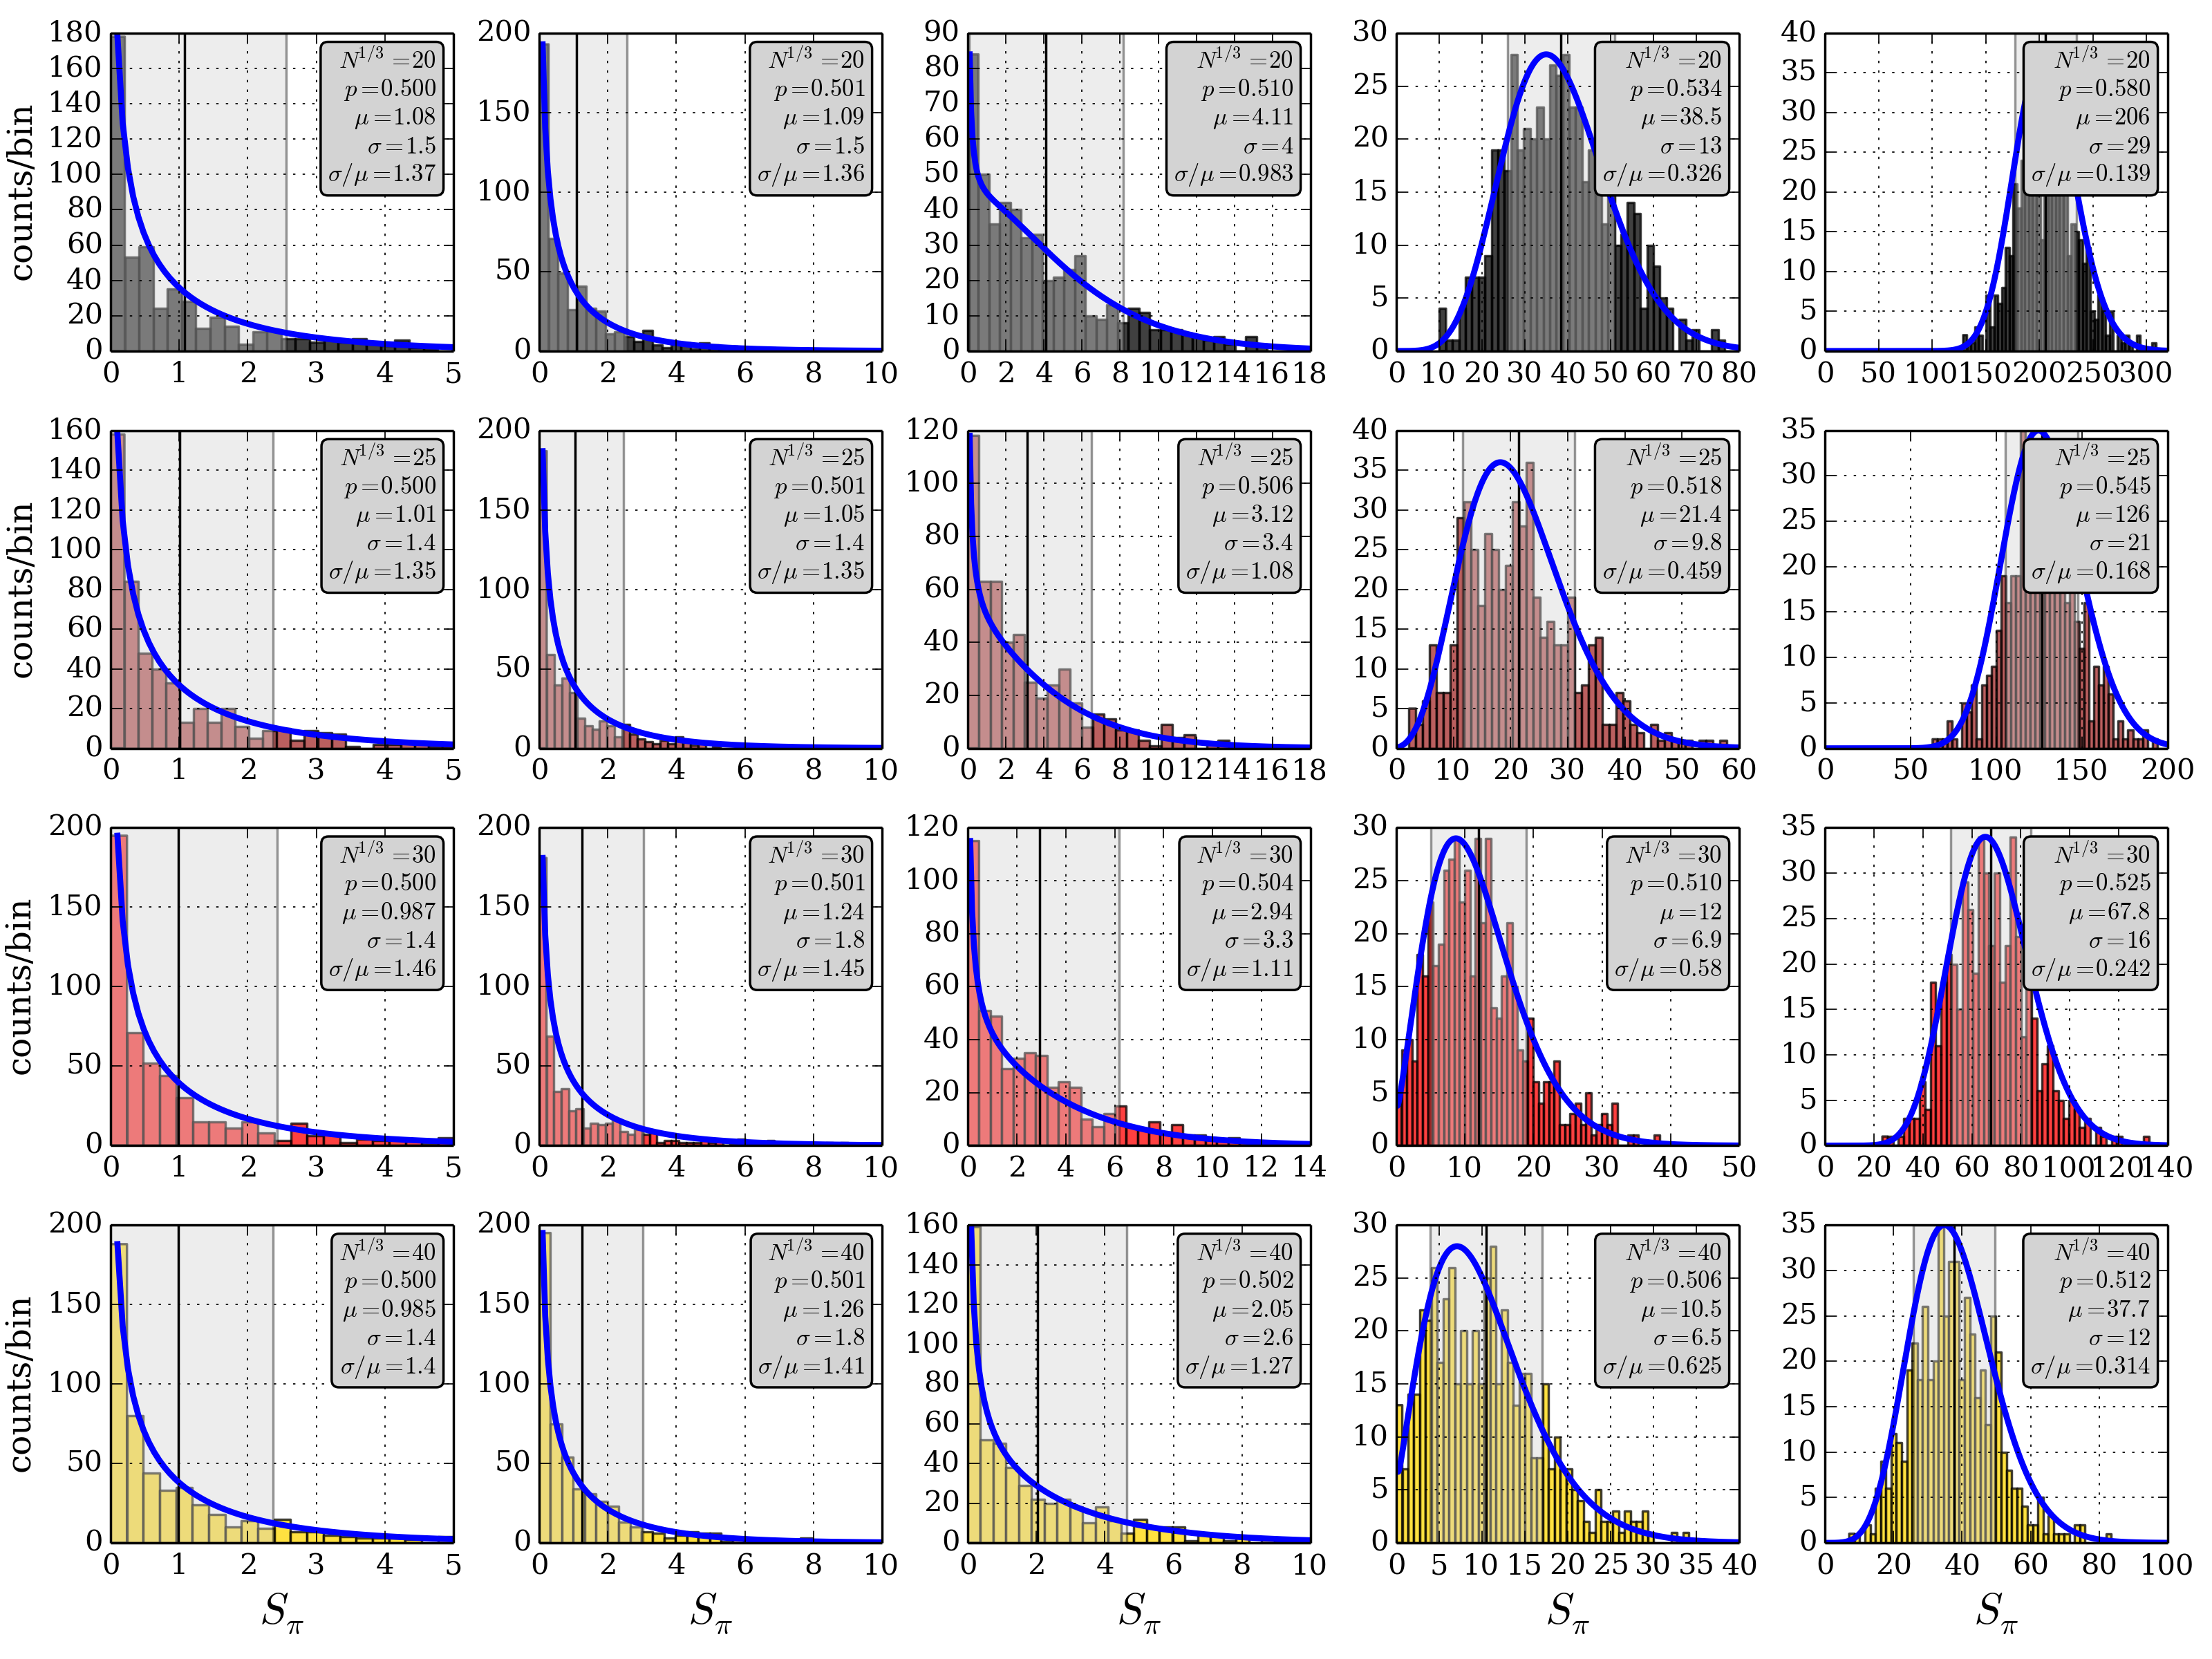
\includegraphics[width=\textwidth]{figures_140308/Noise_hist_p.png}
\caption[Fluctuations in $S_{\bv{\pi}}$]{\small Distribution of $S_{\bv{\pi}}$
for randomly ordered spins.  The spin ordering is parameterized by the
parameter $p$ as described in the text.  The probability density function
$P(S_{\bv{\pi}})$ as derived in the text is shown by the blue line.  The thin
black line denotes the mean of the distribution and the shaded gray area
denotes $\pm1$ standard deviations. }
\label{fig:spi-noise}
\end{figure}


\subsubsection{Results for an AFM ordered core} 

We can also consider a sample which has an AFM ordered domain of size
$L_{\text{AFM}}$ at the center and then a randomly ordered shell on the
outside.  Care is taken to make sure the spin mixture is balanced.  Numerically
realizing random distributions of the spins in the shell we can obtain the
distributions of $S_{\bv{\pi}}$ as a function of system size and size of the
AFM domain.  The results are shown in Fig.~\ref{fig:crystal-size}. 
\begin{figure}
\centering 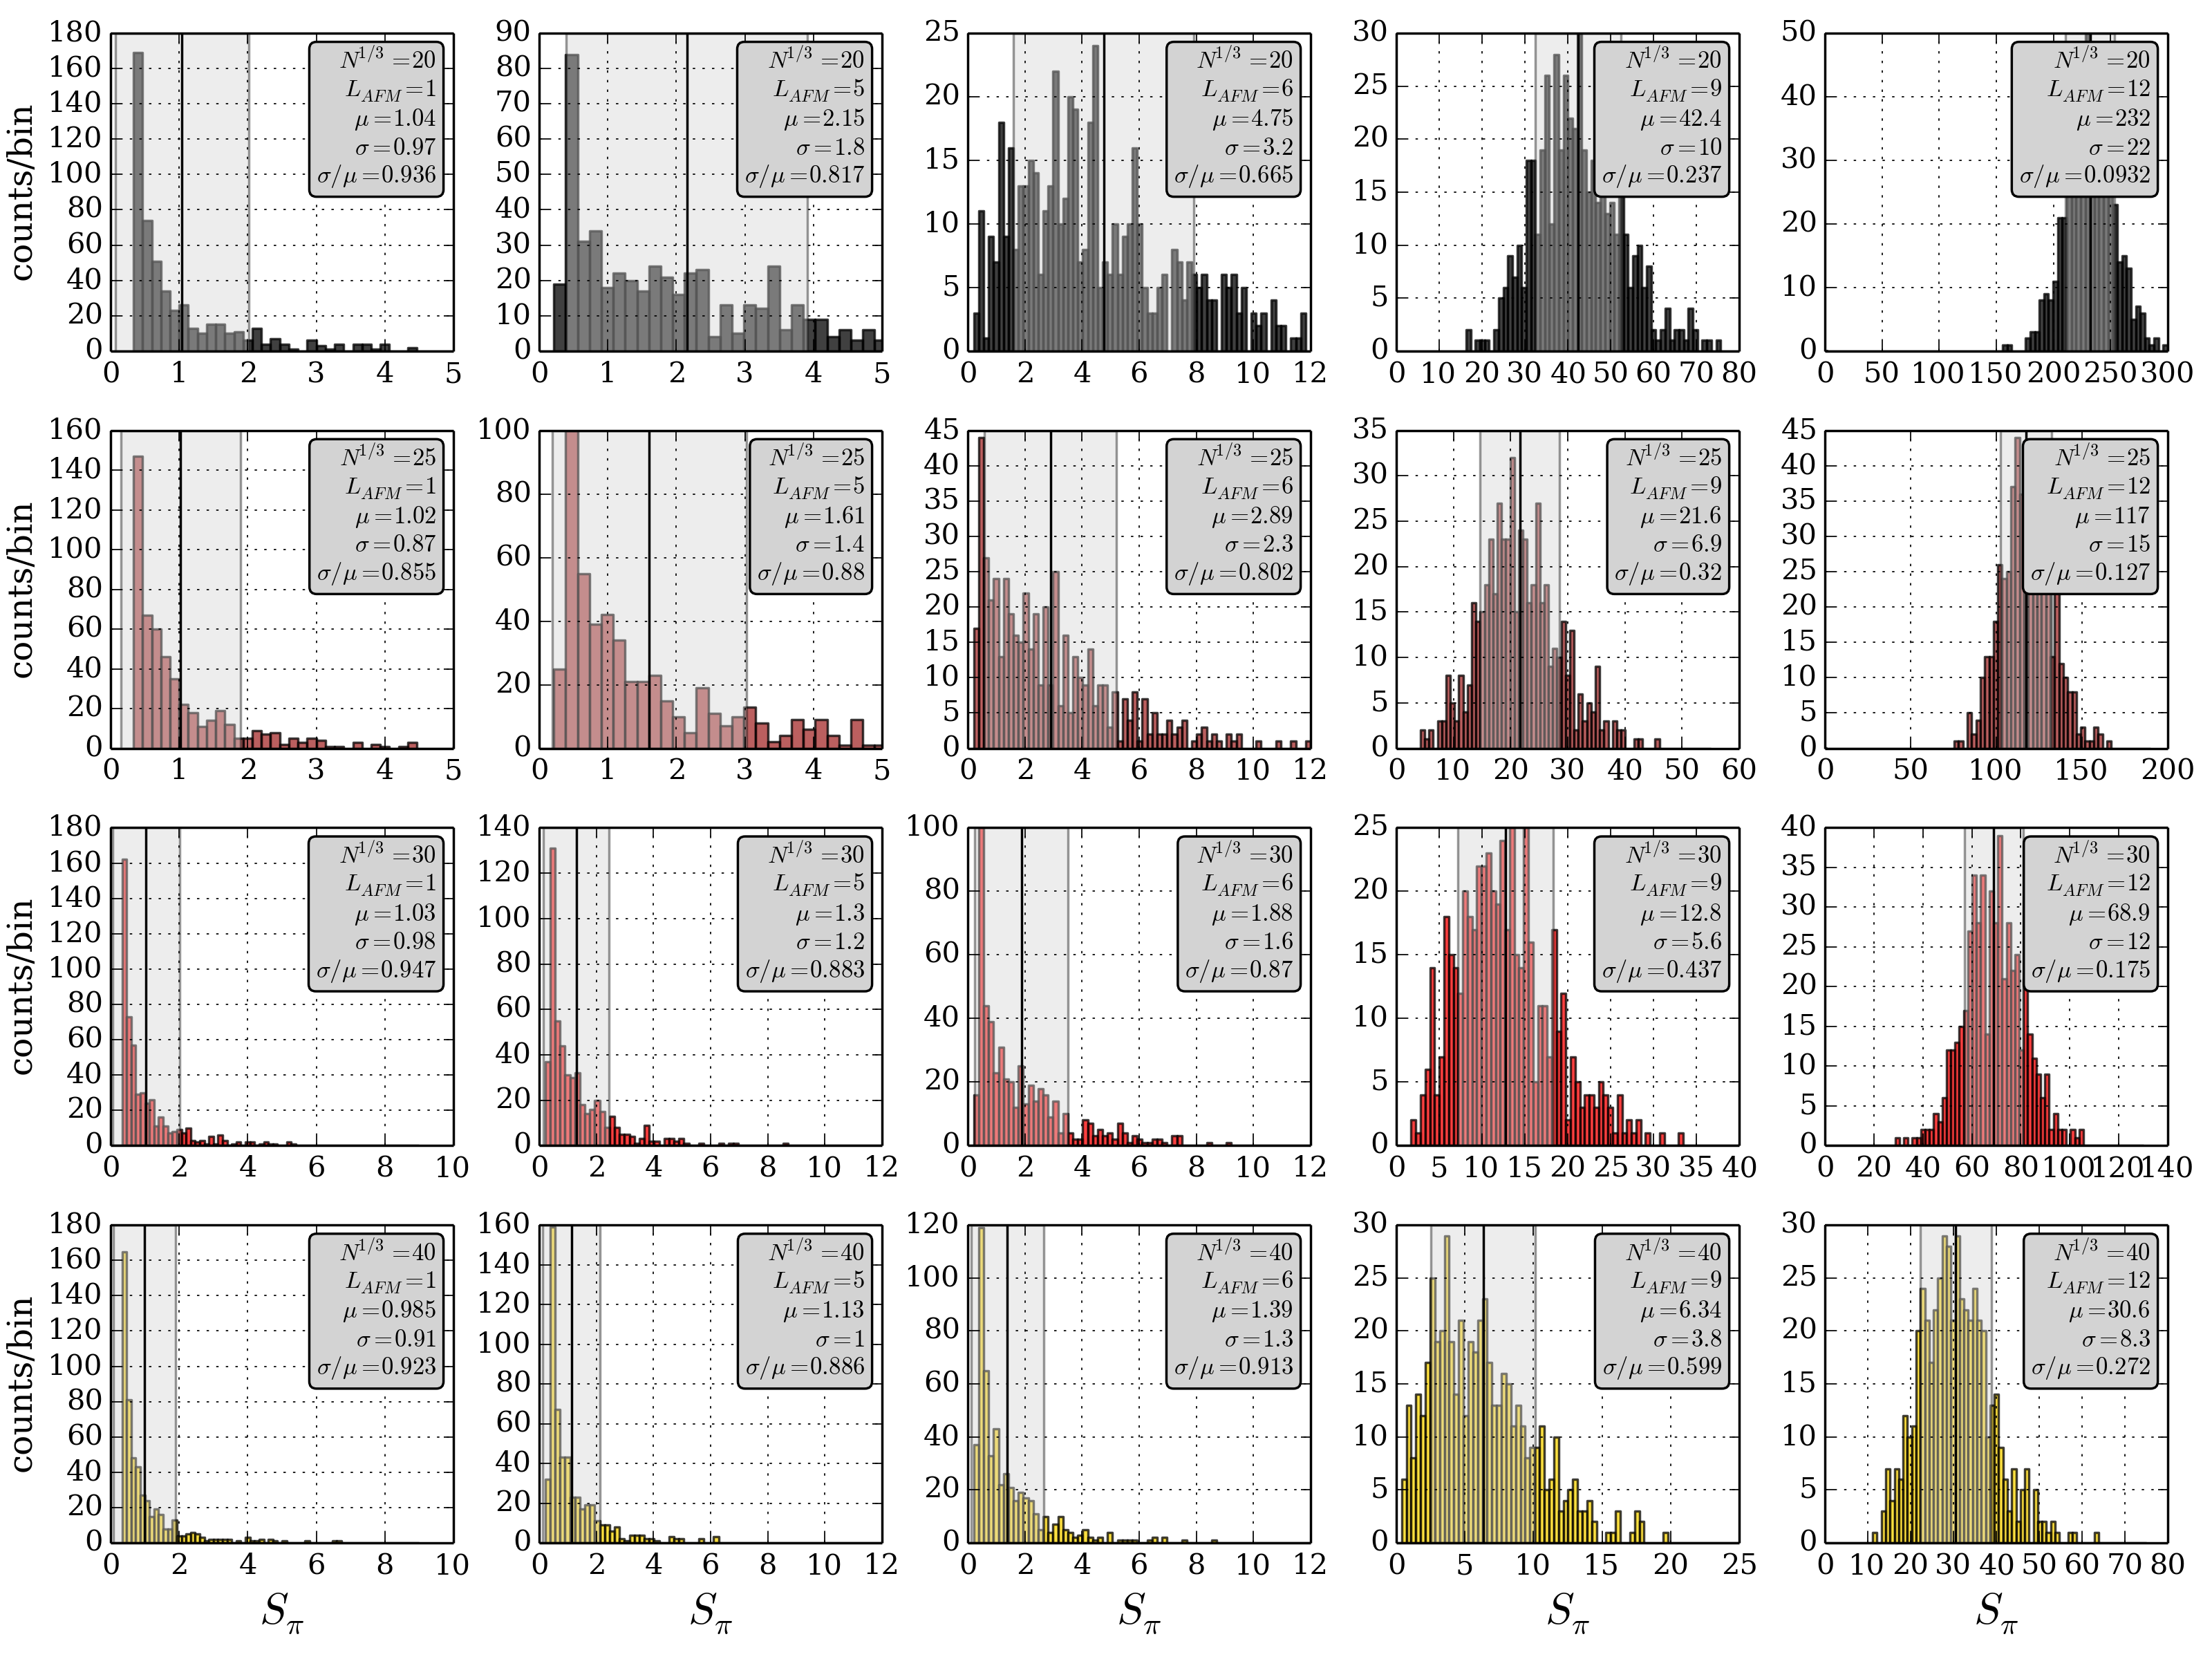
\includegraphics[width=\textwidth]{figures_140308/Noise_hist.png}
\caption[Fluctuations in $S_{\bv{\pi}}$]{\small Distribution of $S_{\bv{\pi}}$
for randomly ordered spins.  The spin ordering is parameterized by the size of
the AFM domain as described in the text.  The thin black line denotes the mean
and the shaded gray area denotes $\pm1$ standard deviations.  }
\label{fig:crystal-size}
\end{figure}

The mean values of the expected results at our detection cameras are shown for
various values of $N$ and $L_{\text{AFM}}$ in Fig.~\ref{fig:crystal-size-mean}. 
\begin{figure}
\centering 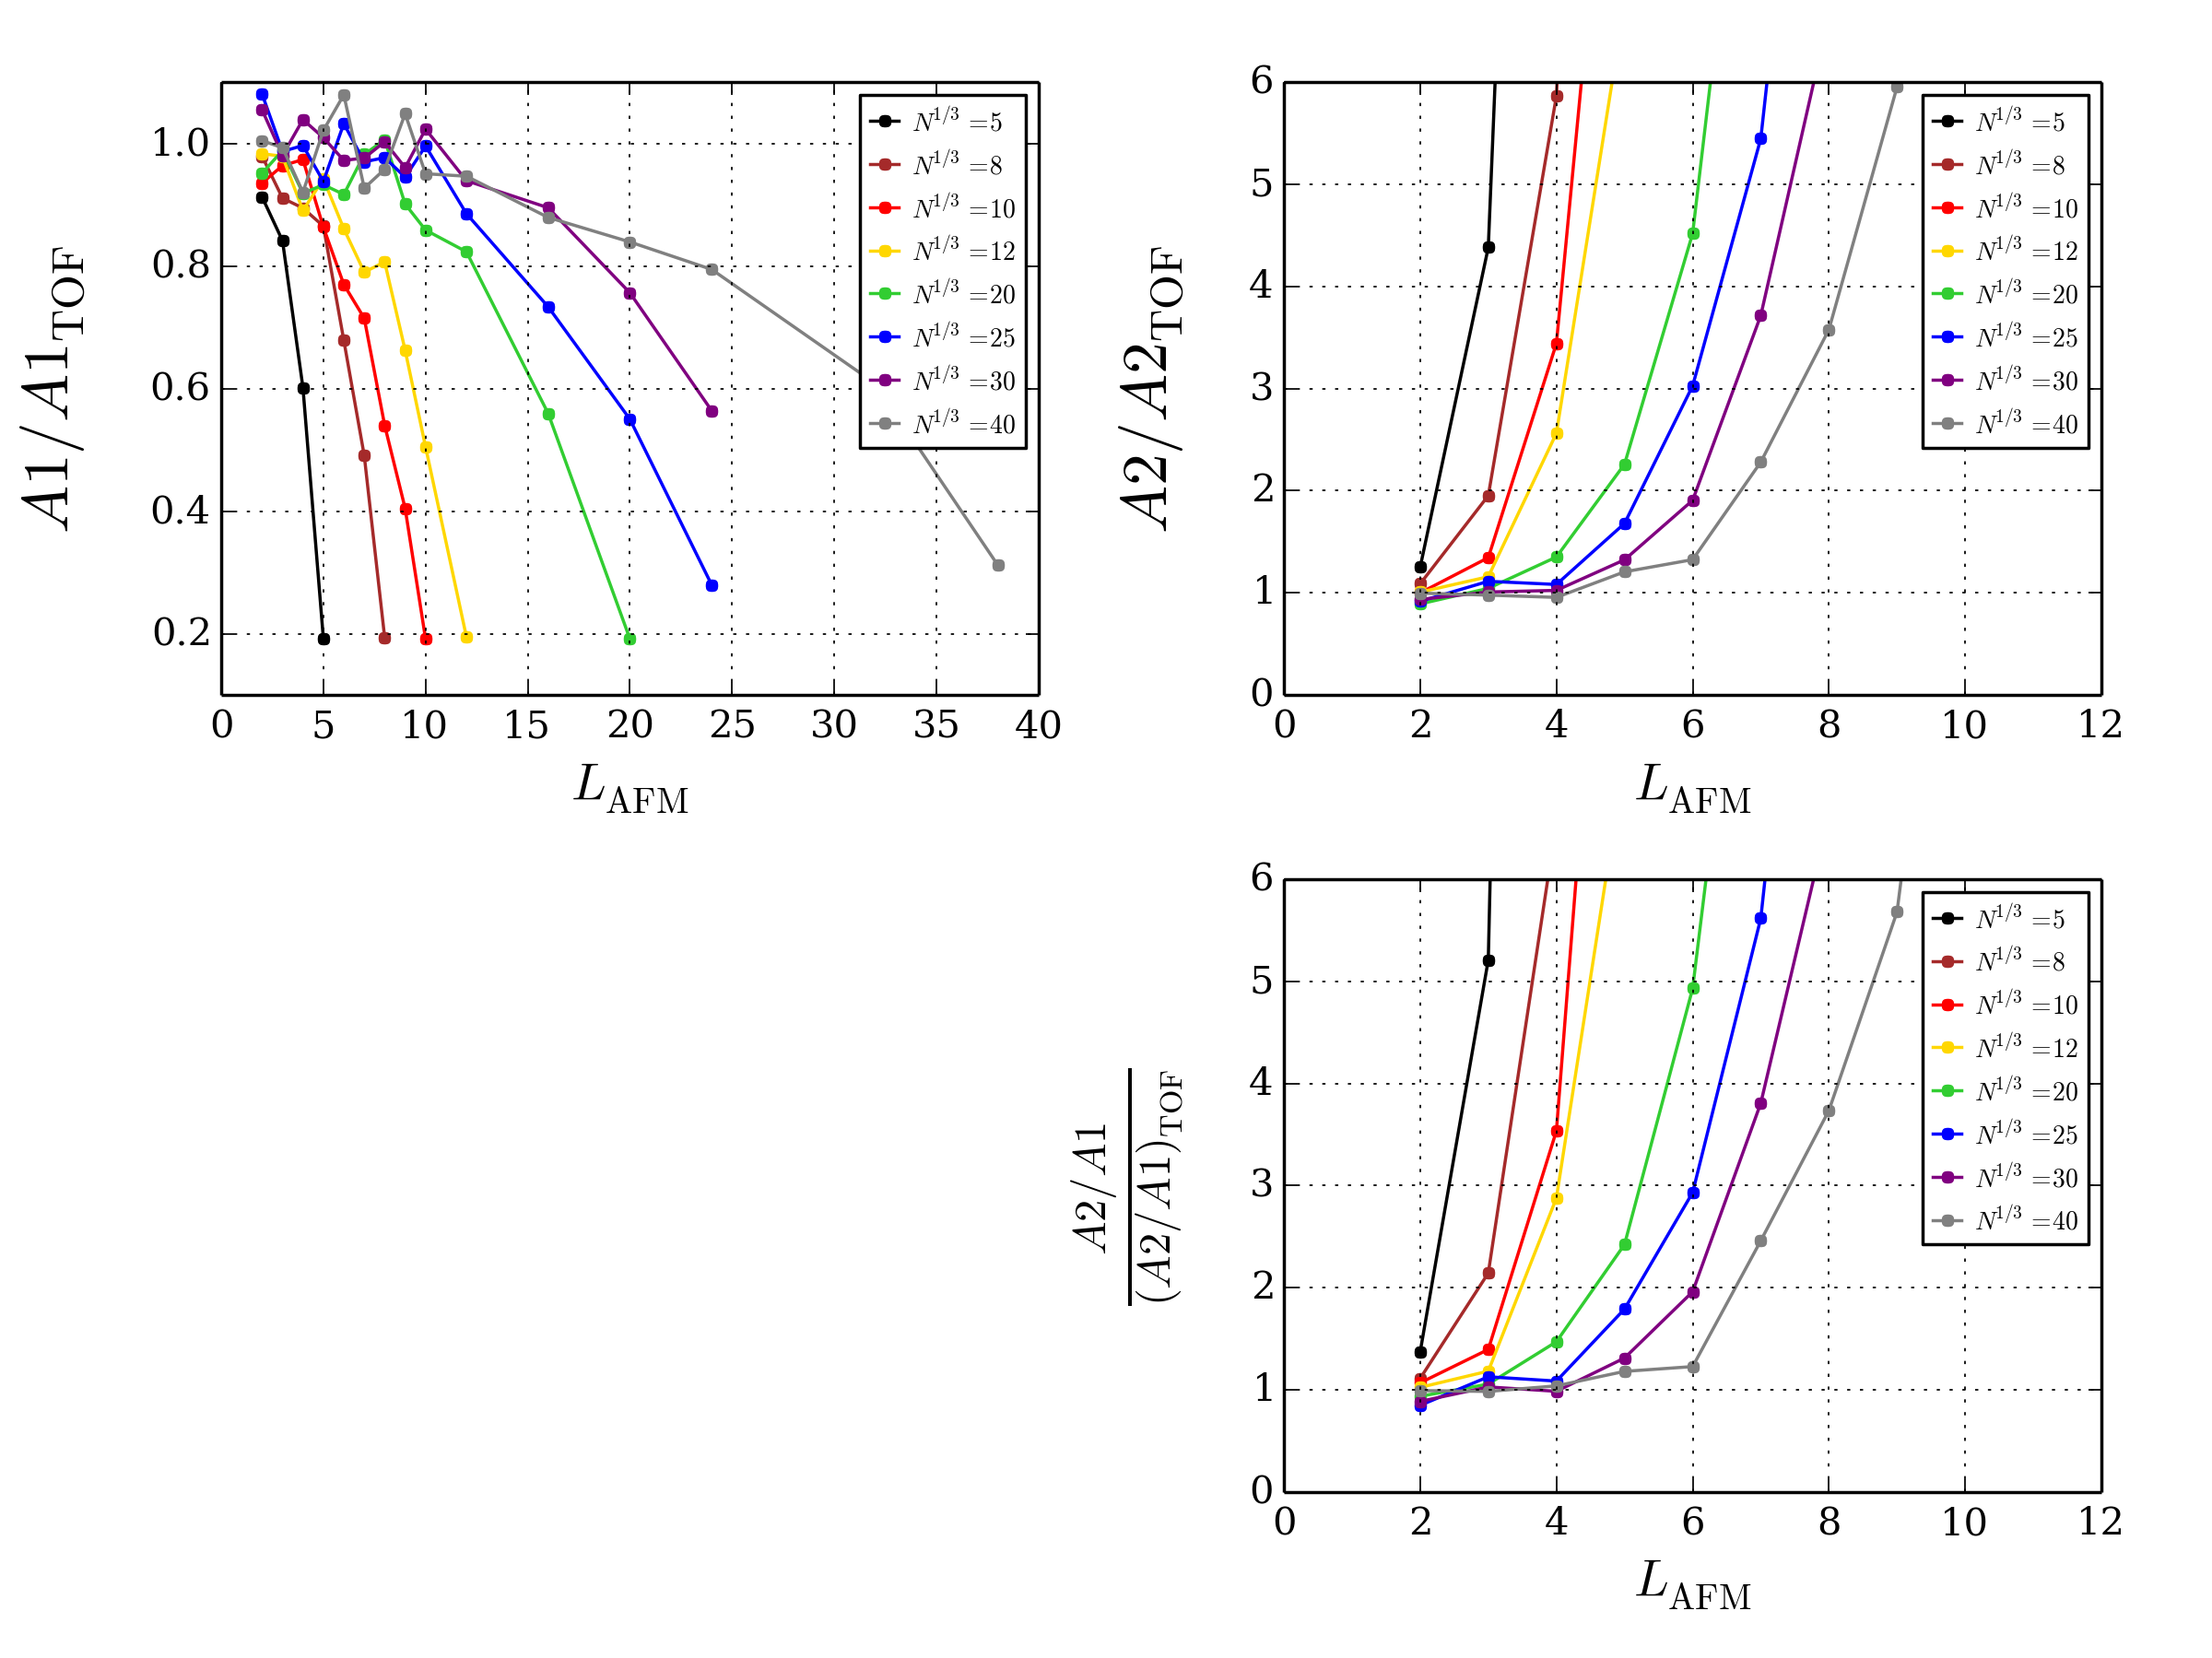
\includegraphics[width=\textwidth]{figures_140308/CrystalSize_plot.png}
\caption[Mean value of $S_{\bv{\pi}}$]{\small Mean value of $S_{\bv{\pi}}$
for randomly ordered spins.  The spin ordering is parameterized by the size of
the AFM domain as described in the text. }
\label{fig:crystal-size-mean}
\end{figure}

By plotting the mean, standard deviation and their ratio for the quantity
$S_{\bv{\pi}}$ we can see that the relative fluctuations only go down for
values of $S_{\bv{\pi}}$ significantly larger than 1,  which is a regime that
would only be attained below the Neel transition.   This is shown in
Fig.~\ref{fig:spi-variance}.
\begin{figure}
\centering 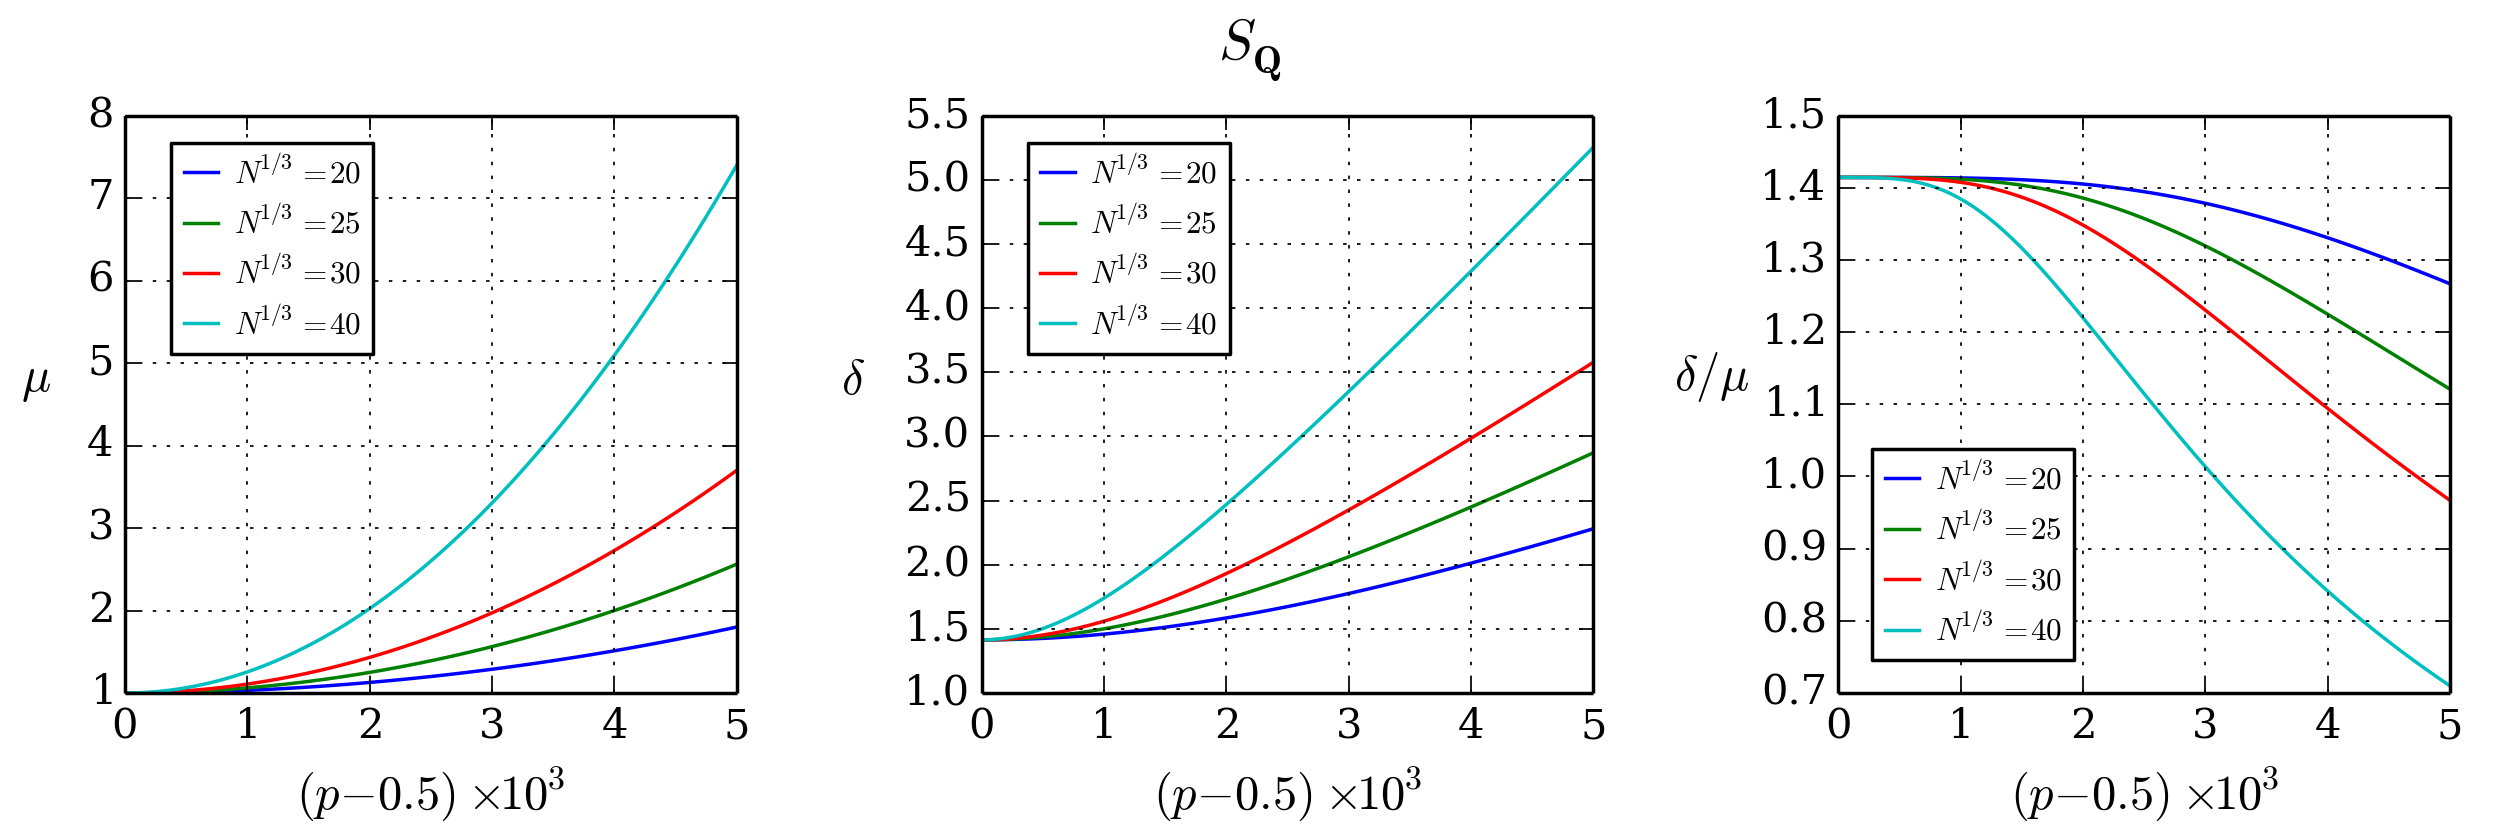
\includegraphics[width=\textwidth]{figures_140308/spi-variance.png}
\caption[Mean value and variance of $S_{\bv{\pi}}$]{\small Mean value,
variance, and their ratio for $S_{\bv{\pi}}$ are plotted for different values
of $p$, and $N$.  }
\label{fig:spi-variance}
\end{figure}


\newpage


\subsection{Angular dependence of $S_{\bv{Q}}$ }

In this section we wish to obtain the analytical dependence of the spin
structure factor $S_{\bv{Q}}$ as a function of $\bv{Q}$.   We assume that the
spin-spin correlation function has a correlation length $L_{c}$,  so we can
write
\begin{equation}
 \langle S_{zm}S_{zn} \rangle  =   
   \frac{1}{4} 
   e^{-i\bv{\pi}( \bv{R}_{m} - \bv{R}_{n}) } 
   e^{-|\bv{R}_{m} - \bv{R}_{n}| / L_{c} } 
\end{equation} 
Here $\bv{\pi} = \frac{2\pi}{a}(1/2,\,1/2,\,1/2)$ ensures that the spins are
antiferromagnetically ordered and their correlation decays over a length
$L_{c}$.  

Our goal is to obtain the spin structure factor, which is defined as  
\begin{equation}
\begin{split}
S_{\bv{Q}} & =  
      \frac{4}{N}
      \sum_{mn}  
      e^{ i \bv{Q}( \bv{R}_{m} - \bv{R}_{n} ) }  
      \langle S_{zm}S_{zn} \rangle 
  = 
      \frac{4}{N}
      \sum_{mn}  
      e^{ i \bv{Q}( \bv{R}_{m} - \bv{R}_{n} ) }  
   \frac{1}{4} 
   e^{-i\bv{\pi}( \bv{R}_{m} - \bv{R}_{n}) } 
   e^{-|\bv{R}_{m} - \bv{R}_{n}| / L_{c} } \\ 
   & = 
   \frac{1}{N} 
      \sum_{mn}  
      e^{ i (\bv{Q}-\bv{\pi})( \bv{R}_{m} - \bv{R}_{n} ) }  
   e^{-|\bv{R}_{m} - \bv{R}_{n}| / L_{c} }
\end{split} 
\end{equation}
We introduce the vector $\bv{p}=\bv{Q}-\bv{\pi}$ and split the sum into $m=n$
and $m\neq n$ parts:
\begin{equation}
\begin{split} 
S_{\bv{Q}}  & = 
   \frac{1}{N}\left(  
   \sum_{m=n} + 
      \sum_{m\neq n} \right) 
      e^{ i \bv{p}( \bv{R}_{m} - \bv{R}_{n} ) }  
   e^{-|\bv{R}_{m} - \bv{R}_{n}| / L_{c} }  \\
   & =  
   1 +  \sum_{m\neq n }  
      e^{ i \bv{p}( \bv{R}_{m} - \bv{R}_{n} ) }  
   e^{-|\bv{R}_{m} - \bv{R}_{n}| / L_{c} }  \\
\end{split}
\end{equation}

We change one of the indices in the sum according to
$\bv{R}_{m} = \bv{R}_{n} + \bv{R}_{k}$, which gives
\begin{equation}
S_{\bv{Q}} = 1+  
   \frac{1}{N} 
      \sum_{n}\sum_{k\neq 0}  
      e^{ i \bv{p}\bv{R}_{k} } 
   e^{-|\bv{R}_{k}| / L_{c} }  
   = 1+ 
      \sum_{k\neq 0}  
      e^{ i \bv{p}\bv{R}_{k} } 
   e^{-|\bv{R}_{k}| / L_{c} }  
\end{equation}
Notice that on the second step above we have carried out the sum over $n$,
assuming that the crystal is sufficiently large such that there are no edge
effects associated with the translation that was performed upon changing the
index variables.  This is a valid assumption as long as the correlation length,
$L_{c}$ is significantly smaller than the size of the entire crystal. 

We will now approximate the sum over $k$ with an integral, $\sum_{k\neq 0}
\rightarrow a^{-3}\int_{\mathbb{R}^{3}} \mathrm{d}^{3}\mathbb{R}$,  where $a$
is the lattice spacing. 
\begin{equation}
S_{\bv{Q}} = 1 +  
      \sum_{k\neq 0 }  
      e^{ i \bv{p}\bv{R}_{k}  }  
   e^{-|\bv{R}_{k}| / L_{c} }  
     =  1 + 
   \frac{1}{a^{3}} 
   \int_{\mathbb{R}^{3}} \mathrm{d}^{3}\mathbb{R}  \, 
      e^{ i \bv{p}\bv{R}_{k}  }  
   e^{-|\bv{R}_{k}| / L_{c} }  
\end{equation}
The integral that remains is the 3D Fourier transform of a spherically
symmetric function.   We will show below that this can be replaced by the
Fourier-Bessel transform of the radial function  $e^{-R/L_{c}}$.   

Let's look at the Fourier transform $F(\bv{p})$ of a spherically symmetric
function $f(R)$, choosing the polar axis to be along $\bv{p}$:
\begin{equation}
 F(\bv{p}) = 
   \int_{\mathbb{R}^{3}} \mathrm{d}^{3}\mathbb{R} \, 
    e^{i \bv{p}\bv{R}} f(R)  
    = 
   \int_{0}^{\infty} \int_{0}^{\pi} \int_{0}^{2\pi} 
    e^{i p R \cos\theta} f(R) R^{2}\, \mathrm{d}R \,\sin\theta \mathrm{d}\theta\,
    \mathrm{d}\phi 
\end{equation}
We will replace $\theta$ according to $x=\cos\theta$, $\mathrm{d}x =
\sin\theta\mathrm{d}\theta$. 
\begin{equation}
\begin{split}
 F(\bv{p})  & = 
   2 \pi \int_{0}^{\infty} f(R) R^{2} 
   \left[ \int_{-1}^{1} e^{ i pRx} \,\mathrm{d}x \right] \mathrm{d}R
   =  
   2 \pi \int_{0}^{\infty} f(R) R^{2} 
   \left[ \frac{ e^{ipR} - e^{-ipR}}{ipR} \right] \mathrm{d}R \\
   & =  
   4 \pi \int_{0}^{\infty} f(R)
   \frac{ \sin(pR)}{pR}\, R^{2} 
  \mathrm{d}R
\end{split}
\end{equation}
This last expression is the Fourier-Bessel transform of $f(R)$.   

Applying this result to the integral in the definition of the structure factor,
we have
\begin{equation}
S_{\bv{Q}} = 1 +  
   \frac{4\pi}{a^{3}}
   \int_{0}^{\infty}  
   e^{-R/ L_{c} }  
   \frac{ \sin(pR)}{pR}\, R^{2} 
  \mathrm{d}R
\end{equation}

This last integral can be plugged into Mathematica to obtain
\begin{equation}
S_{\bv{Q}} - 1 = 
    \frac{8\pi}{a^{3}} 	\frac{ L_{c}^{3} }
     { \left[ 1 + (L_{c} |\bv{Q}-\bv{\pi}|)^{2}  \right]^{2} } 
\end{equation}

We want to obtain the angular dependence of $S_{\bv{Q}}$ when changing the
input angle of the probe light used for Bragg scattering.  Suppose the vectors
$\bv{k}_{\text{in}0}$ and $\bv{k}_{\text{out}0}$ satisfy the Bragg condition,
such that
\begin{equation}
 \bv{k}_{\text{in}0} - 
 \bv{k}_{\text{out}0}   = \bv{\pi} 
\end{equation} 
If we rotate the input direction slightly by an angle $\alpha$, then 
\begin{equation} 
 \bv{k}_{\text{in}} = 
 \bv{k}_{\text{in}0}  +  
 |\bv{k}_{\text{in}0}|\alpha \bv{\hat{n}}_{0}
\end{equation}
where $\bv{\hat{n}}_{0}$ is a unit vector perpendicular to
$\bv{k}_{\text{in}0}$.  We then have that 
\begin{equation} 
 p = | \bv{Q} - \bv{\pi} | = 
 | \bv{k}_{\text{in}} - 
 \bv{k}_{\text{out}0}  - \bv{\pi}  | =
 |\bv{k}_{\text{in}0}  +  
 |\bv{k}_{\text{in}0}|\alpha \bv{\hat{n}}_{0} - 
 \bv{k}_{\text{out}0}  - \bv{\pi} |  = 
 |\bv{k}_{\text{in}0}|\alpha  = \frac{2\pi}{\lambda_{B}} \alpha  
\end{equation}
where $\lambda_{B}$ is the wavelength of the Bragg probe.

We then have that for a small angular change $\alpha$ in the input Bragg probe
\begin{equation}
S(\alpha) - 1 = 
    8\pi \frac{ (L_{c}/a)^{3} }
     { \left[ 1 + \left(\frac{2\pi L_{c}}{\lambda_{B}} \alpha \right)^{2}   \right]^{2} } 
\end{equation}
or 
\begin{equation}
\frac{S(\alpha) - 1}{ S_{\bv{\pi}}} = 
     \frac{ 1 }
   { \left[ 1 + \left(\frac{2\pi L_{c}}{\lambda_{B}} \alpha \right)^{2}  
        \right]^{2} } 
  \approx \exp\left[ -2 \left( \frac{2\pi}{\lambda_{B}} L_{c} \alpha\right)^{2} \right]
\end{equation}
We see  that the $1/e$ radius of the angular profile is given by
\begin{equation}
 \alpha_{1/e} = \frac{ \lambda_{B}}{ 2\pi\sqrt{2}} \frac{1}{L_{c}}  
  =  \frac{ \lambda_{B}/a}{ 2\pi\sqrt{2}} \frac{1}{L_{c}/a}  
  =   \frac{0.14}{L_{c}/a} 
\end{equation}

Alternately we can consider a spin-spin correlation function that is shaped
like a box of length $L_{\text{AFM}}$: 
\begin{equation}
 \langle S_{zm}S_{zn} \rangle  =  
  \begin{cases}  
   \frac{1}{4} &   \text{if}\ |\bv{R}_{m}-\bv{R}_{n}| \leq L_{\text{AFM}}\\ 
   0           &   \text{if}\ |\bv{R}_{m}-\bv{R}_{n}| > L_{\text{AFM}}\\ 
  \end{cases}
\end{equation}

In this case we find that 
\begin{equation}
\begin{split}
S_{\bv{Q}} & = 1 +  
   \frac{4\pi}{a^{3}}
   \int_{0}^{ L_{\text{AFM}}}  
   \frac{ \sin(pR)}{pR}\, R^{2} 
  \mathrm{d}R \\
   & = 1 + 
   \frac{4\pi}{a^{3}} \left[
   \frac{ \sin\left( p L_{\text{AFM}}\right ) 
              - p L_{\text{AFM}} \cos\left( p L_{\text{AFM}} \right) }
   { p^{3}} \right]
\end{split}
\end{equation}

\begin{equation}
\begin{split}
  \frac{ S(\alpha) - 1 }{ S_{\bv{\pi}} } & = 
   \frac{3}{L_{\text{AFM}}^{3}} 
   \frac{ \sin\left( \frac{2\pi L_{\text{AFM}}}{\lambda_{B}}\alpha\right ) 
              - \frac{2\pi\alpha}{\lambda_{B}} L_{\text{AFM}} 
     \cos\left( \frac{ 2\pi L_{\text{AFM}} }{\lambda_{B}} \alpha\right) }
   { p^{3}} \\ 
   & 
  \approx \exp\left[ - \frac{1}{10} \left( \frac{2\pi}{\lambda_{B}} L_{c} \alpha\right)^{2} \right]
\end{split}
\end{equation}

In this case the $1/e$ radius of the angular profile is given by 
\begin{equation}
 \alpha_{1/e} = \frac{ \lambda_{B}}{ 2\pi} \sqrt{10} \frac{1}{L_{c}}  
  =  \frac{ \lambda_{B}/a}{ 2\pi} \sqrt{10} \frac{1}{L_{c}/a}  
  =   \frac{0.634}{L_{c}/a} 
\end{equation}


The $1/e$ radii obtained for an exponentially decaying correlation and for a
correlation function that looks like a box differ by a factor of 634/140= 4.52
which is somewhat unexpected. A comparison of
the two angular functions is shown in Fig.~\ref{fig:salpha-fourier}. 
\begin{figure}
\centering
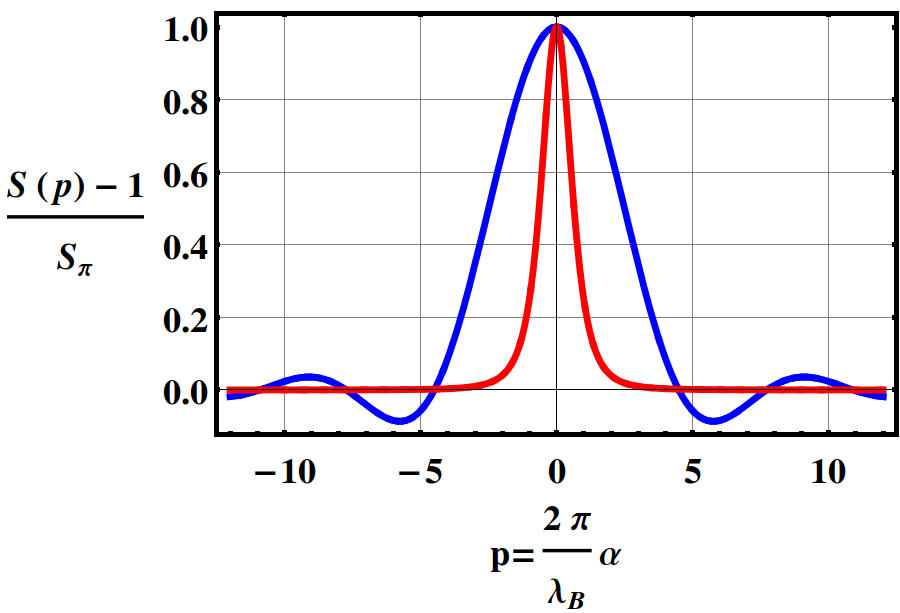
\includegraphics[width=0.6\textwidth]{figures_140308/rocking-fourier.png}
\caption[Angular variation of $S_{\bv{Q}}$]{\small Angular variation of
$S_{\bv{Q}}$ as a function of $p=\frac{2\pi\lambda_{B}}{\alpha}$  where
$\alpha$ is a small angular deviation of the input Bragg beam.  The blue line
is for the box correlation function and the red line is for the exponential
decay correlation function. }
\label{fig:salpha-fourier}
\end{figure}


 

\subsubsection{Angular dependence of $S_{\bv{Q}}$ for a matrix of randomly
ordered spins}

We have performed simulations of Bragg scattering on  a 3D lattice of randomly
ordered spins.  The lattice has an AFM ordered core with size $L_{\text{AFM}}$
at the center  and a randomly ordered shell on the outside.  The total number
of spins in the lattice is $N$, and the lattice is a cube with side equal to
$N^{1/3}$.

Below we will plot the results of varying the angle of incidence of the probe Bragg
beam, by a small amount around the value that satisfy the Bragg condition.   We
also show the results of varying the observation angle slightly away from the
angle that satisfies the Bragg condition.   These two variations are referred
to as input rocking curve and output rocking curve respectively. 

We show plots of the input and output rocking curve, and the $1/e$ radii of the
angular distributions as a function of the AFM core size.  We do this for
crystal sizes of $N^{1/3} = 20, 30, 40, 50$, as shown if
Figs.~\ref{fig:rocking20}-\ref{fig:rocking50}.   
\begin{figure}
\centering 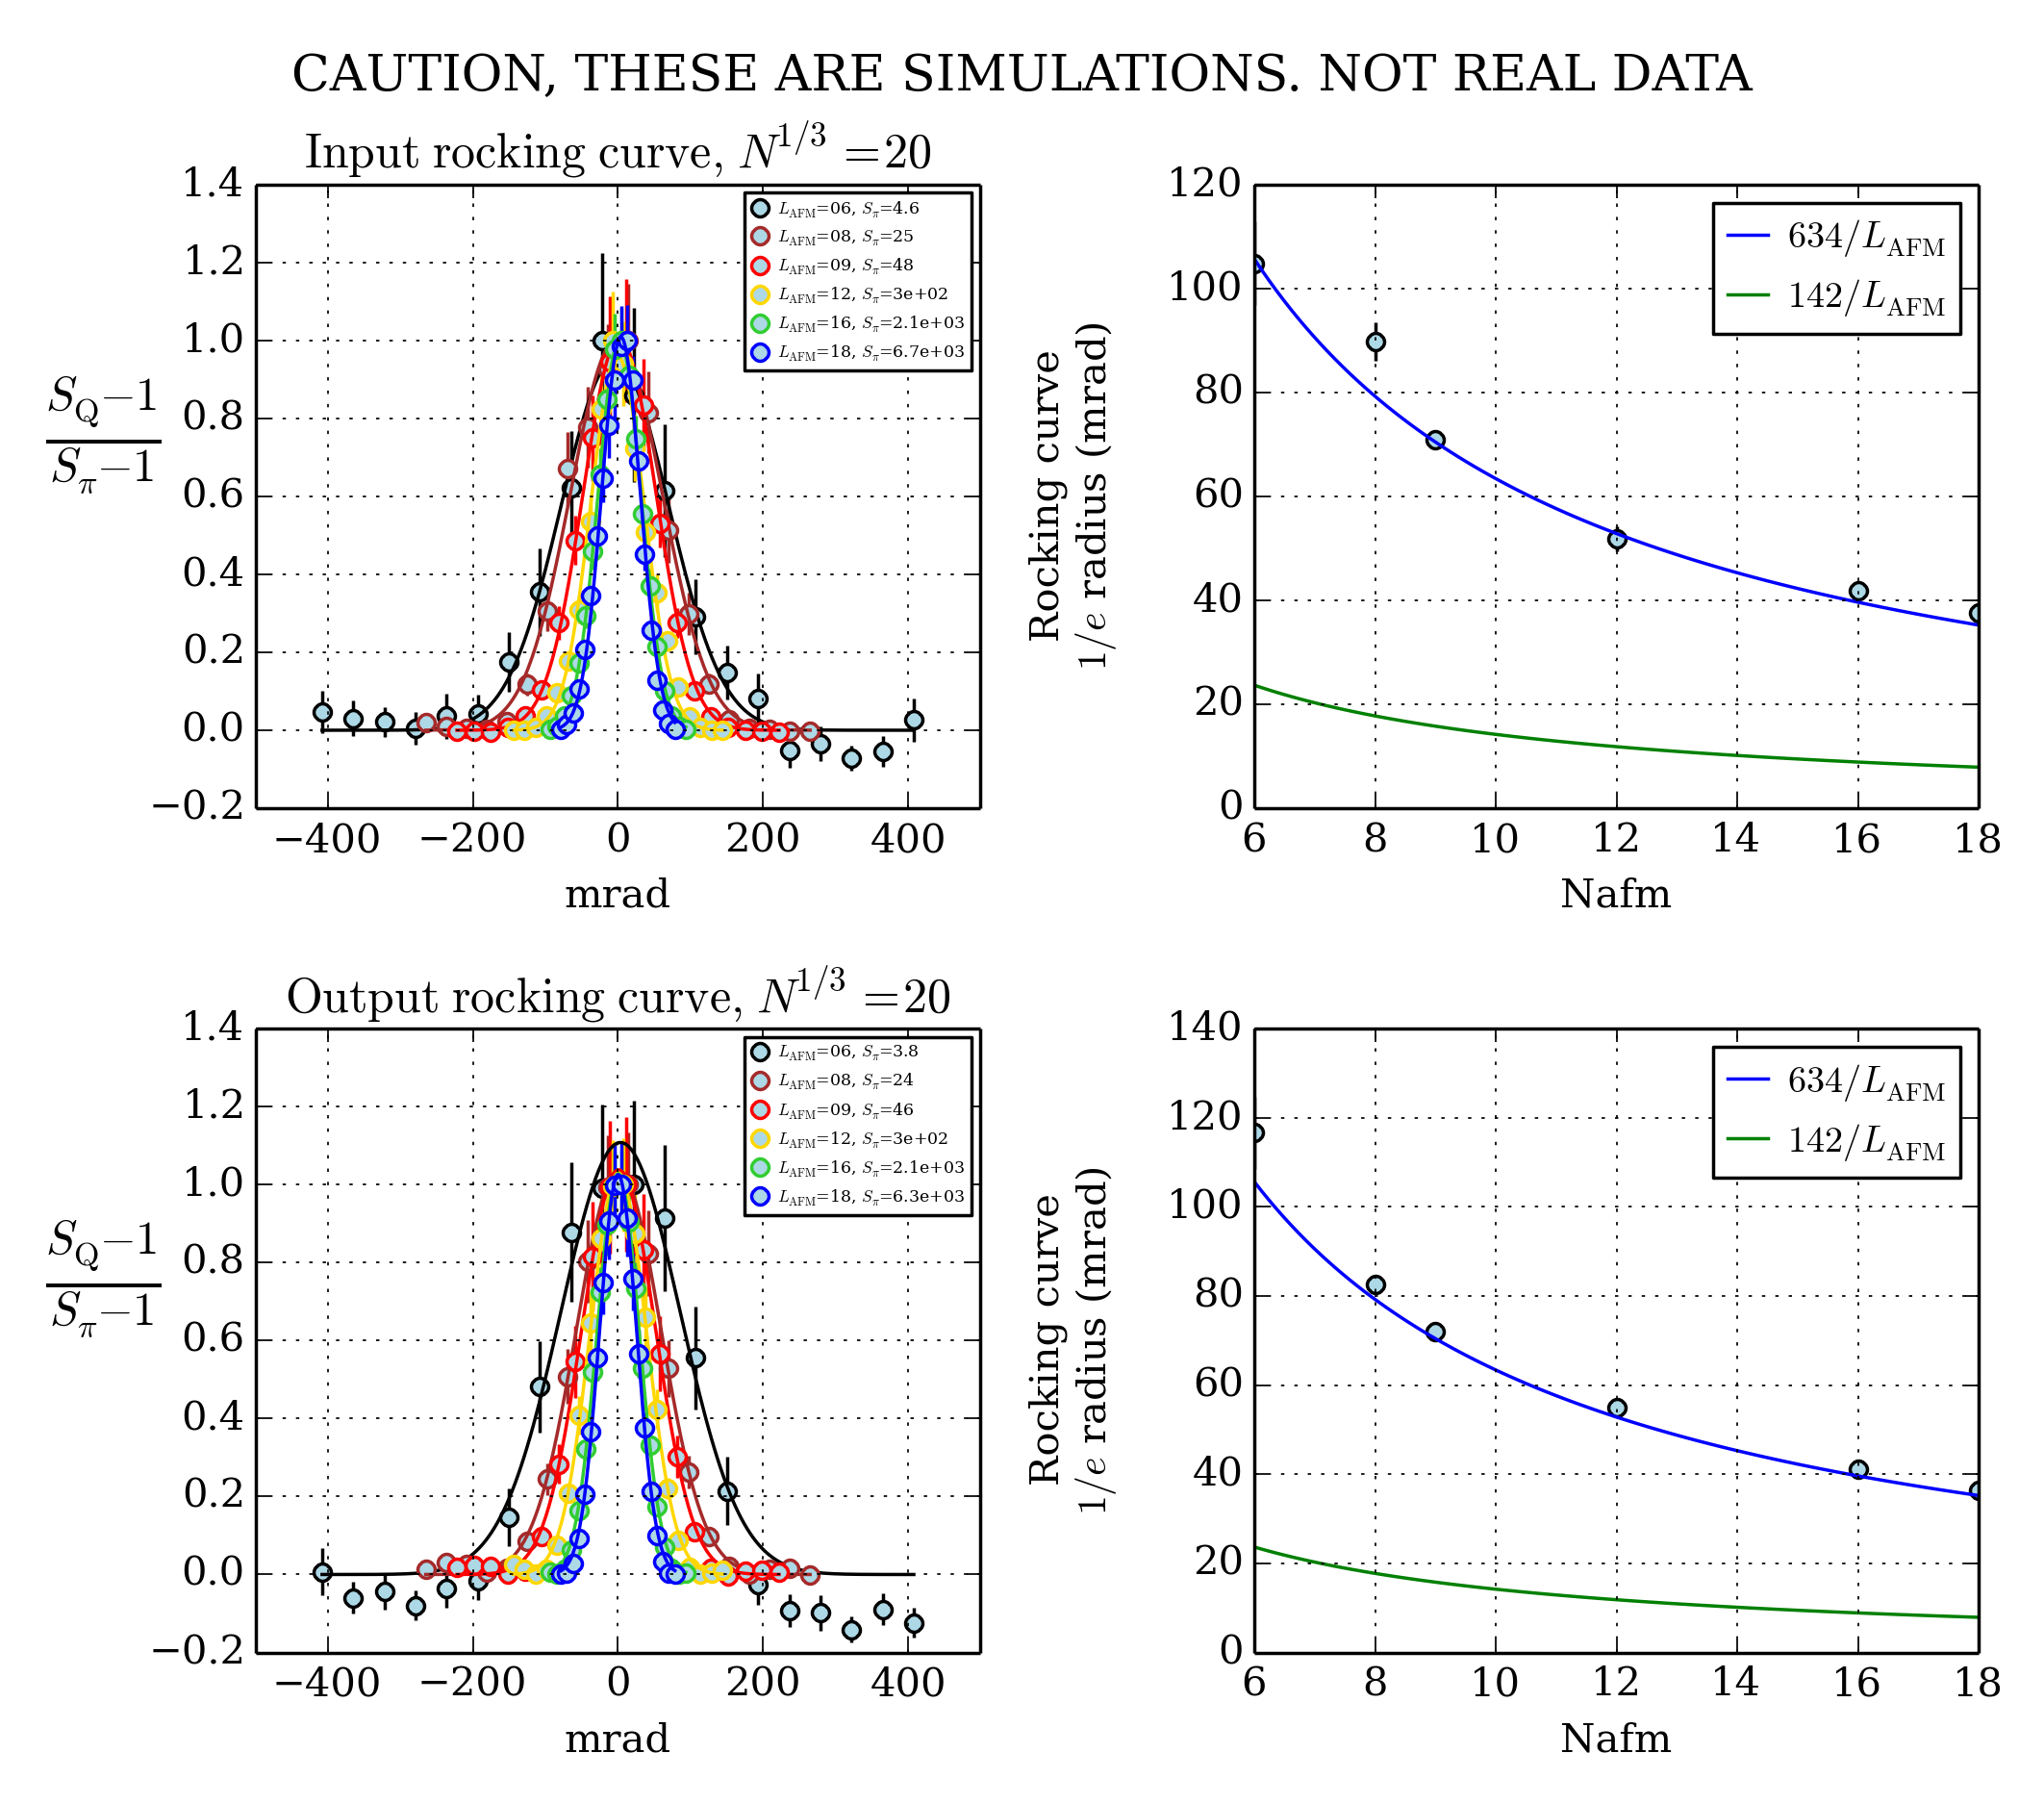
\includegraphics[width=0.6\textwidth]{figures_140308/Rocking_20.png}
\caption[Rocking curve for $N^{1/3}$=20]{\small Rocking curve for $N^{1/3}$=20.
The blue line is the analytical result for the box function correlations and
the green line is the analytical result for the exponentially decaying
correlations.  }
\label{fig:rocking20}
\end{figure}
\begin{figure}
\centering 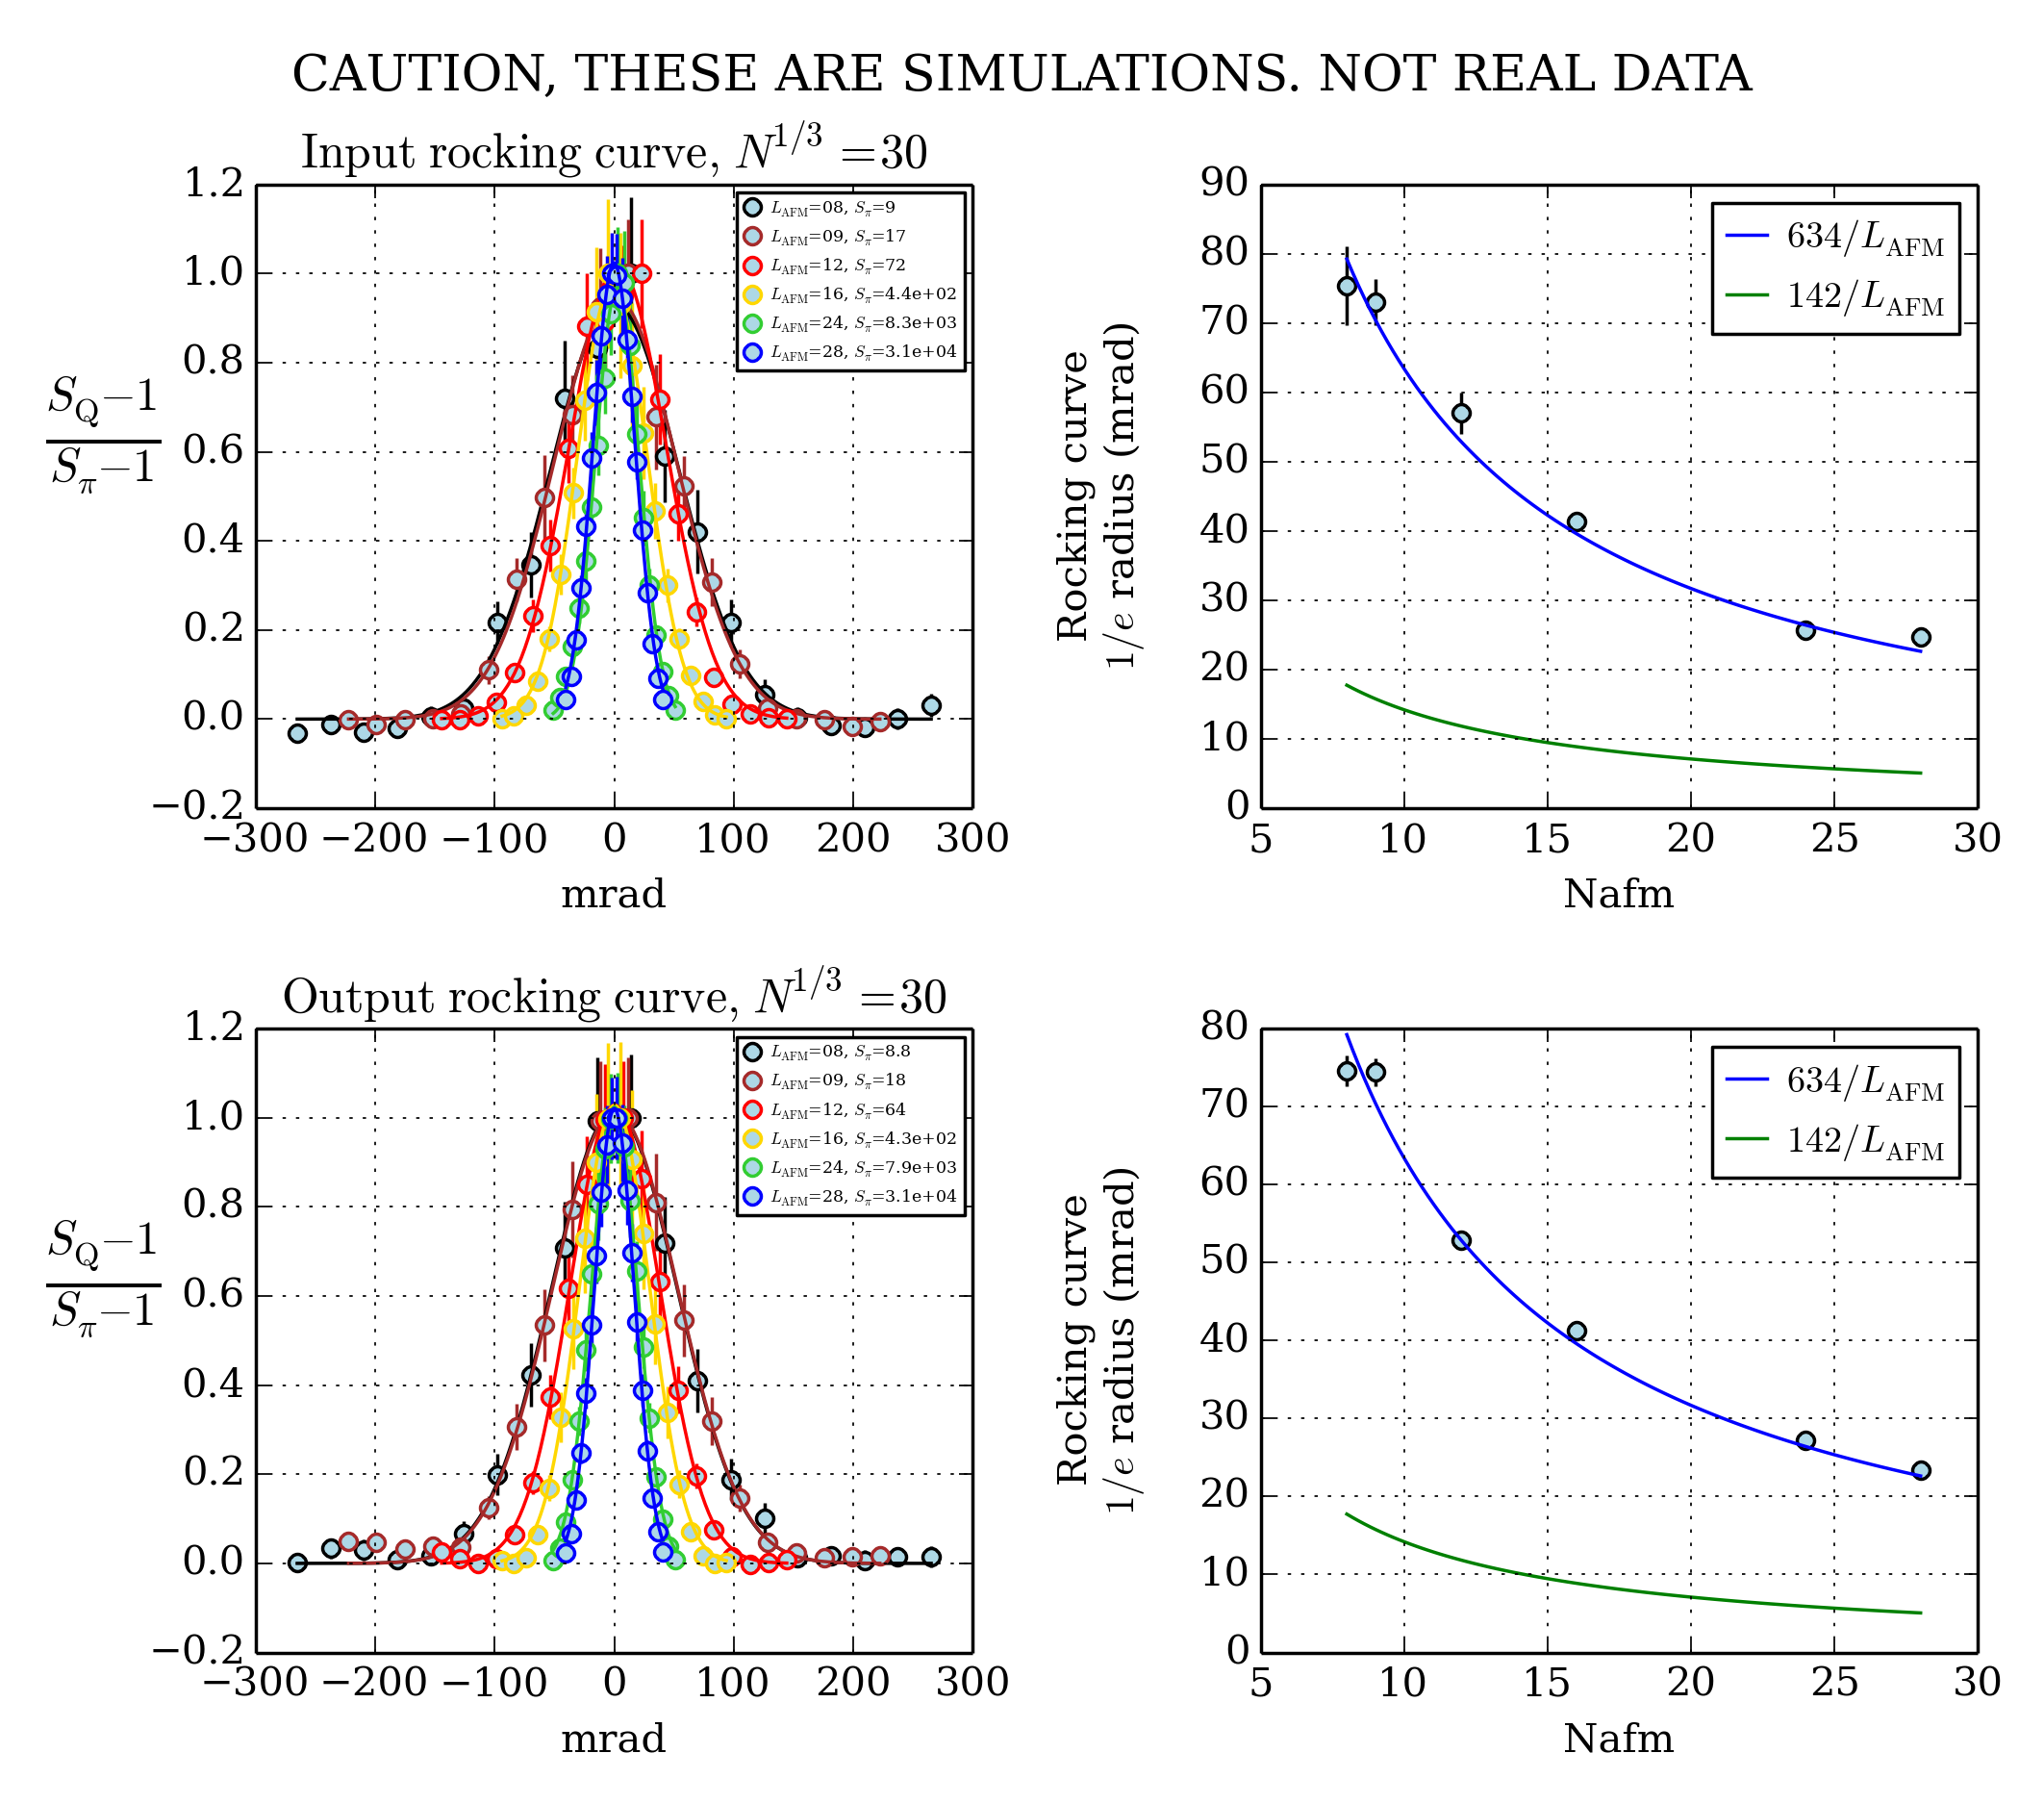
\includegraphics[width=0.6\textwidth]{figures_140308/Rocking_30.png}
\caption[Rocking curve for $N^{1/3}$=30]{\small Rocking curve for $N^{1/3}$=30.
The blue line is the analytical result for the box function correlations and
the green line is the analytical result for the exponentially decaying
correlations.  }
\label{fig:rocking30}
\end{figure}
\begin{figure}
\centering 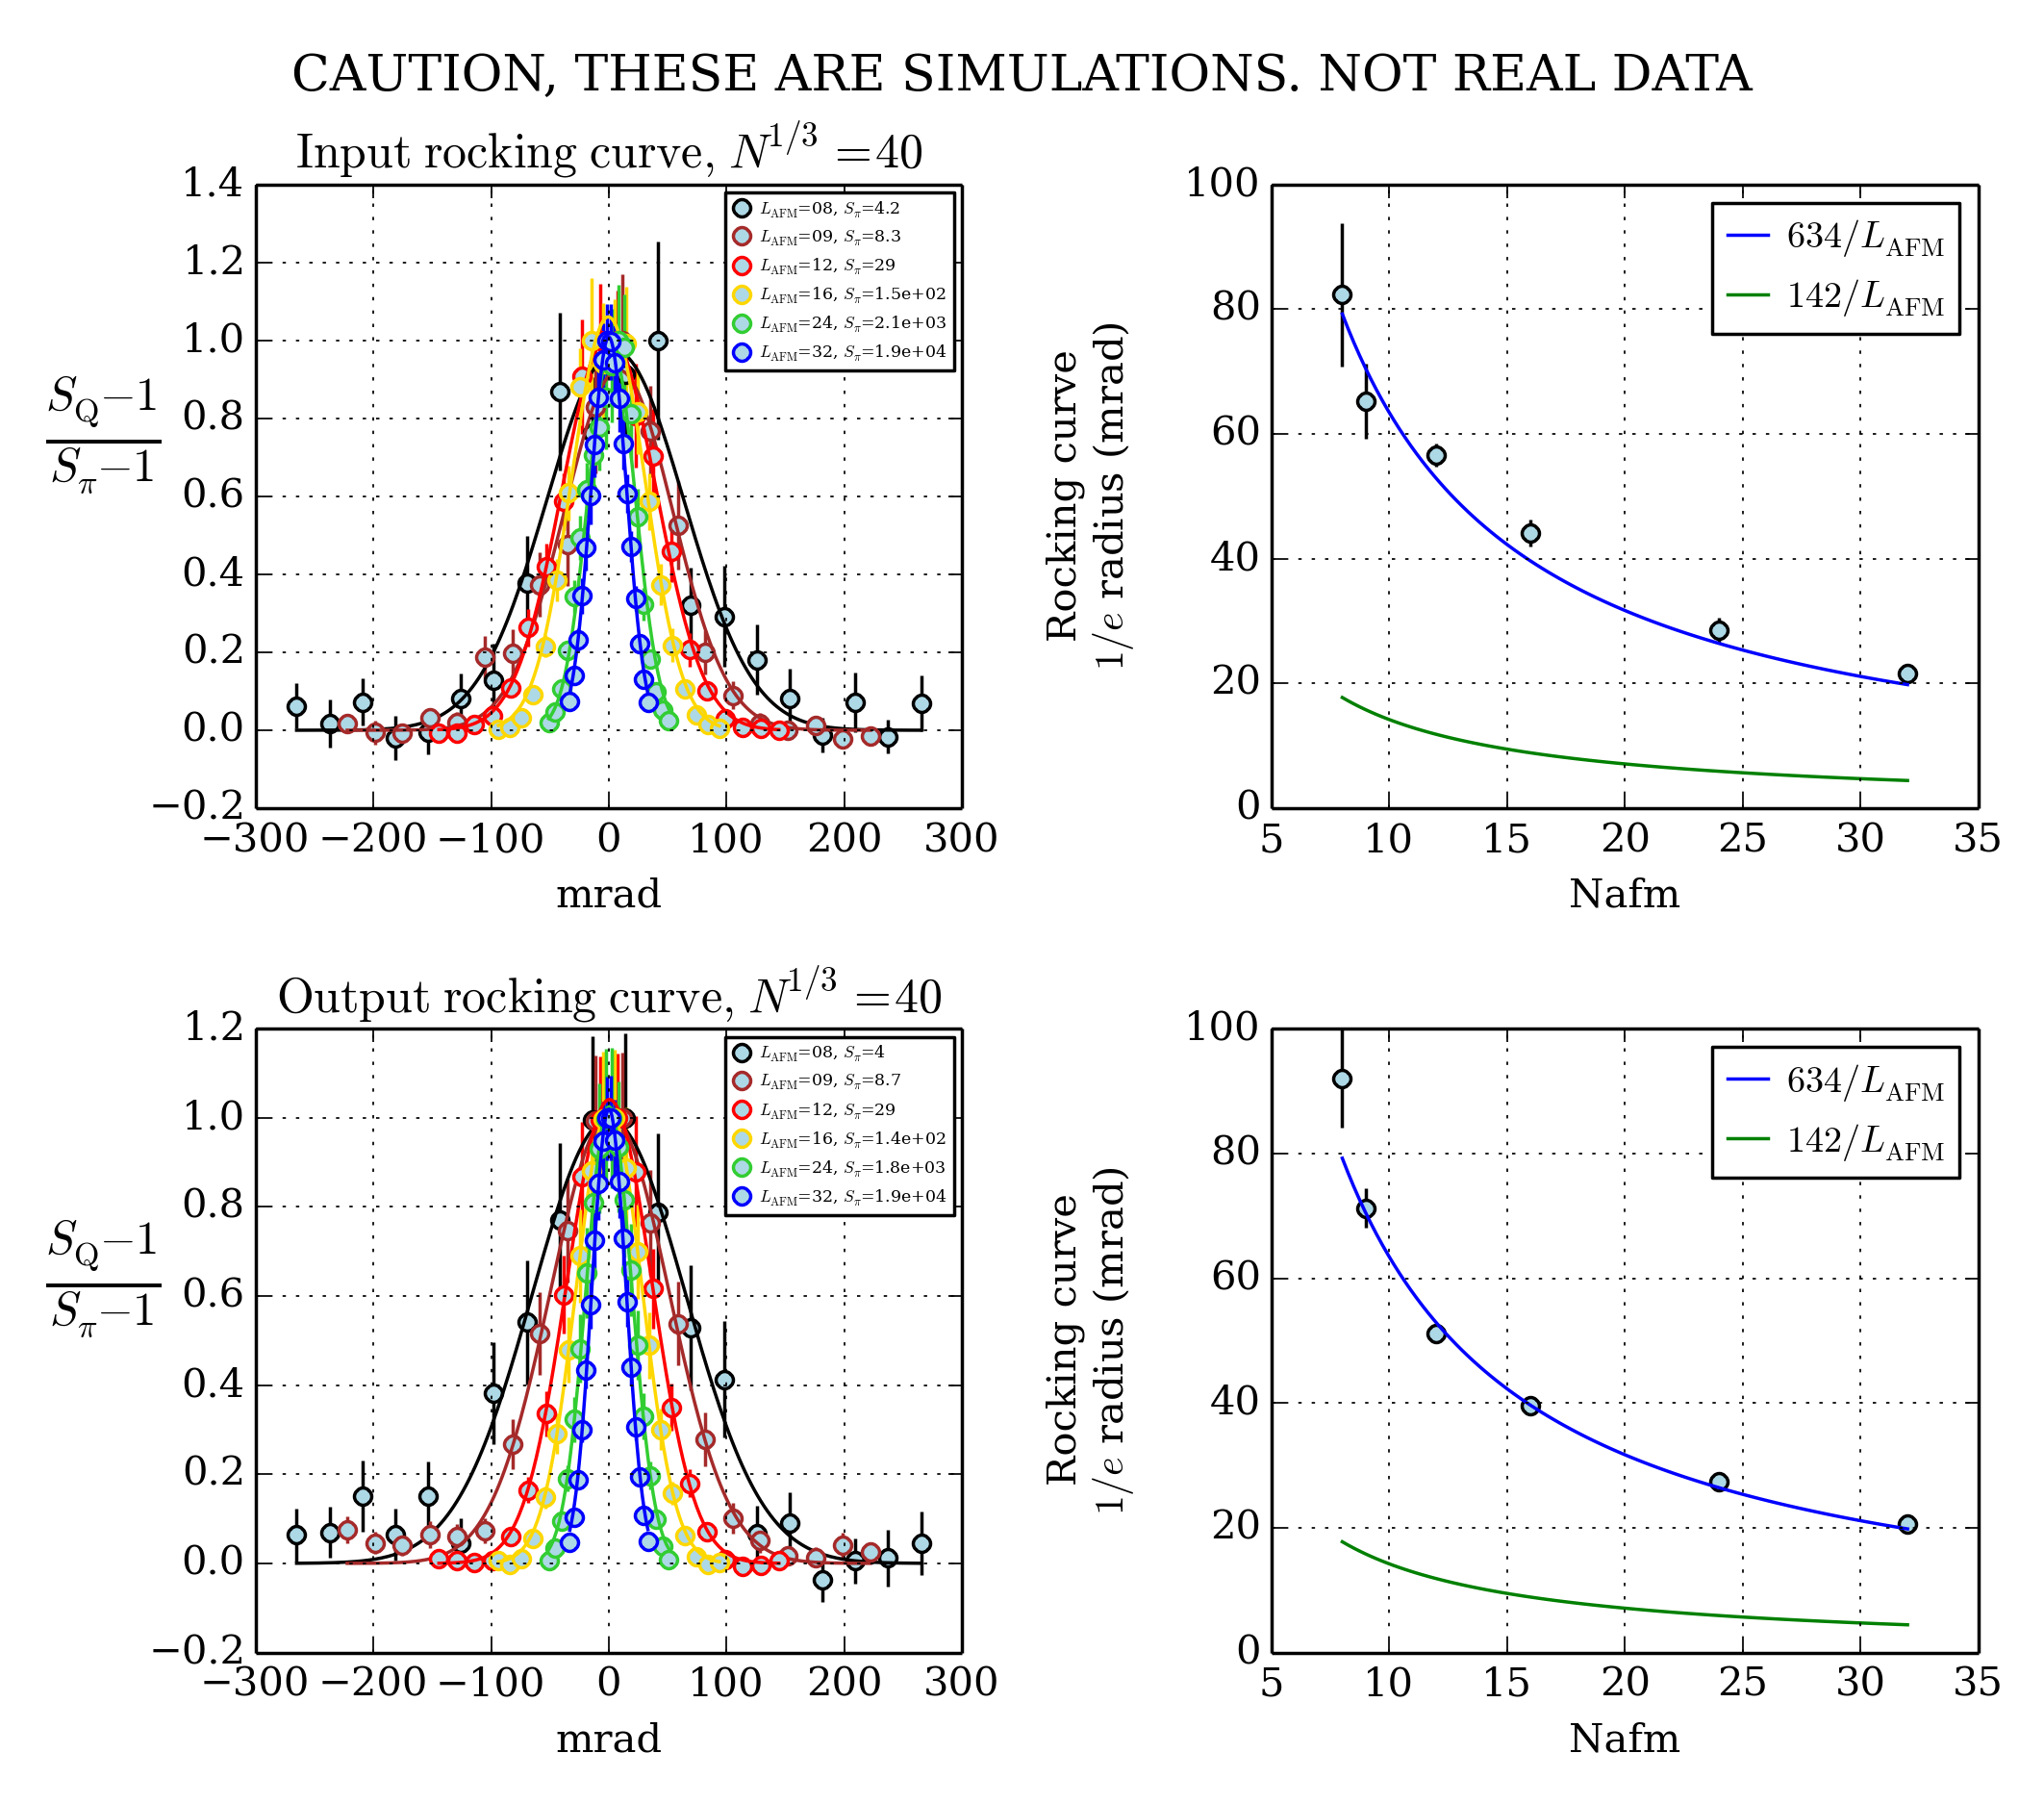
\includegraphics[width=0.6\textwidth]{figures_140308/Rocking_40.png}
\caption[Rocking curve for $N^{1/3}$=40]{\small Rocking curve for $N^{1/3}$=40.
The blue line is the analytical result for the box function correlations and
the green line is the analytical result for the exponentially decaying
correlations.  }
\label{fig:rocking40}
\end{figure}
\begin{figure}[h]
\centering 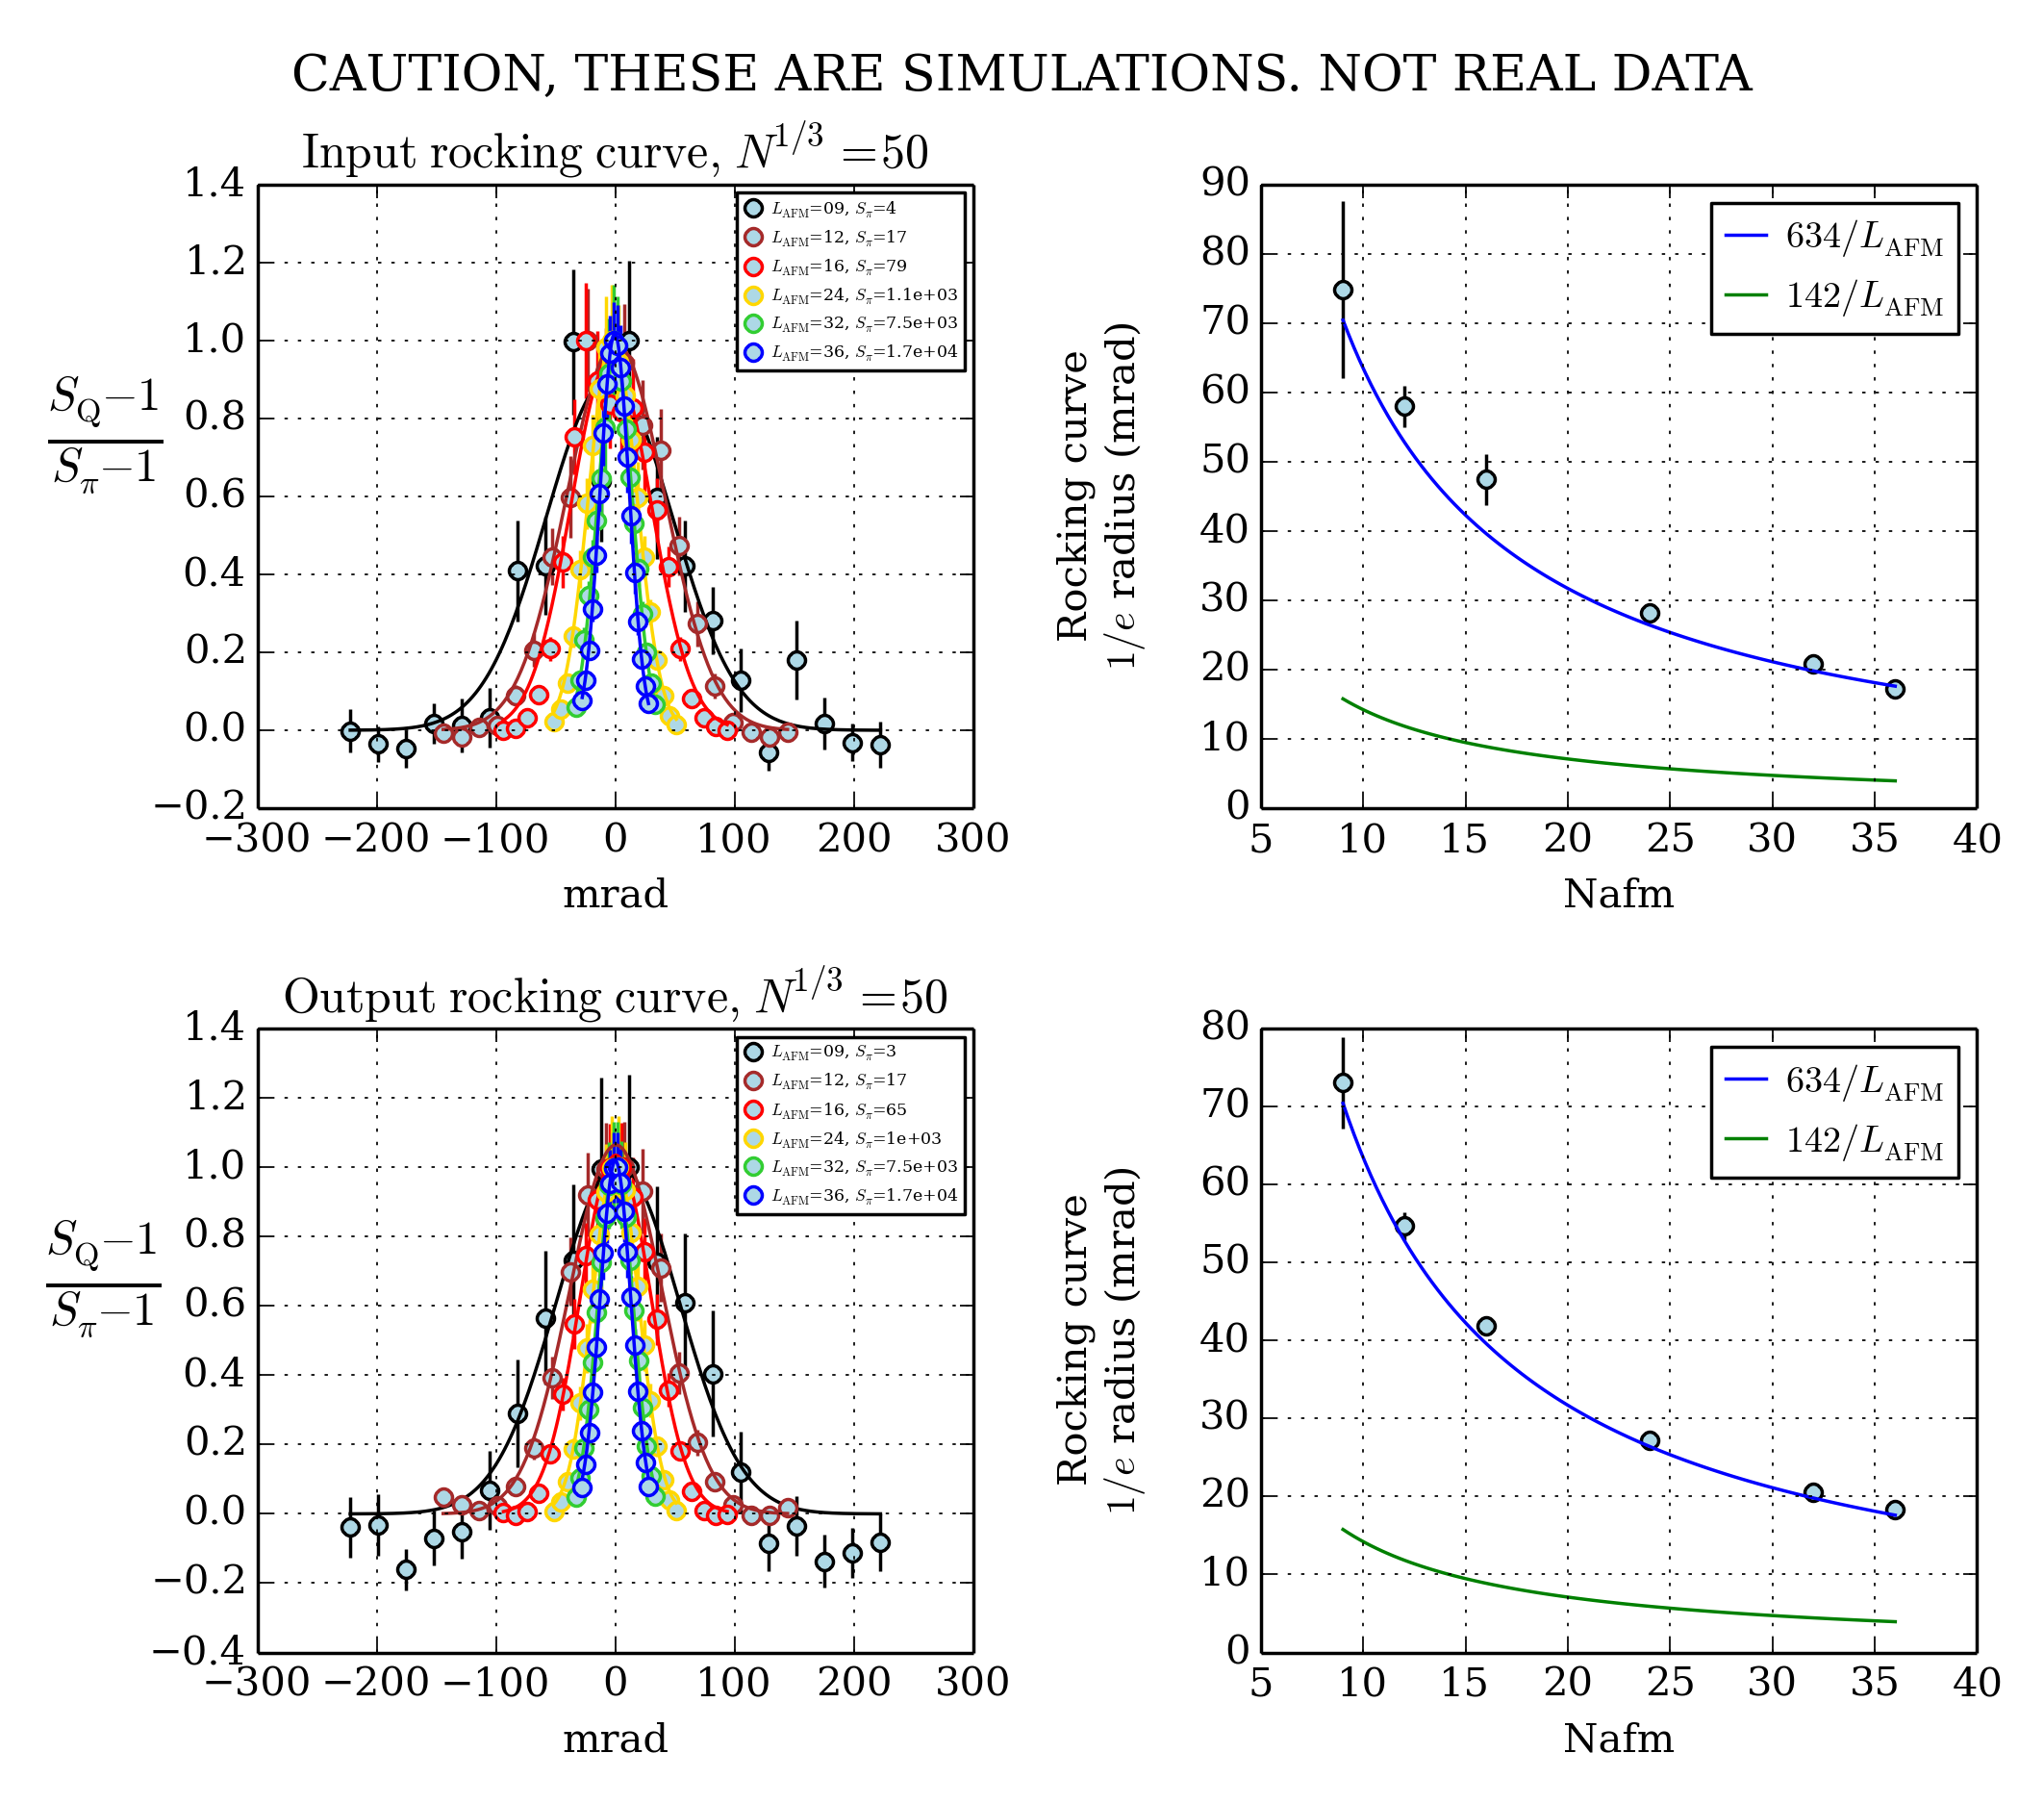
\includegraphics[width=0.6\textwidth]{figures_140308/Rocking_50.png}
\caption[Rocking curve for $N^{1/3}$=50]{\small Rocking curve for $N^{1/3}$=50.
The blue line is the analytical result for the box function correlations and
the green line is the analytical result for the exponentially decaying
correlations.  }
\label{fig:rocking50}
\end{figure}

\subsubsection{Remarks about angular distribution}

We see that the numerical simulations using a random matrix with an AFM core
agree well  with the analytical calculation, which involves taking the 3D
Fourier transform of a box function.  The main approximation done in the
analytical calculation was the replacement of the sum over particles with the
integral over all of space.  Taking the integral over all of space neglects
anything that is happening at the edge of the system.   This is fine for
correlation functions that have a finite support, such as the box or the
exponentially decaying function.   If the system had long range order then an
integral over all of space would diverge. 

It is surprising that the $1/e$ radius of the angular distribution can be so
different for the two different correlation functions studied.  They differ by
a factor of 4. 

\newpage
. 
\newpage

\subsection{Magneto-association and contributions from doubly occupied sites} 

In our experiment we have the possibility to  magneto-associate (MA) the atoms
in doubly occupied sites prior to a measurement of the scattered light.  The
formed molecules  are largely detuned from the probe light and the light that
they scatter is negligible. In this section we study the implications of MA for
the comparison between experimental measurements and the structure factor as
calculated by the theorists. 

We start from Eq.~\ref{eq:iscatt-large-detuning} and will separate the sums
over atoms in singly and doubly occupied sites.  Without carrying out the sums,
Eq.~\ref{eq:iscatt-large-detuning} reads 
\begin{equation}
\begin{split} 
 \Iq 
&  = \frac{ \Iqtof }{N} 
  \left[ 
      4 c \sum_{mn}  
      e^{ i \bv{Q}( \bv{R}_{m} - \bv{R}_{n} ) } 
      S_{zm}S_{zn}
    -  c  \sum_{n} 
  + \sum_{n}  
   \right]  \\ 
\end{split}
\end{equation}

With MA prior to the intensity measurement, there is no contribution to the
scattered light from atoms in doubly occupied sites, so denoting as
$\mathcal{S}$ the set of singly occupied sites, we have 
\begin{equation}
\begin{split} 
 \Iqma  
&  = \frac{ \Iqtof }{N} 
  \left[ 
      4 c \sum_{m\in \mathcal{S}}  
      e^{ i \bv{Q} \bv{R}_{m} } S_{zm} 
      \sum_{n\in \mathcal{S} } 
      e^{ -i \bv{Q} \bv{R}_{n} } S_{zn} 
    -  c  \sum_{n\in \mathcal{S}} 
  + \sum_{n \in \mathcal{S}}  
   \right]  \\ 
&  = \frac{ \Iqtof }{N} 
  \left[ 
      4 c \sum_{m\in \mathcal{S}}  
      e^{ i \bv{Q} \bv{R}_{m} } S_{zm} 
      \sum_{n\in \mathcal{S} } 
      e^{ -i \bv{Q} \bv{R}_{n} } S_{zn} 
    -  c N(1-D)  + N(1-D) 
   \right]  \\ 
\end{split}
\end{equation}
where $D$ is the fraction of atoms in doubly occupied sites.  

Denoting the set of atoms in doubly occupied sites as $\mathcal{D}$, we point
out that 
\begin{equation}
 \sum_{m \in \mathcal{D} }  e^{ \pm i \bv{Q} \bv{R}_{m}} S_{AM} = 0 
\end{equation}
since the contributions cancel out in pairs as $   e^{ \pm i \bv{Q} \bv{R}_{m}}
( +1/2 - 1/2 ) = 0 $.  This allows us to remove the $\in \mathcal{S}$
constraint in the remaining sums: 
\begin{equation}
 \sum_{m \in \mathcal{S} }  e^{ \pm i \bv{Q} \bv{R}_{m}} S_{zm} = 
 \sum_{m}  e^{ \pm i \bv{Q} \bv{R}_{m}} S_{zm}  
\end{equation}

and obtain for the intensity after MA 
\begin{equation}
\begin{split} 
 \Iqma
&  = \frac{ \Iqtof }{N} 
  \left[ 
      4 c \sum_{m}  
      e^{ i \bv{Q} \bv{R}_{m} } S_{zm} 
      \sum_{n } 
      e^{ -i \bv{Q} \bv{R}_{n} } S_{zn} 
    -  c N(1-D)  + N(1-D) 
   \right]  \\ 
&  =  \Iqtof 
  \left[ c S_{\bv{Q}}
    -  c (1-D)  + (1-D) 
   \right]  \\ 
\end{split}
\end{equation}

We introduce the simplifying notation
\begin{equation}
 \frac{  \Iqma } { \Iqtof } \equiv \iqma  
\end{equation}
and solve for the spin structure factor to obtain
\begin{equation}
S_{\bv{Q}} = \frac{1}{c}\left( \iqma  - 1 \right)
             + 1 + \frac{D}{c}(1-c) 
\end{equation}

To measure the fraction of atoms in doubly occupied sites, $D$, we can make a
measurement of the scattered intensity after MA and a large TOF.  Combined with
the TOF measurement without MA we have 
\begin{equation}
  D = 1 - \frac{\Iqmatof }{ \Iqtof } \equiv 1 - \is 
\end{equation} 
giving finally 
\begin{equation}
S_{\bv{Q}} = \frac{\iqma}{c} + \frac{c-1}{c} \is 
\end{equation}

We have taken sets of data where we only record $\Iqmatof$ and $\Iqma$. Under
this conditions we can use the following two equations to solve for the
structure factor
\begin{equation} 
\frac{\Iqma }{\Iqtof}  = cS_{\bv{Q}} - c(1-D) + (1-D)
\ \ \ \ \ \ \ \ \ \ \ 
\frac{ \Iqmatof }{\Iqtof}  =  1 -D 
\end{equation} 
\begin{equation}
S_{\bv{Q}} = \frac{1-D}{c} ( \jqma + c - 1 )  
\ \ \ \ \ \ \ \ \ \ \ 
\jqma \equiv  \frac{\Iqma}{\Iqmatof} 
\end{equation}

We still need knowledge of the double occupancy $D$, so for sets with only
$\Iqmatof$ and $\Iqma$ we have to use $D$ from another data set.

\subsection{Data at short time-of-flight} 

In the above section we considered $\Iqtof$, a measurement of the intensity with
a time-of-flight long enough such that the Debye-Waller factor $e^{-2W}
\rightarrow 0 $.   For some of the data we have taken, the TOF is 6~$\mu$s,
which in some cases is not long enough for the Debye-Waller factor be
negligible.  In this section we look at the determination of $S_{\bv{Q}}$ with
time of flight data for which one cannot assume $e^{-2W} \rightarrow 0 $.  

We recall that the Debye-Waller factor is defined as
\begin{equation}
    e^{-2W} = 
      \prod_{i=x,y,z} e^{ -Q_{i}^{2}\langle r_{i} ^{2} \rangle } 
\end{equation}
where $Q_{i}$ is the $i^{\text{th}}$ component of the momentum transfer $\bv{Q}
= \bv{k}' - \bv{k}$,  with $\bv{k}'$ and $\bv{k}$ the wave vectors of the
outgoing and incoming light respectively.  The time-of-flight dependence of the
Debye-Waller factor is through the expanding size of the atomic wavefunctions.
For an in-situ picture $\langle r_{i}^{2}\rangle$ corresponds to the position
spread of the lattice site's harmonic oscillator ground state.  After the atoms
are released from the lattice the spread of the wavefunction satisfies 
\begin{equation}
\begin{split} 
  \langle r_{i}^{2} \rangle_{t} = &
   \langle r_{i}^{2} \rangle_{0} + 
  \frac{t^{2}}{m^{2}} \langle p_{i}^{2} \rangle_{0} \\
  = &  \langle r_{i}^{2} \rangle_{0} + 
  \frac{t^{2}}{m^{2}} \frac{\hbar^{2}}{4  \langle r_{i}^{2} \rangle_{0} } \\
\end{split}
\end{equation} 

In a harmonic oscillator potential we have 
\begin{equation}
    \langle r^{2} \rangle = \frac{\hbar}{2 m \omega}
\end{equation}
and since in a lattice of depth $V_{0}$ recoils,  $\hbar \omega = 2 E_{R}
\sqrt{V_{0}}$  
\begin{equation}
    \langle r^{2} \rangle = \frac{a^{2}}{ 2 \pi^{2} \sqrt{V_{0}} }
\end{equation}
where $a$ is the lattice spacing. 

We then have for the Debye-Waller factor as a function of time-of-flight
\begin{equation}
\begin{split}
    [e^{-2W}]_{t} = &  
      \prod_{i=x,y,z} \exp\left[  -Q_{i}^{2} 
      \left(  \frac{a^{2}}{ 2 \pi^{2} \sqrt{V_{0}}} 
            + \frac{ h^{2} \sqrt{V_{0}} }{8 a^{2}} 
              \frac{ t^{2}}{m^{2} }\right) \right] \\
    =& [e^{-2W}]_{0} \prod_{i=x,y,z} \exp\left[  -Q_{i}^{2} 
            \frac{ h^{2} \sqrt{V_{0}} }{8 a^{2}} 
              \frac{ t^{2}}{m^{2} } \right] \\
    =& [e^{-2W}]_{0} \prod_{i=x,y,z} \exp\left[ -\frac{\sqrt{V_{0}}}{2}
           \left( \frac{ Q_{i} h }{2 m a  } \right)^{2}  t^{2}   \right] \\
    =& [e^{-2W}]_{0} \exp\left[ -\frac{\sqrt{V_{0}}}{2}
           \left( \frac{ |\bv{Q}| h }{2 m a  } \right)^{2}  t^{2}   \right] \\
\end{split}
\end{equation}

We now define the time dependent correction factor 
\begin{equation}
   c(t) =   \frac{ [e^{-2W}]_{t} 4 \Delta^{2}  } 
           {4 \Delta^{2} + 2 \iisat }  
\end{equation}
The measured intensity after time-of-flight $t$ is 
\begin{equation}
\begin{split} 
 \frac{\Iq(t)}{\Iqtof} 
&  = c(t) ( S_{\bv{Q}} - 1 ) + 1 
\end{split}
\end{equation}
Consider two measurements, one at $t=0$, the other one at $t=T$,
\begin{equation}
 \frac{ \Iq(t=0) }{\Iqtof} =  c(0)( S_{\bv{Q}} -1) + 1 
 \ \ \ \ \ \ \ \ \ \ 
  \frac{ \Iq(t=T) }{\Iqtof} =  c(T)( S_{\bv{Q}} -1) + 1 
\end{equation}
Their ratio is
\begin{equation} 
 \frac{ \Iq(t=0)}{ \Iq(t=T)} = 
 \frac{ c(0)( S_{\bv{Q}} - 1 ) + 1}{ c(T)( S_{\bv{Q}} - 1) + 1} 
      \equiv  \iqT 
\end{equation}
which can be solved to give
\begin{equation} 
  S_{\bv{Q}} = \frac{ 1 - c(0) - \iqT( 1- c(T))}
                    { \iqT c(T) - c(0) } 
\end{equation}

\subsection{Simultaneous measurement of the structure factor for two different
values of $\bv{Q}$}

In the sections above we have shown how to measure the spin structure factor
$S_{\bv{Q}}$  by measuring the scattered intensity in-situ and after
time-of-flight.  An issue that arises with this measurement is that the in-situ
and TOF measurements require two different realizations of the experiment.  

In our setup we have the possibility of measuring the scattered intensity at
two different output angles.  One of the angles corresponds to a momentum
transfer $\bv{Q} = \frac{2\pi}{a} ( \frac{1}{2}\, \frac{1}{2}\, \frac{1}{2} )
\equiv \bv{\pi}$,  which offers the possibility of measuring the staggered
magnetization of the system, i.e. the degree of antiferromagnetic ordering.
The other angle corresponds to a momentum transfer $\bv{Q} = \frac{2\pi}{a}(
0.4,\, -0.1,\, -0.04 ) \equiv \bv{\theta}$.  The structure factor can also be
measured at this value of $\bv{Q}$ and compared with theoretical calculations.
Since this momentum transfer does not measure the staggered magnetization 
it may be used as a normalization for the measurement at $\bv{Q}=\bv{\pi}$

For the measurements at $\bv{\pi}$ and $\bv{\theta}$ we have (without
magneto-association)
\begin{equation}
   S_{\bv{\pi}} = (i_{\bv{\pi}} - 1 + c_{\bv{\pi}})/c_{\bv{\pi}}
  \ \ \ \ \ \ \ \ \ \ 
   S_{\bv{\theta}} = (i_{\bv{\theta}} - 1 + c_{\bv{\theta}})/c_{\bv{\theta}}
\end{equation}
\begin{equation}
  \frac{ S_{\bv{\pi}} }{ S_{\bv{\theta}}} = 
  \frac{ i_{\bv{\pi}} - 1 + c_{\bv{\pi}} }{ i_{\bv{\theta}} - 1 + c_{\bv{\theta}} } 
  \left( \frac{ c_{\bv{\theta}} }{ c_{\bv{\pi}}} \right)
\end{equation}
To make use of the simultaneous measurement of $I$ at $\bv{Q}= \bv{\pi},
\bv{\theta}$ we define 
\begin{equation}
  \left. 
  \left( \frac{ I_{\bv{\pi}} }{ I_{\bv{\theta}}} \right)  \middle/  
  \left( \frac{ \Itof{\pi} }{ \Itof{\theta} } \right)  
  \right.  \equiv \ipith
\end{equation}
The advantage here is that the ratio $\frac{ \Itof{\pi} }{ \Itof{\theta} }$ is
determined only by the solid angle and responsivity of the cameras.  One can
calibrate this ratio beforehand and then, using the calibration, get a single
shot measurement of $\ipith$

The ratio of the structure factors at $\bv{\pi}$ and $\bv{\theta}$ is given by
\begin{equation}
  \frac{ S_{\bv{\pi}} }{ S_{\bv{\theta}} } = 
  \frac{ \ipith  - ( 1 - c_{\bv{\pi}} )/i_{\bv{\theta}} }
        { 1 - (1 - c_{\bv{\theta}})/i_{\bv{\theta}} } 
  \left( \frac{ c_{\bv{\theta}} }{ c_{\bv{\pi}}} \right)
\end{equation}

If our correction factors were close to 1 we could obtain the ratio of
structure factors in one shot as 
\begin{equation}
  \frac{ S_{\bv{\pi}} }{ S_{\bv{\theta}} } \approx \ipith
\end{equation}
Besides being able to get this in one shot it has the added advantage that any
common mode noise between the two cameras gets canceled out, this includes
atom number fluctuations and fluctuations in the intensity or polarization of
the probe light.  Unfortunately with our $50\,E_{R}$ lattice and $\iisat=15$ we
have 
\begin{equation}
  c_{\bv{\pi}} =  0.686
 \ \ \ \ \ \ \ \ \ \ 
  c_{\bv{\theta}} = 0.805 
\end{equation} 
which results in a non-negligible correction that depend on $i_{\bv{\theta}}$.
In our case this is not such a drawback because the camera located at
$\bv{\theta}$ has a solid angle that is 10 time larger than the camera located
at $\bv{\pi}$.  

We can also obtain formulas for the ratio $S_{\bv{\pi}}/S_{\bv{\theta}}$ under
the conditions described in the two previous sections.  

In the case where the time-of-flight is not large enough for
$e^{-2W}\rightarrow 0$ we have the formula
\begin{equation}
   \frac{ S_{\bv{\pi}}}{ S_{\bv{\theta}}} = 
   \frac{ [1-c_{\bv{\pi}}(0)]/ \iT{\theta}   
         - \iT{(\pi/\theta)} [1-c_{\bv{\pi}}(T) ] }
        {  [1-c_{\bv{\theta}}(0)]/\iT{\theta}  - [1-c_{\bv{\theta}}(T)]  }
   \frac{ c_{\bv{\theta}}(T) - c_{\bv{\theta}}(0)/ \iT{\theta}  } 
        { \iT{(\pi/\theta)}  c_{\bv{\pi}}(T) 
          - c_{\bv{\pi}}(0)/ \iT{\theta} } 
\end{equation}

If the in-situ intensity is measured after magneto-association we have 
\begin{equation}
   \frac{ S_{\bv{\pi}}}{ S_{\bv{\theta}}} = 
   \frac{ c_{\bv{\theta}} } { c_{\bv{\pi}} } 
   \frac{  \ima{(\pi/\theta)} 
               + (c_{\bv{\pi}} - 1 ) (1-D) / \ima{\theta} } 
        {   1 
               + (c_{\bv{\theta}} - 1 ) (1-D) / \ima{\theta} } 
\end{equation}

If both the in-situ and TOF intensity are measured after magneto-association we
have
\begin{equation}
    \frac{ S_{\bv{\pi}}}{ S_{\bv{\theta}}} = 
    \frac{ c_{\bv{\theta}} } { c_{\bv{\pi}} } 
    \frac{ \jma{(\pi/\theta)}  + (c_{\bv{\pi}} - 1 ) / \jma{\theta}  }
         { 1 +  (c_{\bv{\theta}} - 1 ) \jma{\theta} } 
\end{equation}
   
\newpage
 
\subsection{Summary of structure factor formulas }    

Below we show the different ways to calculate the structure factor from our
measurements.  A correction factor, $c_{\bv{Q}}$ appears in the formulas to
account for the non-unity Debye-Waller factor in the lattice and also for the
intensity of the probe beam.  The formula for the correction factor is 
\begin{equation} 
      c_{\bv{Q}} = \frac{ e^{-2W}4 \Delta^{2}  } 
           {(4 \Delta^{2} + 2 \iisat) }
\end{equation} 
The Debye-Waller factor, $e^{-2W}$ depends on the momentum transfer $\bv{Q}$.
In our experiment the corrections are significant.  The largest lattice depth
we can reach is $50\,E_{R}$, and in order to moderately overcome the dark noise
of the camera we use a probe intensity of $I_{p}=15\,\isat$.   This results in
the following values for $\bv{\pi}$ and $\bv{\theta}$, the two values of the
momentum transfer that we have access to:
\begin{equation}
\bv{\pi} = \frac{2\pi}{a} ( 0.5,\, 0.5,\, 0.5 ) 
\ \ \ \ \ \ \ \ \ \
 \bv{\theta} = \frac{2\pi}{a}( 0.4,\, -0.1,\, -0.04 )
\end{equation}
\begin{equation}
  e^{-2W}_{\bv{\pi}} =  0.81
 \ \ \ \ \ \ \ \ \ \ 
  e^{-2W}_{\bv{\theta}} = 0.95
 \ \ \ \ \ \ \ \ \ \ 
  1  +   \frac{\iisat}{2\Delta^{2} } =  1.18  
\end{equation}
\begin{equation}
  c_{\bv{\pi}} =  0.686
 \ \ \ \ \ \ \ \ \ \ 
  c_{\bv{\theta}} = 0.805 
\end{equation}

The duration of our scattering pulse is 1.7\,$\mu$s, and we scatter on the
average 4.7 photons per atom.   At our lattice depth of 50\,$E_{R}$, the square
of the Lamb-Dicke parameter is $\eta_{LD}^{2} = 0.07$ which means that we can
approximately scatter 14 photons per atom before we kick the atom into an
excited band.  At the moment we have not introduced corrections for atoms
recoiling into excited bands during the measurement. 

In the latest data that we have taken at 5.5\,$E_{R}$ as a function of $U/t$, we
always do a magneto-association sweep before the in-situ picture.   We also
take time-of-flight pictures with and without magneto-association.  The
following table lists the quantities that we measure 

\renewcommand{\arraystretch}{1.5} 
\begin{tabular}{ l | p{15cm}  }
  \multicolumn{2}{l}{ \large \bf CCD measurements: } \\ 
  \noalign{\smallskip} 
%  \Iq    & In-situ intensity measured at momentum transfer $\bv{Q}$  \\ \hline
  \Iqma  & In-situ intensity measured at momentum transfer $\bv{Q}$ after 
           magneto-association of doubly occupied sites into molecules. 
           Molecules are dark to the probe light.  
               \\ \hline
  \Iqtof & Time-of-flight intensity measured at momentum transfer $\bv{Q}$. 
           We use TOF = 10\,$\mu$s.  \\ \hline
  \Iqmatof & Time-of-flight intensity measured at momentum transfer $\bv{Q}$ after 
           magneto-association of doubly occupied sites into molecules. 
           Molecules are dark to the probe light.
\end{tabular}

\vspace{1em}

\onehalfspacing

\renewcommand{\arraystretch}{2.0} 
\begin{tabular}{ l | p{15cm}  }
  \multicolumn{2}{l}{ \large \bf Ratios of CCD measurements: } \\  
  \noalign{\smallskip} 
%  $\iq$    &  $\frac{\Iq}{\Iqtof}$   \\ \hline 
  $\iqma$  &  $\frac{\Iqma}{\Iqtof}$ \ \ For a given $U/t$ the set of $\Iqma$\ is 
              averaged and the set of $\Iqtof$\ is averaged, then the ratio is 
              calculated.     \\ \hline
%  $\jqma$  &  $\frac{\Iqma}{\Iqmatof}$ \\ \hline
  $\is$    &  $\frac{\Iqmatof}{\Iqtof} \equiv 1-D $ , where $D$ is
              the double occupancy.  For a given $U/t$ the set of $\Iqmatof$\
              is averaged and the set of $\Iqtof$\ is averaged, then the 
              ratio is calculated. \\ \hline
%  $D$      &  $ 1 - \is$ \ \  This is the double occupancy. \\ \hline
  $\ima{(\pi/\theta)}$ &   
  $\left. 
  \left( \frac{ \Ima{\pi} }{ \Ima{\theta} } \right)  \middle/  
  \left( \frac{ \Itof{\pi} }{ \Itof{\theta} } \right)  
  \right. $ \ \ For a given $U/t$ the set of
  $\frac{ \Ima{\pi} }{ \Ima{\theta} }$ is averaged and the 
  set of $\frac{ \Itof{\pi} }{ \Itof{\theta} }$ is averaged, then
  the ratio is calculated.  \\ \hline
  $\fma{(\pi/\theta)}$ &  
  $\left. 
  \left( \frac{ \Ima{\pi} }{ \Ima{\theta} } \right)  \middle/ 
  \overline{ 
  \left( \frac{ \Itof{\pi} }{ \Itof{\theta} } \right)}  
  \right. $ \ \ For a given $U/t$ the set of
  $\frac{ \Ima{\pi} }{ \Ima{\theta} }$ is averaged.  The 
  set of $\frac{ \Itof{\pi} }{ \Itof{\theta} }$ is averaged for all data
  at any $U/t$ value.  This can be done since the TOF ratio depends only on 
  the solid angle and the responsivity of the CCDs.   \\ \hline
\end{tabular}

\singlespacing

\vspace{1em}


We the use the quantities in the table above to determine the two structure
factors and their ratio in the following ways: 
 
\renewcommand{\arraystretch}{2.0} 
\begin{tabular}{ l | l | p{6cm} | p{8.5cm}  }
  \multicolumn{4}{l}{ \large \bf Structure factor formulas relevant for latest data  } \\  
  \noalign{\smallskip}  
  0. &
  $S_{\bv{\pi}}/S_{\bv{\theta}}$ &
   { \Large
   $\frac{ c_{\bv{\theta}} } { c_{\bv{\pi}} } 
   \frac{  \ima{(\pi/\theta)} 
               + (c_{\bv{\pi}} - 1 ) (1-D) / \ima{\theta} } 
        {   1 
               + (c_{\bv{\theta}} - 1 ) (1-D) / \ima{\theta} } $ }
         & $\ima{(\pi/\theta)}$\ is used.  \\ \hline 
  1. &
  $S_{\bv{\theta}}$  & $\frac{\ima{\theta}}{c_{\bv{\theta}}} 
      + \frac{ c_{\bv{\theta}} -1 }{c_{\bv{\theta}}}(1-D)$ 
                & For the determination of $D$ we use $D = 1 - \is$  
                  \\ \hline
  2. &
  $S_{\bv{\pi}}$  & $\frac{\ima{\pi}}{c_{\bv{\pi}}} 
      + \frac{ c_{\bv{\pi}} -1 }{c_{\bv{\pi}}}(1-D)$ 
                & For the determination of $D$ we use $D = 1 - \is$  
                  \\ \hline
  3. &
  $S_{\bv{\pi}}/S_{\bv{\theta}}$ &
  { \Large 
   $\frac{ c_{\bv{\theta}} } { c_{\bv{\pi}} } 
   \frac{  \fma{(\pi/\theta)} 
               + (c_{\bv{\pi}} - 1 ) (1-D) / \ima{\theta} } 
        {   1 
               + (c_{\bv{\theta}} - 1 ) (1-D) / \ima{\theta} } $ } 
         & $\fma{(\pi/\theta)}$\ is used.
           This means that we use the calibration of the ratio of the two 
           cameras, which leads to an improvement in the signal to noise ratio
           because common mode noise between the two cameras cancels out. 
            \\ \hline
  5. &
  $S_{\bv{\pi}}$  & $\frac{S_{\pi}}{S_{\theta}} S_{\theta}$ & 
           The results of 1. and 3. are combined to obtain $S_{\bv{\pi}}$.    
\end{tabular}

%%%\renewcommand{\arraystretch}{2.0} 
%%%\begin{tabular}{ l | p{5cm} | p{9.5cm}  }
%%%  \multicolumn{3}{l}{ \large \bf General case structure factor formulas: } \\  
%%%  \noalign{\smallskip} 
%%%  $S_{\bv{Q}}$  & $1+(\iq - 1)/c_{\bv{Q}} $  
%%%                & For data without magneto-association \\ \hline
%%%  $S_{\bv{\pi}}/S_{\bv{\theta}}$ & 
%%%       $\frac{ \ipith  - ( 1 - c_{\bv{\pi}} )/i_{\bv{\theta}} }
%%%              { 1 - (1 - c_{\bv{\theta}})/i_{\bv{\theta}} } 
%%%        \left( \frac{ c_{\bv{\theta}} }{ c_{\bv{\pi}}} \right) $
%%%         &  For data without magneto-association, to obtain the ratio
%%%            of the structure factors.  \\ \hline
%%%  $S_{\bv{Q}}$  & $\frac{\iqma}{c_{\bv{Q}}} 
%%%      + \frac{ c_{\bv{Q}} -1 }{c_{\bv{Q}}}(1-D)$ 
%%%                & For data with MA in-situ but no MA in time-of-flight. 
%%%                  Requires independent knowledge of $D$ for the correction. 
%%%                  \\ \hline
%%%  $S_{\bv{\pi}}/S_{\bv{\theta}}$ & 
%%%   $\frac{ c_{\bv{\theta}} } { c_{\bv{\pi}} } 
%%%   \frac{  \ima{(\pi/\theta)} 
%%%               + (c_{\bv{\pi}} - 1 ) (1-D) / \ima{\theta} } 
%%%        {   1 
%%%               + (c_{\bv{\theta}} - 1 ) (1-D) / \ima{\theta} } $
%%%         & For data with MA in-situ but no MA in time-of-flight. 
%%%           To obtain the ratio of the structure factors.\\ \hline
%%%  $S_{\bv{Q}}$  & $\frac{1-D}{c_{\bv{Q}}}( \jqma + c_{\bv{Q}} -1 ) $ 
%%%                & For data with MA in-situ and  MA in time-of-flight.
%%%                  Requires independent knowledge of $D$ for the correction.
%%%                  \\ \hline
%%%  $S_{\bv{\pi}}/S_{\bv{\theta}}$ & 
%%%    $\frac{ c_{\bv{\theta}} } { c_{\bv{\pi}} } 
%%%    \frac{ \jma{(\pi/\theta)}  + (c_{\bv{\pi}} - 1 ) / \jma{\theta}  }
%%%         { 1 +  (c_{\bv{\theta}} - 1 ) \jma{\theta} } $
%%%         & For data with MA in-situ and MA in time-of-flight. 
%%%           To obtain the ratio of the structure factors. \\ \hline
%%%\end{tabular}

In the data plot shown below each panel has a number on the top left corner
indicating which formula is used to obtain the data.  

{\centering
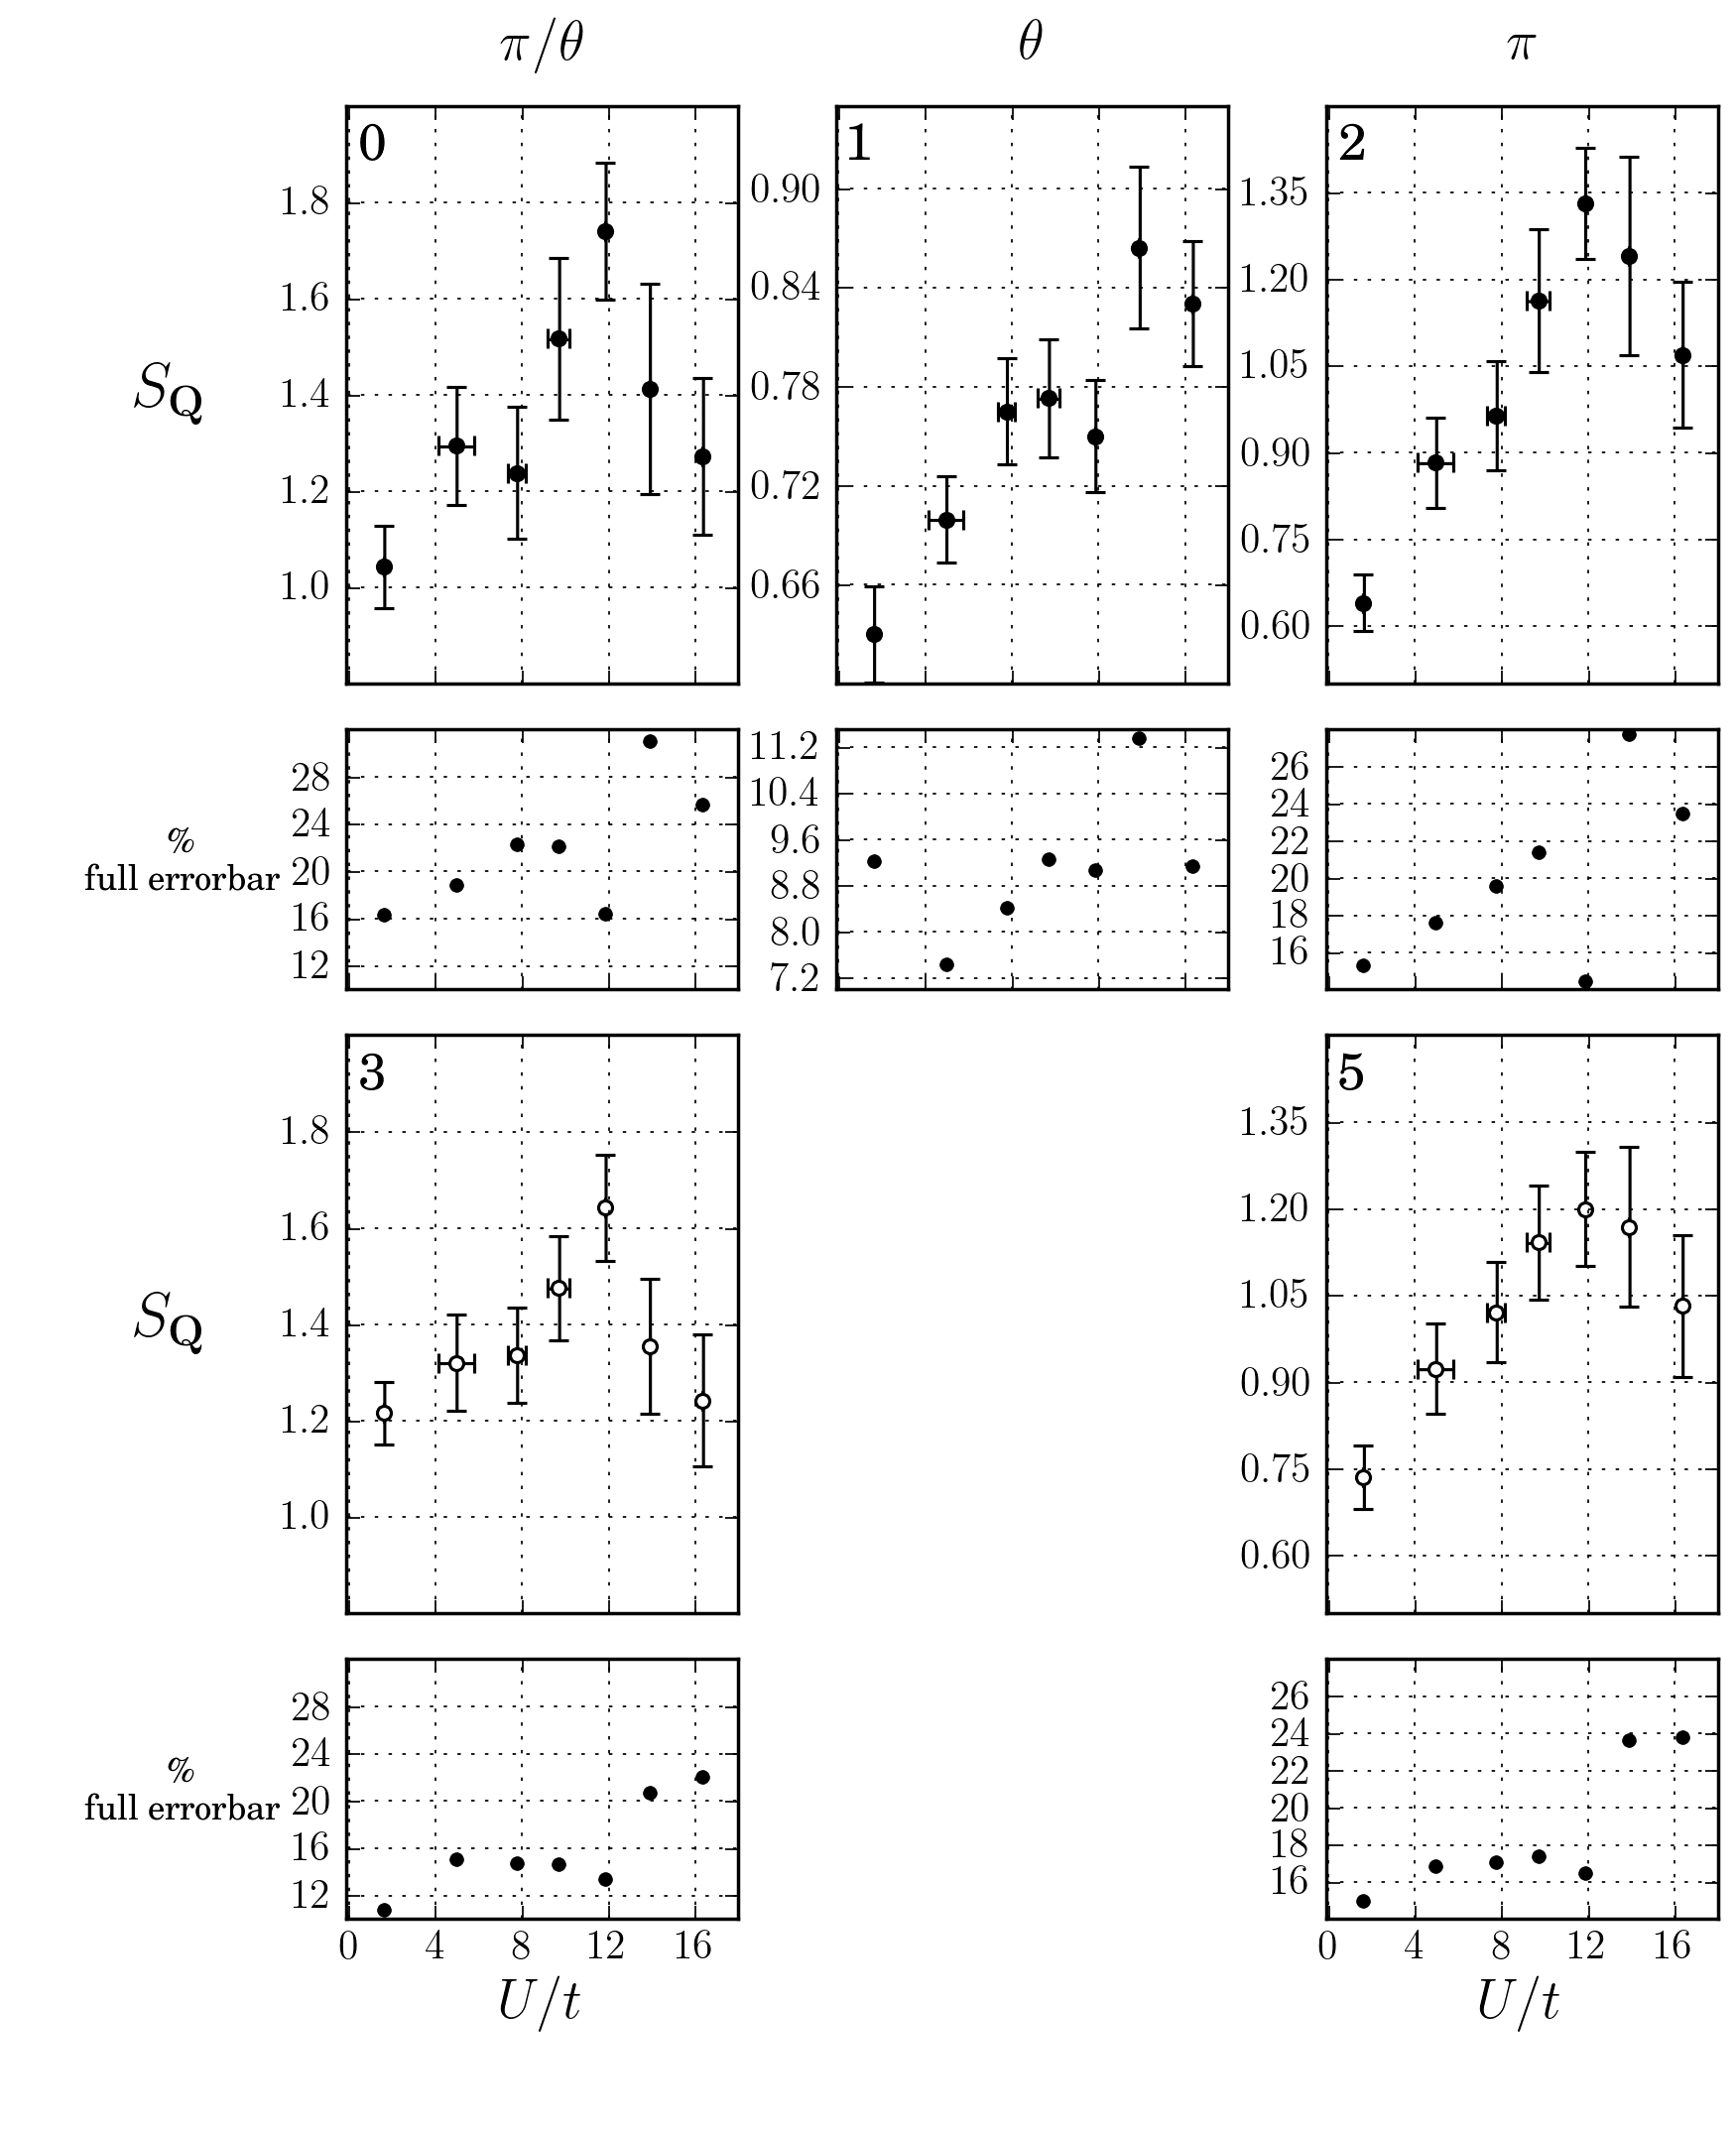
\includegraphics[width=0.9\textwidth]{figures_140128/sdat_average_m.png}}


\subsection{Comments} 

The first row and the third row of the plot shown above involve two different
ways to get to the structure factor from our data.   They are pretty close to
each other within error bars but not fully consistent.   We think that the most
direct way to get to $S_{\bv{\pi}}$ is in the first row.   The most direct way
to get to the ratio $S_{\bv{\pi}}/S_{\bv{\theta}}$ is in the third row, since
it uses the calibrated ratio $\fma{(\pi/\theta)}$ which only depends on the
solid angle and responsivity of the cameras.  



\section{Sample inhomogeneity} 


The Quantum Monte Carlo (QMC) calculations done by the theorists in our
collaboration are for systems with uniform filling, and at a fixed value of the
interaction strength $U/t$. Our sample is far from these uniform conditions.
Since it is a trapped finite sample, the filling (density) goes all the way
down to zero.  Typically, optical lattices are realized with laser beams that
have large beam waists, so the parameters $U$ and $t$ have a negligible
variation over the size of the sample.  In our experiment we used a beam waist
($\approx 45\,\mu\text{m}$) which is comparable to the size of the sample
($1/e$ radius of $\approx 20\,\mu\text{m}$).   For this reason we have a strong
variation of $U$ and $t$ over the size of the sample.  In our system, as you
move from the center to the outside of the atom cloud the lattice gets
shallower, which results in reduced $U$ and increased $t$.   The Hubbard
interaction strength $U/t$ thus suffers from both numerator and denominator
which results in a significant variation of $U/t$ over the cloud. 

The motivation for reducing $U$ and increasing $t$ in length scales comparable
with the sample is such that there may be entropy redistribution to the edges
of the cloud.  Near the edges the system has a larger entropy capacity due to
the lower filling there. Additionally,  since towards the edge the lattice is
shallower, elastic collisions may lead to evaporation of the particles which
may resulting in cooling of the system. 

To incorporate the effects of inhomogeneity in the comparison between QMC and
our measurements we will divide our sample into five bins, each with equal
number of particles and then get the values of the filling $n$ and the Hubbard
parameters $U$ and $t$ for each of the bins. QMC
calculations of the structure factor can be performed for each bin and then
averaged before comparing with the experimental results. 

To calculate the average value of the parameters in each bin we need knowledge
of the density profile of our cloud, as well as knowledge of our optical
lattice potential. The potential can be calculated from the calibrated beam
waists and power of our optical lattice beams.   

For the density profile we can perform in-situ phase-contrast images of the
atom cloud.  Alternatively,  with our known atom number and the calculated
potential we can use a thermodynamic model of the system to calculate the
expected density distribution.   The thermodynamic model we use is the high
temperature series expansion up to second order in $T/t$, which can be
calculated readily and is accurate down to about $T/t \approx 1.8$.   To avoid
complications with the repeatability in the realization of a certain density
distribution we choose this second alternative.  We feed into the model the
atom number measured in the experiment. As a sanity check we can plot a
particular realization of the density distribution and compare it with the
calculation from the thermodynamic model.  We can check if the peak density,
double occupancy, and cloud size roughly agree with the model. 

 
In Fig.~\ref{fig:in-situ-density} we show a plot of the in-situ density
distribution measured using phase-contrast imaging in a 5.5\,$E_{R}$ lattice
with 3.0\,$E_{R}$ of green compensation.
\begin{figure}
\centering 
%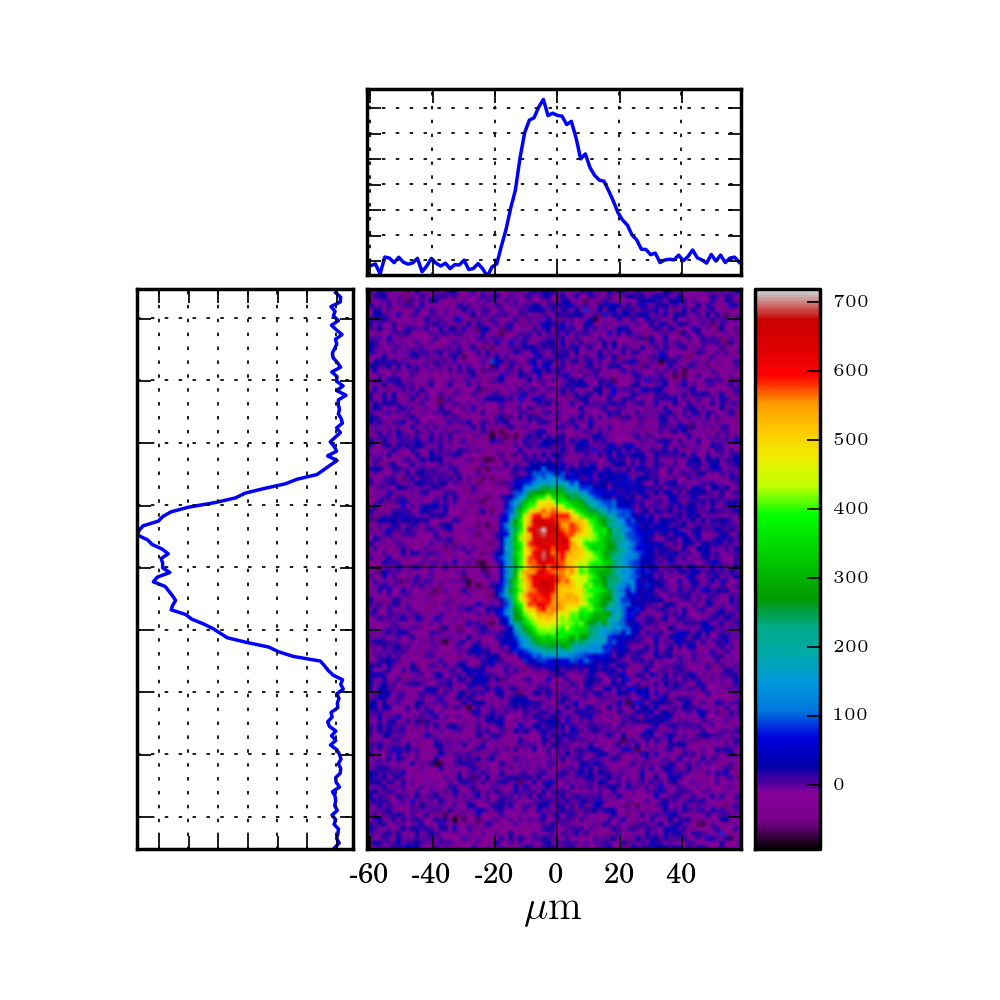
\includegraphics[width=0.5\textwidth]{figures_140129/densityInspec_7776.png}
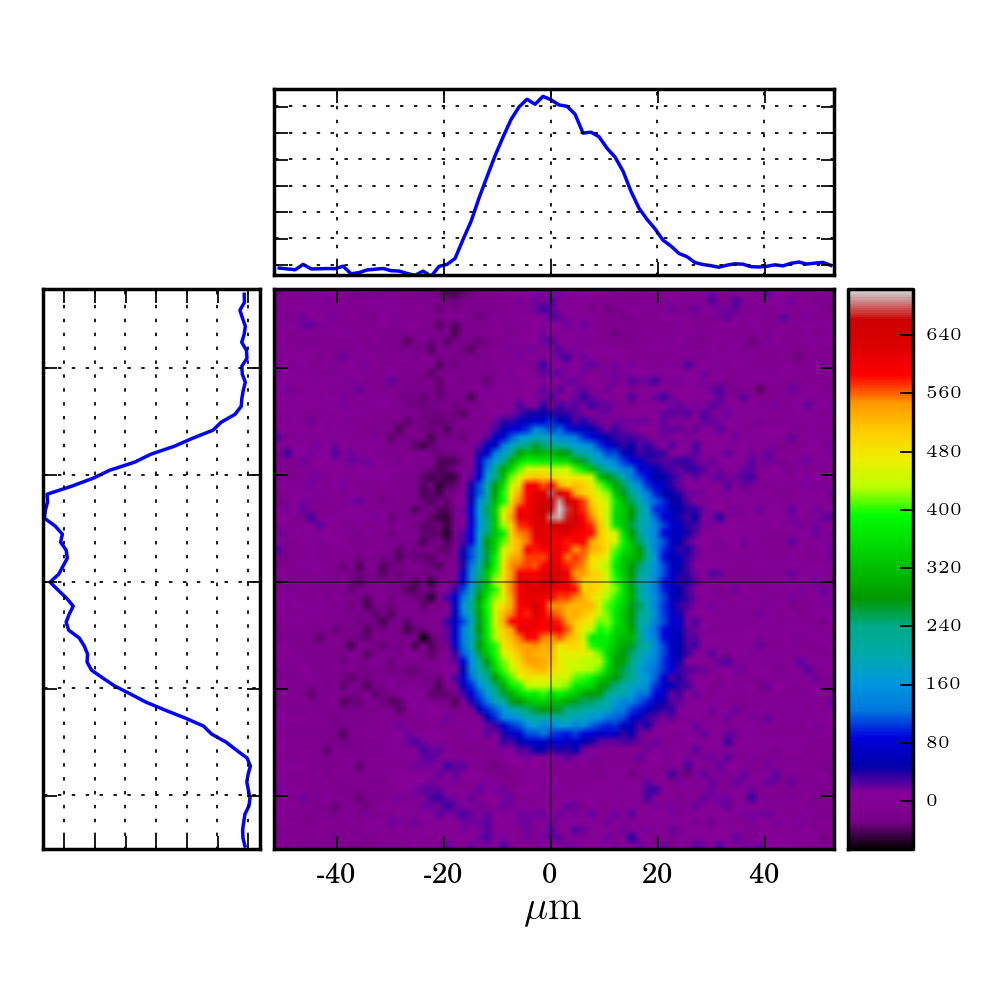
\includegraphics[width=0.4\textwidth]{figures_140130/densityinspec_380a0_avg.png}
\caption[In-situ column density distribution]{\small In-situ column density
distribution in a 5.5\,$E_{R}$ lattice with 3\,$E_{R}$ of green compensation.
} \label{fig:in-situ-density}
\end{figure}
It can be seen that the distribution is not spherically symmetric and that it is some irregularities.  The $1/e$ sizes are 14~$\mu$m
and 23~$\mu$m.  The number of atoms in the cloud is 330,000.  The density at
the peak is estimated from the number and the cloud sizes to be
6.45e12~$\mathrm{cm}^{-3}$ which corresponds to 0.97 atoms per site.   The
image shown was taken at a scattering length of 380~$a_{0}$.

If we put 330,000 atoms into the model we obtain the results shown in
Fig.~\ref{fig:thermo-green} for various values of the green compensation.  
\begin{figure}
\centering 
%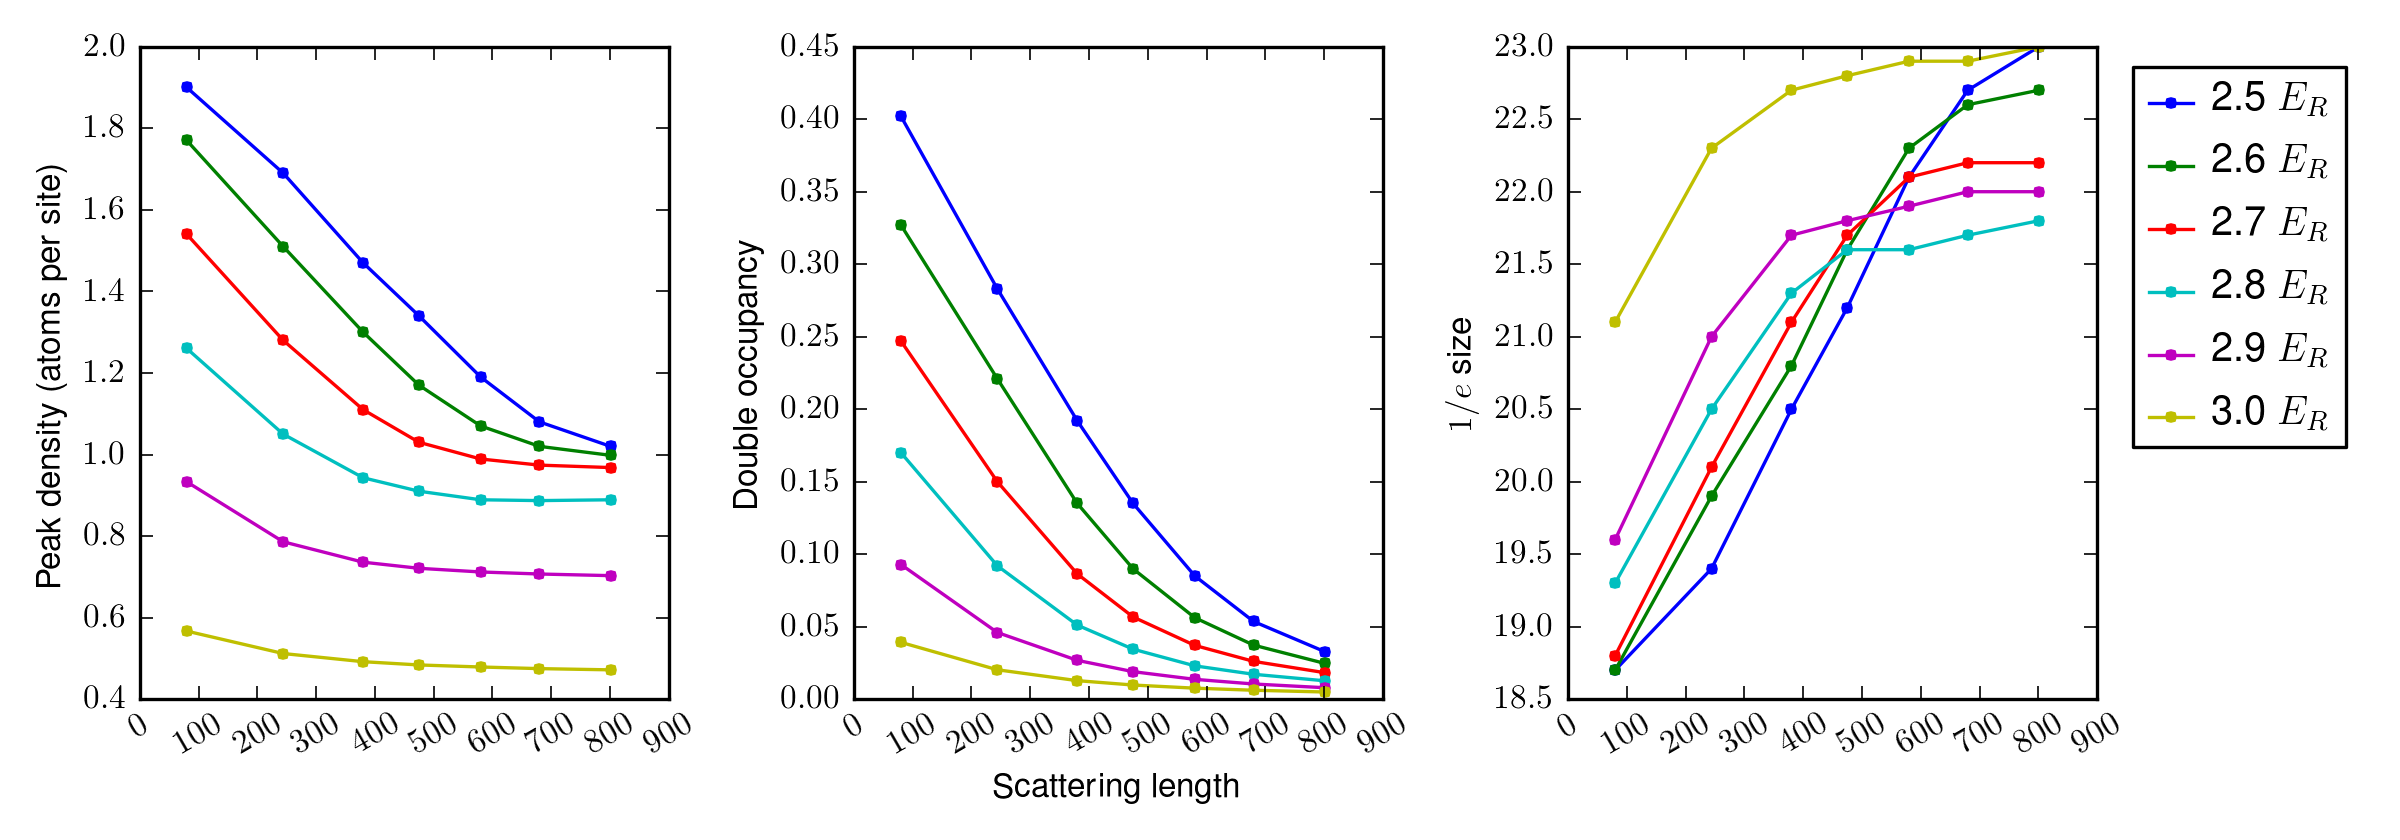
\includegraphics[width=\textwidth]{figures_140129/GR.png}
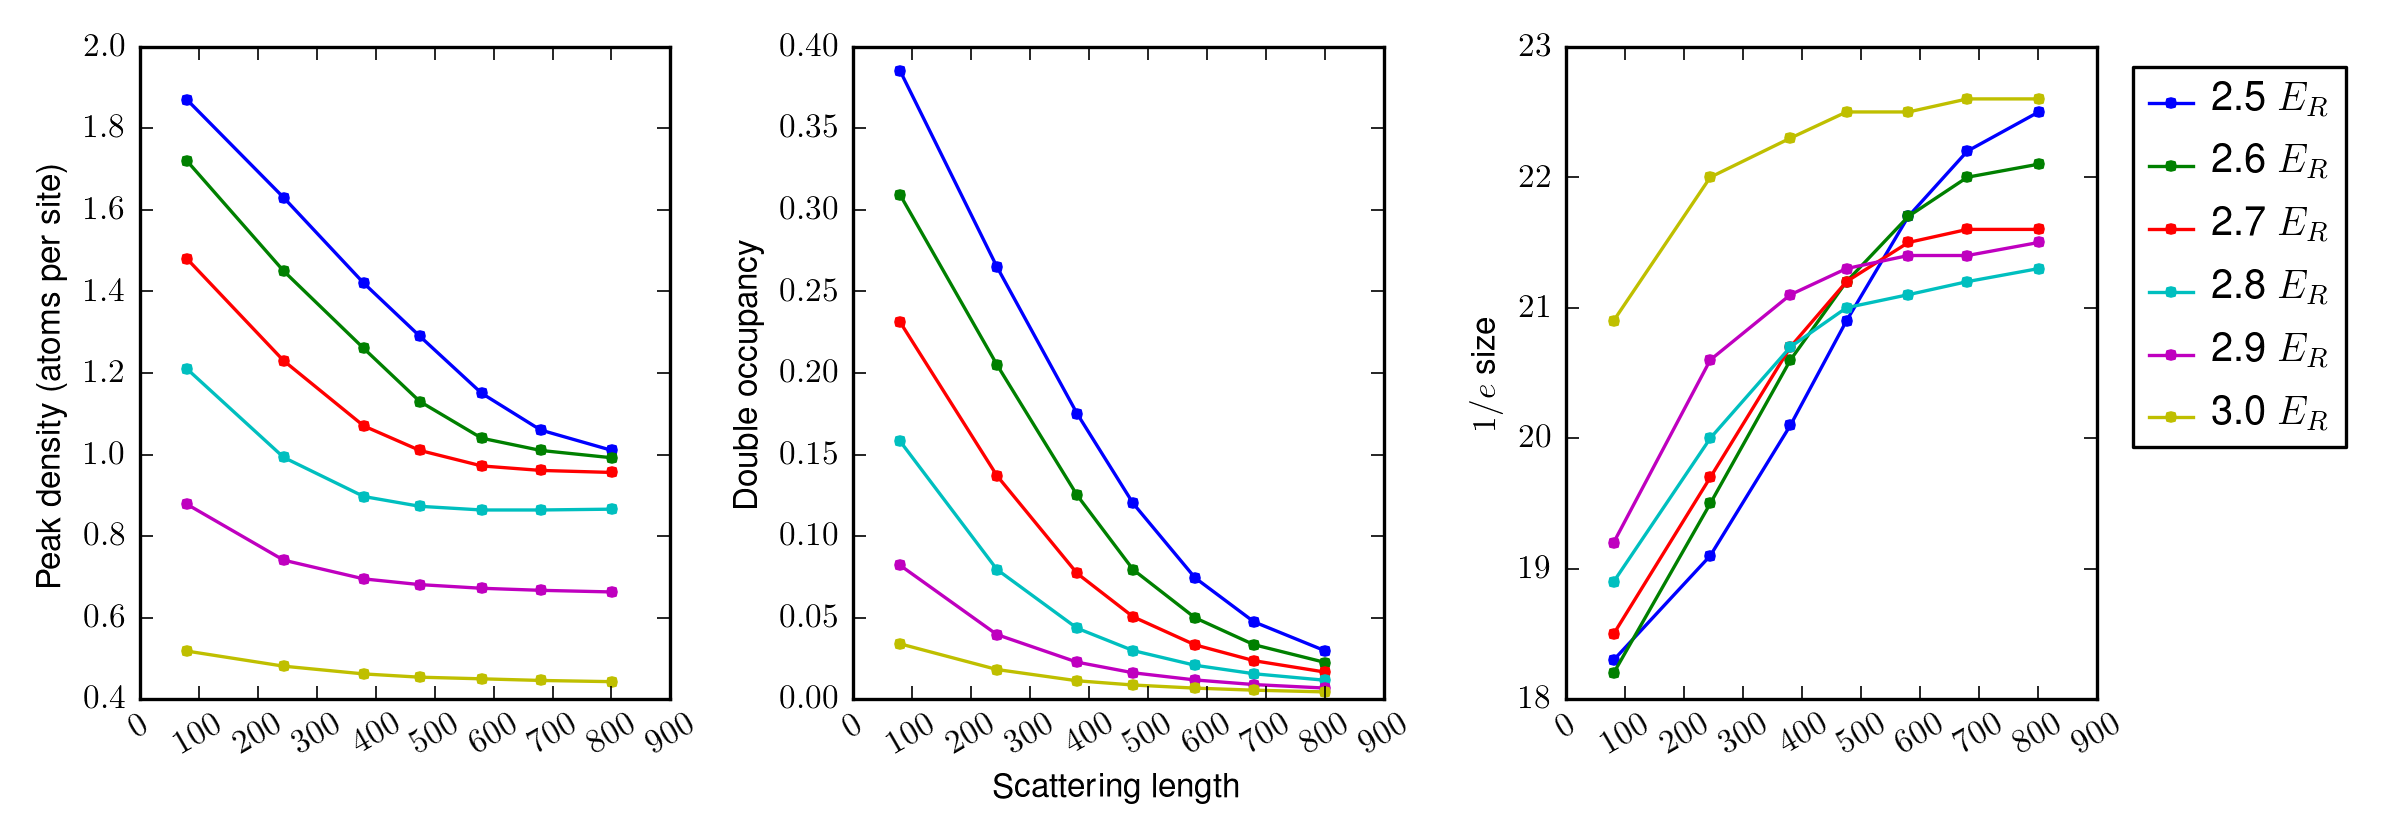
\includegraphics[width=\textwidth]{figures_140130/GR.png}
\caption[System parameters in the thermodynamic model]{\small 
System parameters as a function of scattering length for various values of the
green compensation.  The model used is the high temperature series expansion. }
\label{fig:thermo-green} 
\end{figure} 
The peak density and double occupancy depend sensitively on the green
compensation.  In order to calculate the density profiles that will be used to
estimate the effect of inhomogeneity on the spin structure factor we have to
pick a value for the green compensation.  The value that we use in the
experiment is 3\,$E_{R}$, but our observations of the peak density and the
double occupancy as a function of scattering length do not match the model at
3\,$E_{R}$ compensation.  Our measurement of the double occupancy in the
5.5\,$E_{R}$ lattice is shown in Fig.~\ref{fig:docc-5.5} and it resembles the
curve with a compensation of 2.7\,$E_{R}$ in the model.  
\begin{figure}
\centering 
%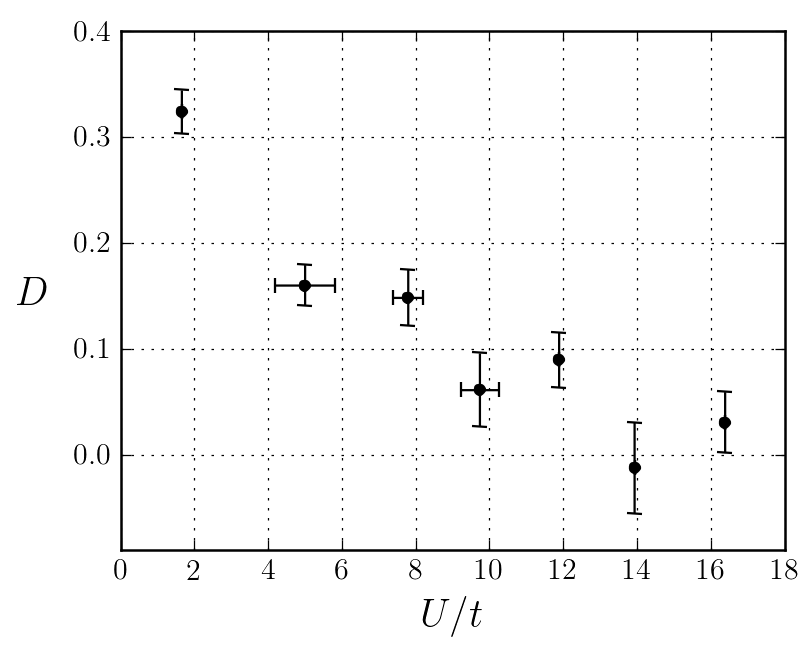
\includegraphics[width=0.4\textwidth]{figures_140129/docc_average.png}
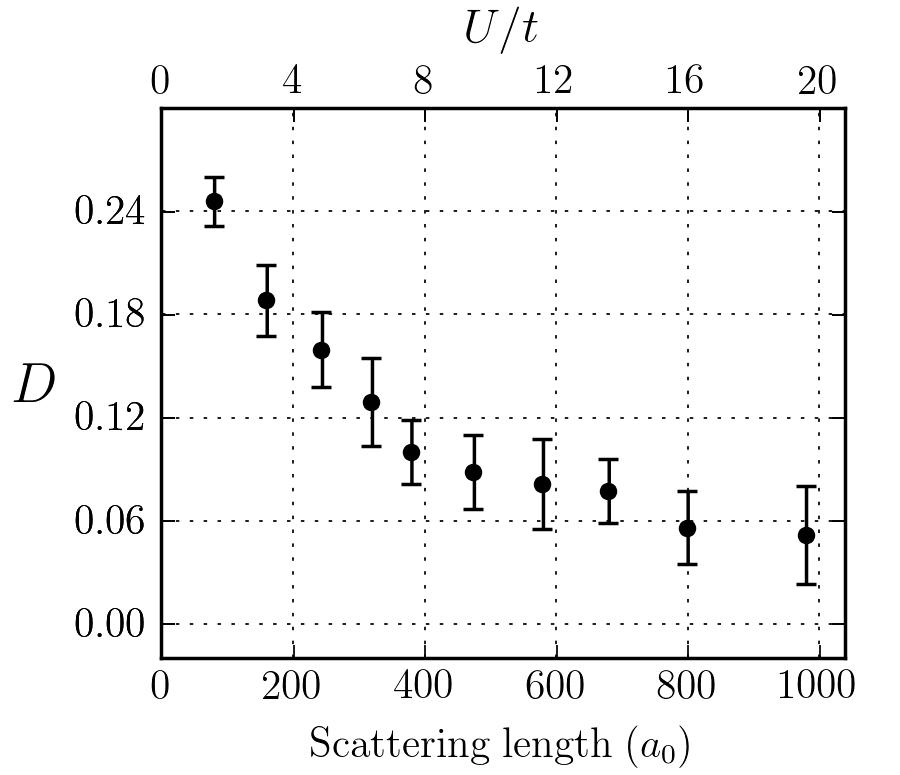
\includegraphics[width=0.4\textwidth]{figures_140130/insitu_D.png}
\caption[Double occupancy]{\small 
Double occupancy in the 5.5\,$E_{R}$ lattice. }
\label{fig:docc-5.5} 
\end{figure} 
 Our measurement of the density as a function of scattering length is shown in
Fig.~\ref{fig:dens-5.5} along with the measurement of the atom number. 
\begin{figure}
\centering
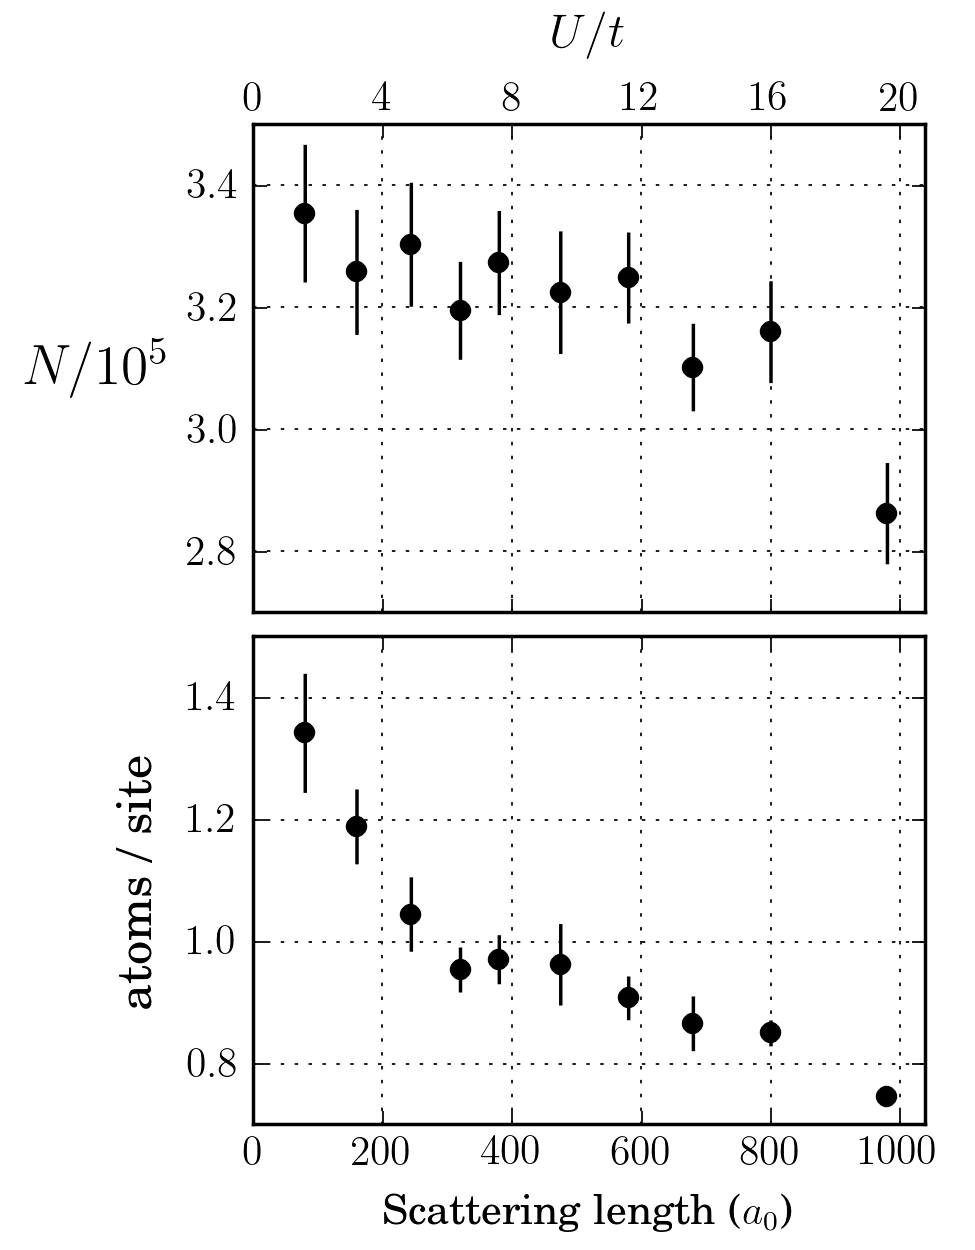
\includegraphics[width=0.4\textwidth]{figures_140130/insitu_density.png}
\caption[Peak density and atom number]{\small Peak density and atom number in
the 5.5\,$E_{R}$ lattice. The plateau in the density is characteristic of the
insulating state.  As the scattering length is increased three-body losses
become important as it is seen in both the atom number losses and decrease in
the peak density. }
\label{fig:dens-5.5} 
\end{figure}
Both the density and double occupancy measurements are consistent with a
compensation of 2.7\,$E_{R}$ in the model.   Discrepancies between our
measurements and the model is most likely due to calibration errors and our
inexact knowledge of the potential, however since the temperature used for the
model is $T/t = 1.8$ it is possible that the discrepancy is also  due to a
lower temperature in our system  than the one this model can handle.   In what
follows we will use 2.7\,$E_{R}$ in the model to stay  consistent with our
observations.  

With all the parameters that go into the model in hand, we can go ahead and
calculate density distributions.  We then split those density distributions
into bins with an equal number of atoms and calculate the filling $n$, and the
Hubbard parameters $U$ and $t$ for each bin.   An example of this calculation
for a scattering length of 580~$a_{0}$, which corresponds to $U/t$ at the
center equal to 11.9 is shown in Fig.~\ref{fig:bin-580a0}.
\begin{figure}
\centering
%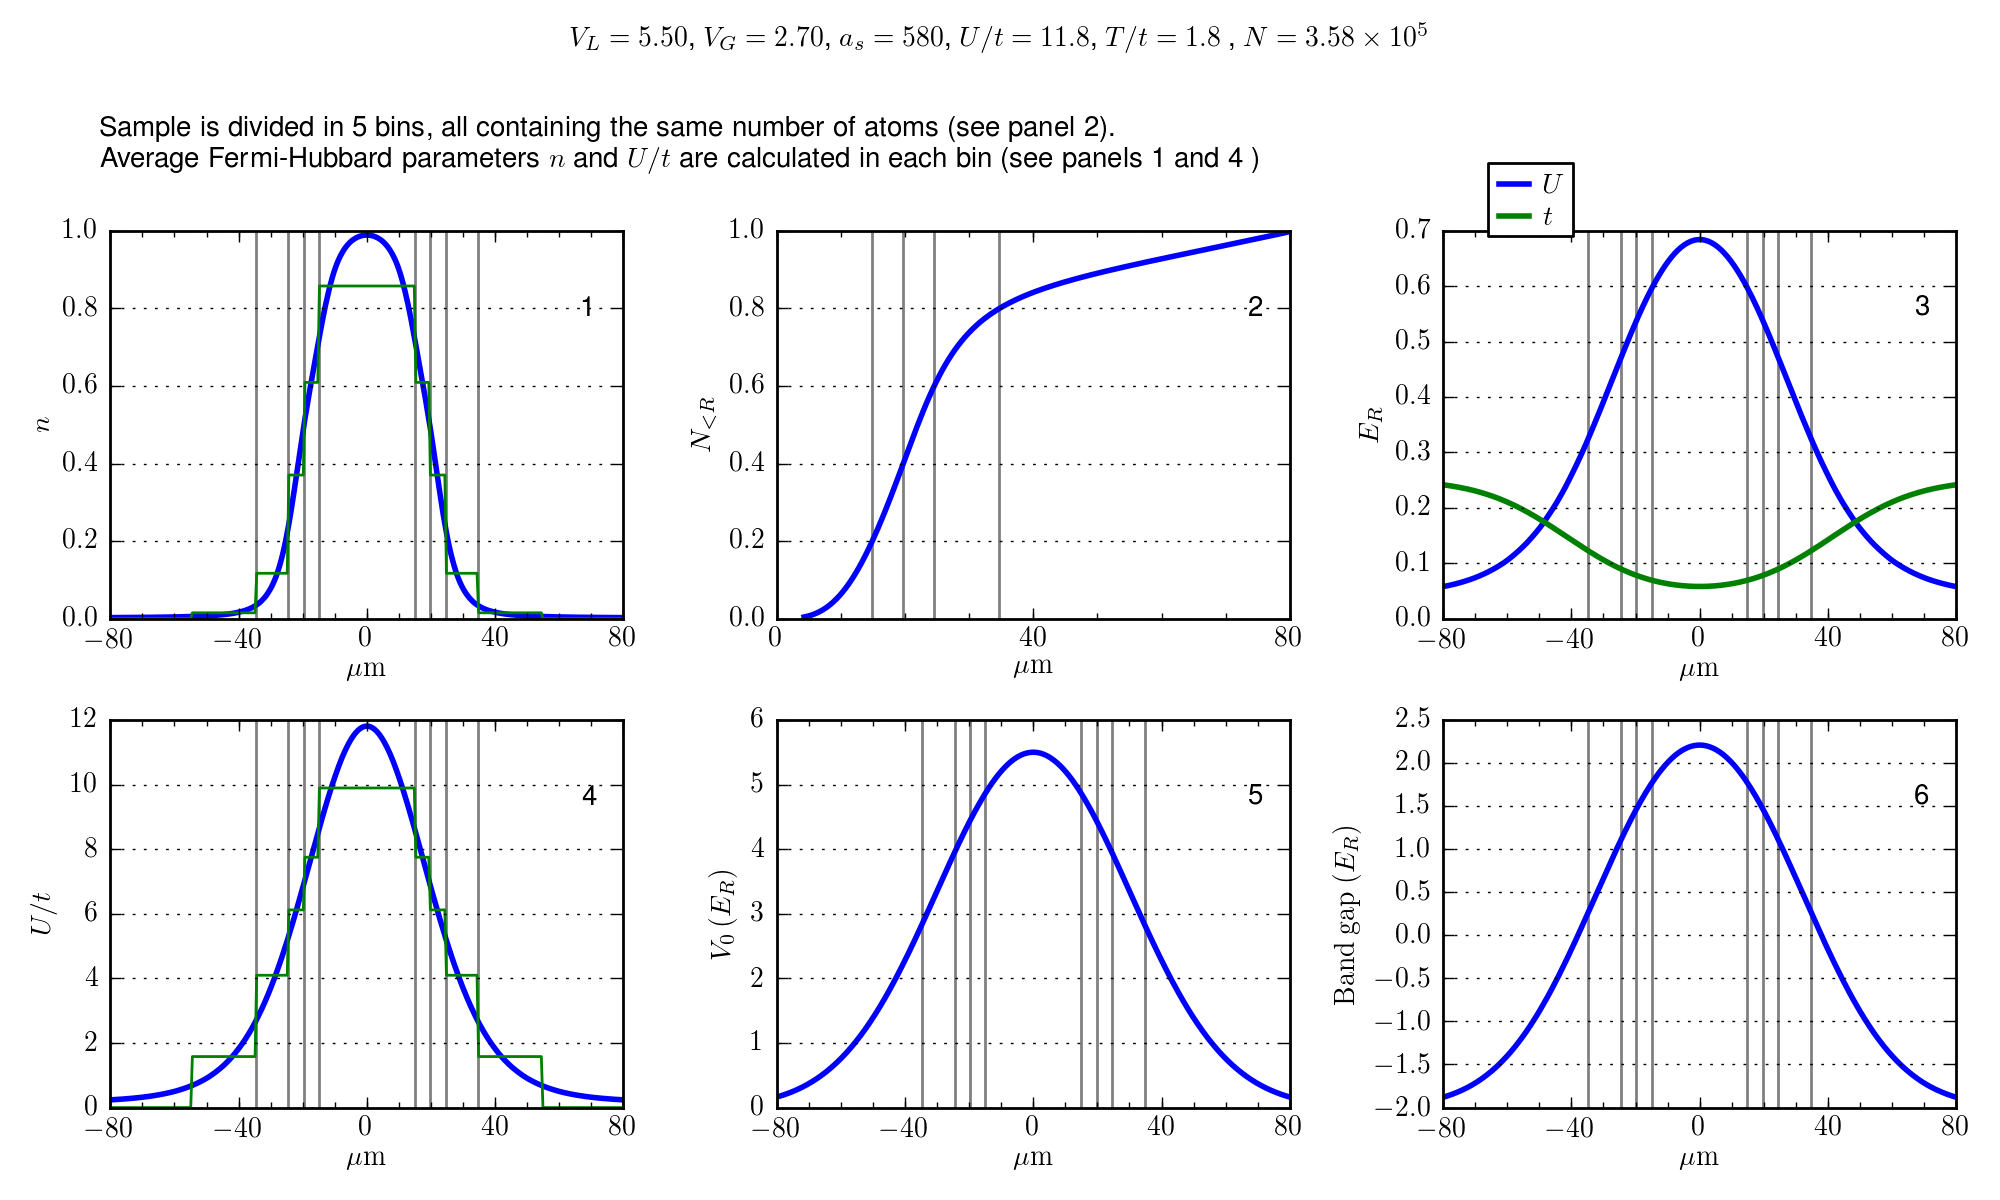
\includegraphics[width=\textwidth]{figures_140129/bin_5p5Er_2p7Gr580a0.png}
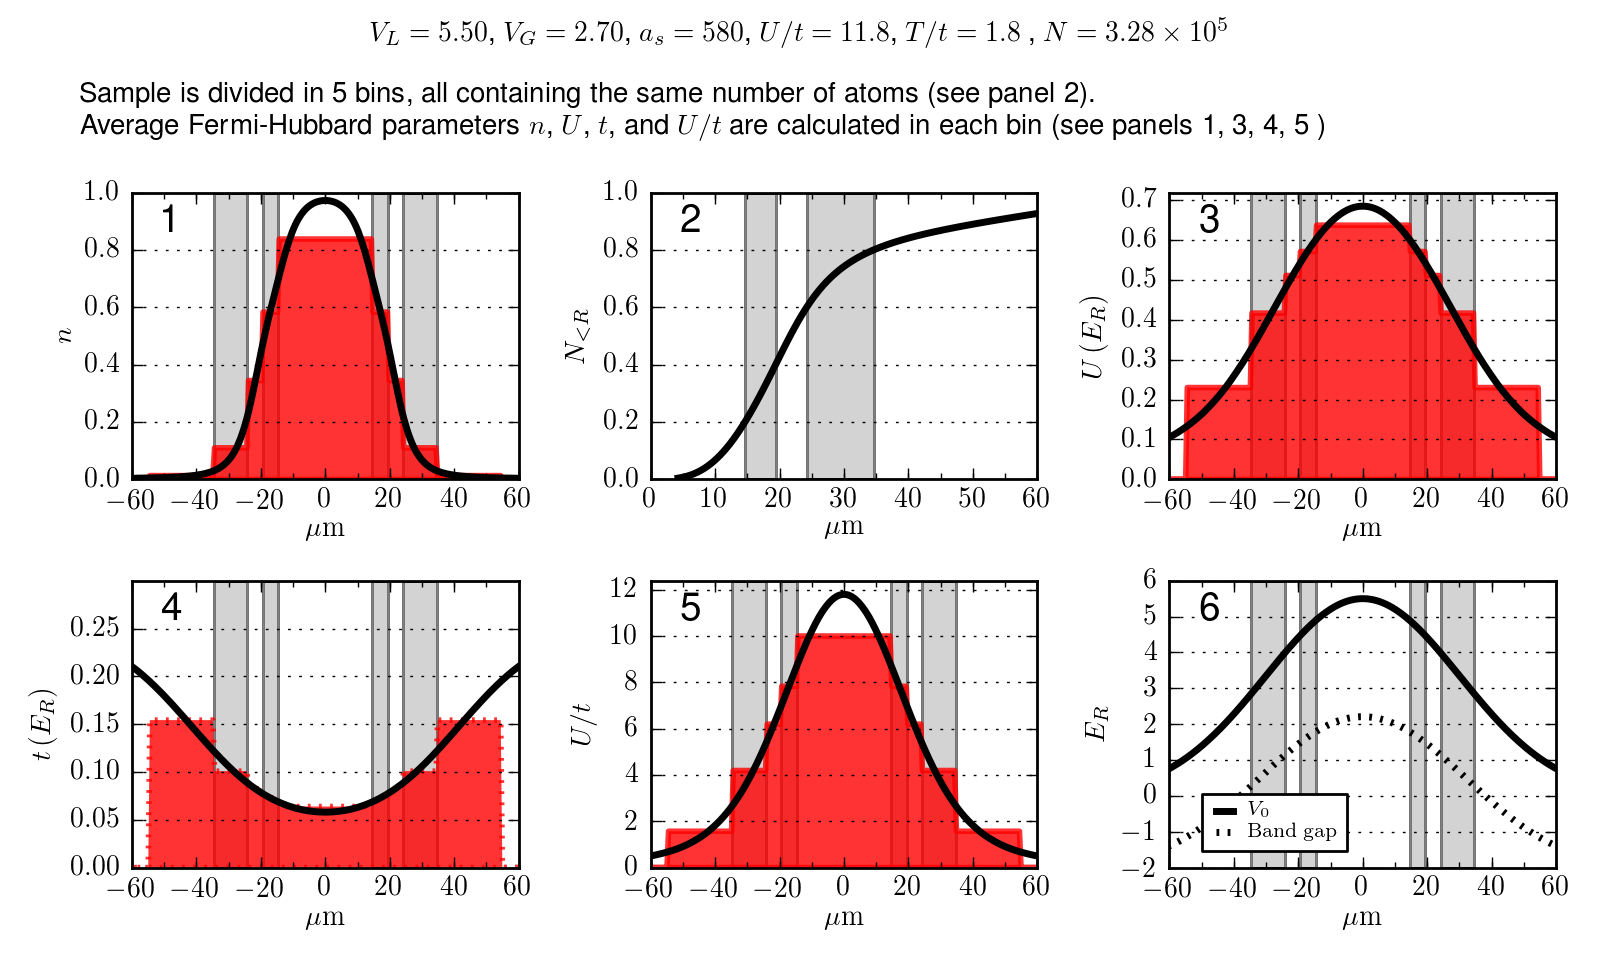
\includegraphics[width=\textwidth]{figures_140130/111_0580a0.png}
\caption[Binned density distribution]{\small Binned filling and Hubbard
parameters are shown in panels 1, 3, 4, and 5. The average value in each bin is
shown as the shaded red area. The cumulative number up to a certain radius is
shown in panel 2,  this illustrates how all the bins have the same number of
atoms.  The lattice depth and band gap as a function of radius are shown in
panel 6. }
\label{fig:bin-580a0} 
\end{figure} 

In the averaging of the bins to calculate the structure factor we will assume
that the entire system is isothermal at some temperature $T$,  this corresponds
to a reduced temperature $T/t$ at the center of the sample.  In a given bin,
$b$,  the reduced temperature (which will be relevant for the QMC in the bin)
is given by \[  \frac{T}{t_{b}} = \left( \frac{T}{t} \right) \frac{t}{t_{b}} \]
where $t$ is the tunneling at the center of the sample and $t_{b}$ is the
average tunneling in $b^{\mathrm{th}}$ bin.

Table~\ref{table:bin580} shows an example of the binning results for a value
of $U/t = 11.86$ at the center of the sample.
\begin{table}
\centering
\begin{minipage}[b][10em][b]{0.36\textwidth}
\begin{verbatim}
-------------------------------
At center:
  t = 0.058 Er
  U = 0.687 Er
U/t = 11.860 Er

At bins:
bin#     nb     t/tb      Ub/tb     
-------------------------------
000    0.84     0.91       9.97
001    0.58     0.79       7.82
002    0.34     0.70       6.19
003    0.11     0.57       4.13
004    0.01     0.38       1.49
\end{verbatim}
\end{minipage}
\caption[Binning for $U/t=11.86$]{Binning for $U/t=11.86$}
\label{table:bin580} 
\end{table}
The table shows first the values of the parameters at the center of the sample,
and then for each bin the columns show respectively $n_{b}$, $t/t_{b}$, and
$U_{b}/t_{b}$.   These three values are what is needed to perform the QMC
calculation in each bin.  

Below, in Table~\ref{table:binall}, we produce seven tables like
Table~\ref{table:bin580} for the seven different values of $U/t$ at the center
that correspond to our structure factor data in the $5.5\,E_{R}$ lattice.  We
add a column labeled $u$, which corresponds to the ratio of $U_{b}/t_{b}$ to
$U/t$ at the center.   
\begin{table}
\vspace{4em}
{ \scriptsize
\begin{minipage}[b][10em][b]{0.33\textwidth}
\begin{verbatim}
-------------------------------
At center:
  t = 0.058 Er
  U = 0.095 Er
U/t = 1.636 Er

At bins:
bin#    nb   t/tb   Ub/tb     u     
-------------------------------
000   1.18   0.93   1.42   0.87
001   0.79   0.83   1.17   0.71
002   0.45   0.74   0.95   0.58
003   0.14   0.62   0.67   0.41
004   0.02   0.41   0.27   0.17
\end{verbatim}
\end{minipage}
\begin{minipage}[b][10em][b]{0.33\textwidth}
\begin{verbatim}
-------------------------------
At center:
  t = 0.058 Er
  U = 0.288 Er
U/t = 4.976 Er

At bins:
bin#    nb   t/tb   Ub/tb     u     
-------------------------------
000   0.99   0.91   4.25   0.86
001   0.66   0.81   3.41   0.69
002   0.39   0.72   2.75   0.55
003   0.12   0.60   1.90   0.39
004   0.02   0.40   0.73   0.16
\end{verbatim}
\end{minipage}
\begin{minipage}[b][10em][b]{0.33\textwidth}
\begin{verbatim}
-------------------------------
At center:
  t = 0.058 Er
  U = 0.450 Er
U/t = 7.771 Er

At bins:
bin#    nb   t/tb   Ub/tb     u     
-------------------------------
000   0.89   0.91   6.54   0.84
001   0.61   0.80   5.19   0.67
002   0.37   0.71   4.17   0.54
003   0.12   0.59   2.83   0.37
004   0.01   0.39   1.05   0.14
\end{verbatim}
\end{minipage}

\vspace{8em}

\begin{minipage}[b][10em][b]{0.33\textwidth}
\begin{verbatim}
-------------------------------
At center:
  t = 0.058 Er
  U = 0.563 Er
U/t = 9.713 Er

At bins:
bin#    nb   t/tb   Ub/tb     u     
-------------------------------
000   0.85   0.91   8.17   0.84
001   0.60   0.80   6.48   0.67
002   0.36   0.71   5.14   0.53
003   0.11   0.58   3.42   0.36
004   0.01   0.38   1.27   0.14
\end{verbatim}
\end{minipage}
\begin{minipage}[b][10em][b]{0.33\textwidth}
\begin{verbatim}
-------------------------------
At center:
  t = 0.058 Er
  U = 0.687 Er
U/t = 11.860 Er

At bins:
bin#    nb   t/tb   Ub/tb     u     
-------------------------------
000   0.84   0.91   9.97   0.84
001   0.58   0.79   7.82   0.66
002   0.34   0.70   6.19   0.52
003   0.11   0.57   4.13   0.35
004   0.01   0.38   1.49   0.13
\end{verbatim}
\end{minipage}
\begin{minipage}[b][10em][b]{0.33\textwidth}
\begin{verbatim}
-------------------------------
At center:
  t = 0.058 Er
  U = 0.806 Er
U/t = 13.905 Er

At bins:
bin#    nb   t/tb   Ub/tb     u     
-------------------------------
000   0.83   0.91  11.69   0.84
001   0.58   0.79   9.17   0.66
002   0.35   0.70   7.25   0.52
003   0.11   0.57   4.84   0.35
004   0.01   0.38   1.75   0.13
\end{verbatim}
\end{minipage}

\vspace{8em}

\begin{minipage}[b][10em][b]{0.33\textwidth}
\begin{verbatim}
-------------------------------
At center:
  t = 0.058 Er
  U = 0.948 Er
U/t = 16.359 Er

At bins:
bin#    nb   t/tb   Ub/tb     u     
-------------------------------
000   0.83   0.91  13.78   0.84
001   0.57   0.79  10.80   0.66
002   0.33   0.70   8.43   0.52
003   0.10   0.57   5.51   0.34
004   0.01   0.37   1.98   0.13
\end{verbatim}
\end{minipage}
}
\caption[Binning for various values of $U/t$]{Binning for various values of $U/t$}
\label{table:binall} 
\end{table}

We point out that the $n$, $t/t_{b}$ and $u$ columns do not differ much across
the different values of $U/t$ at the center.   To simplify the matter, and
since this treatment is only a crude estimation we create a single table,
Table~\ref{table:binavg}, which averages the binnings for the seven values of
$U/t$ at the center.   In this way we obtain a binning with which we can
represent the inhomogeneity of our sample in a general case.  

\begin{table}
\centering
\begin{minipage}[b][10em][b]{0.36\textwidth}
\begin{verbatim}
--------------------------------
bin#      nb     t/tb         u
--------------------------------
000    0.92      0.91      0.85
001    0.63      0.80      0.67
002    0.37      0.71      0.54
003    0.12      0.59      0.37
004    0.01      0.39      0.14
\end{verbatim}
\end{minipage}
\caption[Binning for general case]{Binning for general case.   To estimate the
trap averaged structure factor at a temperature $T/t\equiv x$ and with an
interaction given by $U/t\equiv y$,  a QMC calculation will be performed for
each bin using filling $n_{b}$, temperature $x(t/t_{b})$ and interaction
strength $yu$.  }
\label{table:binavg} 
\end{table}


\subsection{Raw data for $S_{\pi}/S_{\theta}$ and $S_{\pi}$ }

Below we show the raw data for the best estimate of $S_{\pi}/S_{\theta}$ which uses the simultaneous measurement of both cameras with a calibrated normalization.  This is panel 3 on the figure with the data. 

\begin{verbatim}
----------------------
 U/t  Spi/Sth   error
----------------------
 1.6     1.21   0.065
 5.0     1.32   0.099
 7.8     1.34   0.098
 9.7     1.48   0.108
11.9     1.64   0.110
13.9     1.35   0.140
16.4     1.24   0.136
\end{verbatim}

\vspace{2em}

Below we show $S_{\bv{\pi}}$ determined from $S_{\bv{\pi}}/S_{\bv{\theta}}$ and $S_{\bv{\theta}}$, this is panel 5 on the figure with the data .

\begin{verbatim}
----------------------
 U/t     Spi   error
----------------------
 1.6   0.735   0.055
 5.0   0.923   0.078
 7.8   1.021   0.087
 9.7   1.141   0.099
11.9   1.199   0.099
13.9   1.168   0.138
16.4   1.031   0.123
\end{verbatim}

\vspace{2em}
\newpage

Below we show $S_{\bv{\pi}}$ determined using only the camera at $\bv{\pi}$, this is panel 2 on the figure with the data.   

\begin{verbatim}
----------------------
 U/t     Spi   error
----------------------
 1.6   0.639   0.049
 5.0   0.882   0.078
 7.8   0.963   0.094
 9.7   1.162   0.124
11.9   1.331   0.096
13.9   1.240   0.172
16.4   1.069   0.125
\end{verbatim}
 



\newpage 


%%%\subsection{Signal to noise considerations} 
%%%
%%%It seems obvious that one would want to operate in a regime where $\iisat \ll
%%%1$ and $e^{-2W} = 1$.   The maximum lattice depth that we can achieve is
%%%50$E_{R}$, so that sets the value of $e^{-2W}$.  The intensity that we use es
%%%conditioned by noise associated with the measurement of the intensity using a
%%%CCD.  
%%%
%%%We add up the counts on a set of pixels of the CCD as a measurement of the
%%%intensity.  The dark noise on the counts is $\delta D \approx 500$.  Using an
%%%intensity of $\iisat \approx 15$ we measure $\bar{I} \approx 3000$.  We define
%%%\begin{equation}
%%% \beta = \frac{ \bar{I} }{ \iisat } \approx  200 
%%%\end{equation}
%%%
%%%Using the abbreviation $I_{t}= \frac{I}{I_{\text{TOF}}}$, and the fact that our
%%%determination of $I$ and $I_{\text{TOF}}$ is dark noise dominated 
%%%\begin{equation}
%%% \delta I_{t}  =  (\bar{ I}_{\text{TOF} })^{-1} 
%%%        \sqrt{  \delta I^{2}  
%%%             +  I_{t}^{2}\left( \delta I_{\text{TOF}}\right)^{2} }
%%%    = (\bar{ I}_{\text{TOF} })^{-1} \delta D \sqrt{ 1 + I_{t}^{2}}
%%%    = \frac{ \delta D } { \beta ( \iisat ) }  \sqrt{ 1 + I_{t}^{2}}
%%%\end{equation}
%%%
%%%The relative uncertainty for the spin structure factor is 
%%%\begin{equation} 
%%%  \frac{ \delta S }{ S } = 
%%%  \frac{ \delta I_{t} }{ 
%%%  \frac
%%%        { e^{-2W}}  
%%%        {1  +   \frac{\iisat}{2\Delta^{2} } } 
%%% +  (I_{t} - 1)  } 
%%%  = 
%%%  \frac{ 1 }{ 
%%%  \frac
%%%        { e^{-2W}}  
%%%        {1  +   \frac{\iisat}{2\Delta^{2} } } 
%%% +  (I_{t} - 1)  } 
%%%\frac{ \delta D } { \beta ( \iisat ) }  \sqrt{ 1 + I_{t}^{2}}
%%%\end{equation}
%%%
%%%Say the value of $I_{t}$ we are going to measure is around 1.2,  then also using
%%%$e^{-2W}=0.81$, $\beta=200$, $\delta D=500$, $\Delta=6.5$ we get 
%%%\begin{equation} 
%%%  \frac{ \delta S }{ S } =  
%%%  \frac{ 1 }{ 
%%%  \frac
%%%        { e^{-2W}}  
%%%        {1  +   \frac{\iisat}{2\Delta^{2} } } 
%%% +  (I_{t} - 1)  } 
%%%\frac{ \delta D } { \beta ( \iisat ) }  \sqrt{ 1 + I_{t}^{2}}
%%%\end{equation}
%%%
%%%%%%%%\subsection{Walk through Ted's derivation to find missing terms}\label{sec:Ted}
%%%%%%%%
%%%%%%%%We start with Ted's formula for the differential cross section
%%%%%%%%\begin{equation}
%%%%%%%%\begin{split}
%%%%%%%%\dsig{} =& \frac{9}{4k^{2}}
%%%%%%%%              \sum_{\lambda_{f}} | (\bv{e}_{\bv{k}_{f} \lambda_{f}}^{*} \cdot \bv{e}_{m} )
%%%%%%%%                                   (\bv{e}_{m}^{*} \cdot \bv{e}_{\bv{k}_{i} \lambda_{i}}^{*} )
%%%%%%%%                                 |^{2} \\
%%%%%%%%          & \times \sum_{ \sigma,\sigma', j, j' } [ \langle \hat{n}_{j\sigma}\hat{n}_{j'\sigma'}
%%%%%%%%              e^{ i \bv{K} \cdot ( \hat{\bv{r}}_{j} - \hat{\bv{r}}_{j'} ) } \rangle
%%%%%%%%              \bar{f}_{\sigma} {\bar{f}_{\sigma'}}^{*} ]
%%%%%%%%\end{split}
%%%%%%%%\end{equation}
%%%%%%%%and we abbreviate the sum over final polarizations as
%%%%%%%%\begin{equation}
%%%%%%%% \Lambda = \sum_{\lambda_{f}} | (\bv{e}_{\bv{k}_{f} \lambda_{f}}^{*} \cdot \bv{e}_{m} )
%%%%%%%%                                   (\bv{e}_{m}^{*} \cdot \bv{e}_{\bv{k}_{i} \lambda_{i}}^{*} )
%%%%%%%%                                 |^{2}
%%%%%%%%\end{equation}
%%%%%%%%to obtain
%%%%%%%%
%%%%%%%%\begin{equation}
%%%%%%%%\begin{split}
%%%%%%%%\dsig{} =& \frac{9\Lambda}{4k^{2}}
%%%%%%%%               \sum_{ \sigma,\sigma', j, j' } [ \langle \hat{n}_{j\sigma}\hat{n}_{j'\sigma'}
%%%%%%%%              e^{ i \bv{K} \cdot ( \hat{\bv{r}}_{j} - \hat{\bv{r}}_{j'} ) } \rangle
%%%%%%%%              \bar{f}_{\sigma} {\bar{f}_{\sigma'}}^{*} ] \\
%%%%%%%%\end{split}
%%%%%%%%\end{equation}
%%%%%%%%
%%%%%%%%
%%%%%%%%We will begin by disecting the sum that appears in the elastic cross section. The thermal average factorizes and
%%%%%%%%\begin{equation}
%%%%%%%%\begin{split}
%%%%%%%%\langle \hat{n}_{j\sigma}\hat{n}_{j'\sigma'} \rangle = &\, \langle (\frac{1}{2} + \sigma\hat{S}_{zj} )( \frac{1}{2} + \sigma'\hat{S}_{j'} ) \rangle \\
%%%%%%%%       = &\, \frac{1}{4} + \frac{1}{2} \langle \sigma \hat{S}_{zj} \rangle +
%%%%%%%%\frac{1}{2} \langle \sigma'\hat{S}_{zj'} \rangle + \langle \sigma\sigma'\hat{S}_{zj}\hat{S}_{zj'}
%%%%%%%%\rangle \\
%%%%%%%%\end{split}
%%%%%%%%\end{equation}
%%%%%%%%For this last step
%%%%%%%%\begin{center}
%%%%%%%%  \begin{tabular}{ c }
%%%%%%%%    $\hat{n}_{i\uparrow} + \hat{n}_{i\downarrow} = 1$ \\
%%%%%%%%    $\sigma = \pm 1$ \\
%%%%%%%%    $\hat{S}_{zi} = \frac{1}{2}( \hat{n}_{i\uparrow} - \hat{n}_{i\downarrow} )$
%%%%%%%%  \end{tabular}
%%%%%%%%\end{center}
%%%%%%%%We can manually perform the sums over $\sigma\sigma'$ for each of this four terms and define $\alpha$, $\beta$, and $\kappa$,
%%%%%%%%\begin{equation}
%%%%%%%%\begin{split}
%%%%%%%%\frac{1}{4} \sum_{\sigma\sigma'} \bar{f}_{\sigma} \bar{f}_{\sigma'}^{*} = &\,
%%%%%%%%            \frac{1}{4}(\bar{f}_{\uparrow} + \bar{f}_{\downarrow})( \bar{f}_{\uparrow}^{*} + \bar{f}_{\downarrow}^{*} ) \\
%%%%%%%%       =&\, \frac{1}{4} | \bar{f}_{\uparrow} + \bar{f}_{\downarrow} | ^{2} \equiv \alpha
%%%%%%%%\end{split}
%%%%%%%%\end{equation}
%%%%%%%%
%%%%%%%%\begin{equation}
%%%%%%%%\begin{split}
%%%%%%%%\frac{1}{2} \sum_{\sigma\sigma'} \sigma'\bar{f}_{\sigma} \bar{f}_{\sigma'}^{*} = &\,
%%%%%%%%  \frac{1}{2} (
%%%%%%%%            - \bar{f}_{\downarrow}\bar{f}_{\downarrow}^{*}
%%%%%%%%            + \bar{f}_{\downarrow}\bar{f}_{\uparrow}^{*}
%%%%%%%%            - \bar{f}_{\uparrow}\bar{f}_{\downarrow}^{*}
%%%%%%%%            + \bar{f}_{\uparrow}\bar{f}_{\uparrow}^{*} ) \equiv \kappa
%%%%%%%%\end{split}
%%%%%%%%\end{equation}
%%%%%%%%
%%%%%%%%\begin{equation}
%%%%%%%%\begin{split}
%%%%%%%%\frac{1}{2} \sum_{\sigma\sigma'} \sigma \bar{f}_{\sigma} \bar{f}_{\sigma'}^{*} = &\,
%%%%%%%%  \frac{1}{2} (
%%%%%%%%            - \bar{f}_{\downarrow}\bar{f}_{\downarrow}^{*}
%%%%%%%%            - \bar{f}_{\downarrow}\bar{f}_{\uparrow}^{*}
%%%%%%%%            + \bar{f}_{\uparrow}\bar{f}_{\downarrow}^{*}
%%%%%%%%            + \bar{f}_{\uparrow}\bar{f}_{\uparrow}^{*} ) \equiv \kappa^{*}
%%%%%%%%\end{split}
%%%%%%%%\end{equation}
%%%%%%%%
%%%%%%%%\begin{equation}
%%%%%%%%\begin{split}
%%%%%%%%\sum_{\sigma\sigma'} \sigma\sigma' \bar{f}_{\sigma} \bar{f}_{\sigma'}^{*} = &\,
%%%%%%%%            (\bar{f}_{\uparrow} + \bar{f}_{\downarrow})( \bar{f}_{\uparrow}^{*} + \bar{f}_{\downarrow}^{*} ) \\
%%%%%%%%       =&\, | \bar{f}_{\uparrow} - \bar{f}_{\downarrow} | ^{2} \equiv \beta
%%%%%%%%\end{split}
%%%%%%%%\end{equation}
%%%%%%%%
%%%%%%%%The elastic cross section is then
%%%%%%%%\begin{equation}
%%%%%%%%\begin{split}
%%%%%%%%\dsig{E} =& \frac{9\Lambda}{4k^{2}}
%%%%%%%%               \sum_{ j j' } \langle
%%%%%%%%              e^{ i \bv{K} \cdot ( \hat{\bv{r}}_{j} - \hat{\bv{r}}_{j'} ) } \rangle
%%%%%%%%             \left( \alpha + \langle \hat{S}_{zj}\rangle \kappa + \langle \hat{S}_{zj'} \rangle \kappa^{*}
%%%%%%%%                     + \langle \hat{S}_{zj} \hat{S}_{zj'} \rangle \beta \right)
%%%%%%%%\end{split}
%%%%%%%%\end{equation}
%%%%%%%%
%%%%%%%%In the Bragg scattering paper by Ted, the two central terms are ignored, but there is no mention of why they are ignored.  As we saw above they also appear in the treatement of scattering that we have undertaken here.  
%%%%%%%%
%%%
%%%\section{Numerical evaluation of the scattered intensity}
%%%
%%%
%%%For the numerical calculation we start from Eq.~(\ref{eq:finalIdetector}) and replace the sum over $m<n$ with an unrestricted sum over $m,n$.  This removes the real part, and we have to subtract again some $m=n$ terms, the result is 
%%%\begin{multline}
%%% I  =
%%% \left( 
%%% \frac{\hbar c k \Gamma}{r_{D}^{2}}  
%%%     \frac{9}{24\pi} \Lambda 
%%%  \right) \times \\
%%%  \frac{ e^{-2W} }{ 4 (\iisat)} \sum_{mn} 
%%%    \frac{ s_{m} s_{n} } { ( 1+s_{m} )( 1+s_{n} ) }
%%%               e^{ i \bv{Q}( \bv{R}_{m} - \bv{R}_{n} ) }
%%%    \left(
%%%        4 \Delta_{m} \Delta_{n}
%%%      + 2 i \Delta_{n} 
%%%      - 2 i \Delta_{m}
%%%      + 1
%%%    \right)  
%%%  + \sum_{n}  \frac{1}{2}
%%%    \frac{ s_{n} } { 1 + s_{n} } \left( 1 - \frac{e^{-2W}}{1+s_{n}} \right)
%%%\end{multline}
%%%We will split this up as 
%%%\begin{multline}
%%% I  =
%%% \left( 
%%% \frac{\hbar c k \Gamma}{r_{D}^{2}}  
%%%     \frac{9}{24\pi} \Lambda 
%%%  \right) \times \\
%%%  \left[
%%%  \frac{ e^{-2W} }{ 4 (\iisat)}
%%%  \left( 
%%%    2 \sum_{m}  
%%%    \frac{ s_{m} }
%%%         {  1 + s_{m} } \Delta_{m} e^{i\bv{Q}\cdot\bv{R}_{m} }
%%%    2 \sum_{n} 
%%%    \frac{ s_{n} }
%%%         {  1 + s_{n} } \Delta_{n} e^{-i\bv{Q}\cdot\bv{R}_{n} }  \right. \right.\\
%%%    + 2i\sum_{m}  
%%%    \frac{ s_{m} }
%%%         {  1 + s_{m} } e^{i\bv{Q}\cdot\bv{R}_{m} }
%%%    \sum_{n} 
%%%    \frac{ s_{n} }
%%%         {  1 + s_{n} } \Delta_{n} e^{-i\bv{Q}\cdot\bv{R}_{n} }   \\
%%%    - 2i\sum_{m}  
%%%    \frac{ s_{m} }
%%%         {  1 + s_{m} } \Delta_{m} e^{i\bv{Q}\cdot\bv{R}_{m} }
%%%    \sum_{n} 
%%%    \frac{ s_{n} }
%%%         {  1 + s_{n} } e^{-i\bv{Q}\cdot\bv{R}_{n} }   \\
%%%    \left.
%%%    +\sum_{m}  
%%%    \frac{ s_{m} }
%%%         {  1 + s_{m} } e^{i\bv{Q}\cdot\bv{R}_{m} }
%%%    \sum_{n} 
%%%    \frac{ s_{n} }
%%%         {  1 + s_{n} } e^{-i\bv{Q}\cdot\bv{R}_{n} }  \right) \\
%%%   \left.
%%%  + \sum_{n}  \frac{1}{2}
%%%    \frac{ s_{n} } { 1 + s_{n} } \left( 1 - \frac{e^{-2W}}{1+s_{n}} \right) \right]
%%%\end{multline}
%%%The following sums appear and we define some shorthand notation for them
%%%\begin{align} 
%%%     \Phi \equiv & 
%%%     \sum_{m}  
%%%    \frac{ s_{m} }
%%%         {  1 + s_{m} } \Delta_{m} e^{i\bv{Q}\cdot\bv{R}_{m} } \\
%%%     \Upsilon \equiv &
%%%     \sum_{m}  
%%%    \frac{ s_{m} }
%%%         {  1 + s_{m} } e^{i\bv{Q}\cdot\bv{R}_{m} } \\
%%%     \kappa \equiv & 
%%%     \sum_{n}  
%%%     \frac{ s_{n} } { 1 + s_{n} }  \\
%%%     \xi \equiv & 
%%%     \sum_{n}  
%%%     \frac{ s_{n} } { (1 + s_{n})^{2}}  \\
%%%\end{align}
%%%We can then write the intensity as 
%%%\begin{equation}
%%%\begin{split}
%%% I  = &
%%% \left( 
%%% \frac{\hbar c k \Gamma}{r_{D}^{2}}  
%%%     \frac{9}{24\pi} \Lambda 
%%%  \right)
%%%  \left[
%%%  \frac{ e^{-2W} }{ 4 (\iisat)}
%%%  \left( 
%%%    4 \Phi \Phi^{*}
%%%    + 2i \Upsilon \Phi^{*} 
%%%    - 2i \Phi \Upsilon^{*}
%%%    + \Upsilon \Upsilon^{*}  
%%%          \right)
%%%  + \frac{1}{2}\kappa - \frac{ e^{-2W}}{2} \xi
%%%\right] \\ 
%%%\end{split}
%%%\end{equation}
%%%For the numerical evaluation we will use $\frac{\hbar c k \Gamma}{r_{D}^{2}}  
%%%     \frac{9}{48\pi}$  as a unit for the intensity, so we can finally simplify the expression to
%%%\begin{equation}
%%%\begin{split}
%%%  I  = &
%%% \Lambda 
%%%  \left[
%%%  \kappa + 
%%%  e^{-2W} \left(  
%%%  \frac{ | \Upsilon - 2 i \Phi |^{2} }{  2 (\iisat)}
%%%   - \xi \right)
%%%  \right] \\ 
%%%\end{split}
%%%\end{equation}
%%%We recall that 
%%%\begin{equation}
%%% \Lambda = 
%%%  \sum_{\bv{\varepsilon}' }
%%%        | (\bv{\varepsilon}_{+}\cdot \bv{\varepsilon}' )
%%%                        (\bv{\varepsilon}\cdot \bv{\varepsilon}_{-} ) |^{2} 
%%%\end{equation} 
%%%
%%%\subsection{Evaluation in a lattice with AFM core and random shell}
%%%
%%%For the numerical evaluation of the scattered intensity we will consider a
%%%lattice with $L\times L\times L$ sites in which there is a core of size
%%%$L_{\mathrm{AFM}} \times L_{\mathrm{AFM}} \times L_{\mathrm{AFM}}$ in which the
%%%atoms have antiferromagnetically ordered spins.   The distribution of the spins
%%%outside the core is random, but the spin imbalance is constrained to be zero,
%%%so there is an equal number of atoms in state $|1\rangle$ and state
%%%$|2\rangle $  occupying the $L^{3}$ sites in the lattice.
%%%
%%%\subsubsection{Available values of momentum transfer $\bv{Q}$}
%%%
%%%In our experiment we sample four different values of the momentum
%%%transfer vector $\bv{Q}$ by sending the probe beam in from different
%%%viewports in our vacuum chamber.   A schematic of this is shown in Fig.~\ref{fig:bragg_scattering_setup}. 
%%%\begin{figure}
%%%\centering 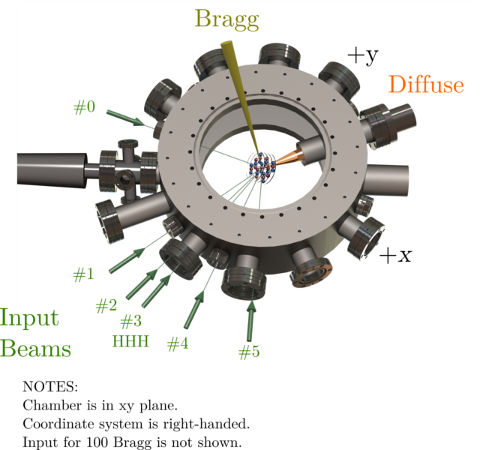
\includegraphics[width=0.75\textwidth]{figures/bragg_setup_illustration_320px.png}
%%%\caption[Bragg scattering setup]{\small Figure shows the different input directions that allow us to measure the spin structure factor at various values of the momentum transfer $\bv{Q}$.  }
%%%\label{fig:bragg_scattering_setup}
%%%\end{figure}
%%%
%%%\subsubsection{Debye-Waller factor} 
%%%
%%%We will start by showing plots of the Debye-Waller factor as a function of time-of-flight and lattice depth for some of the momentum transfer values.  Plots are as a function of lattice depth (Fig.~\ref{fig:debye-waller_HHH_v0}) and also time-of-flight for a 20 recoil lattice (Fig.~\ref{fig:debye-waller_HHH_tof}).
%%%\begin{figure}
%%%\centering 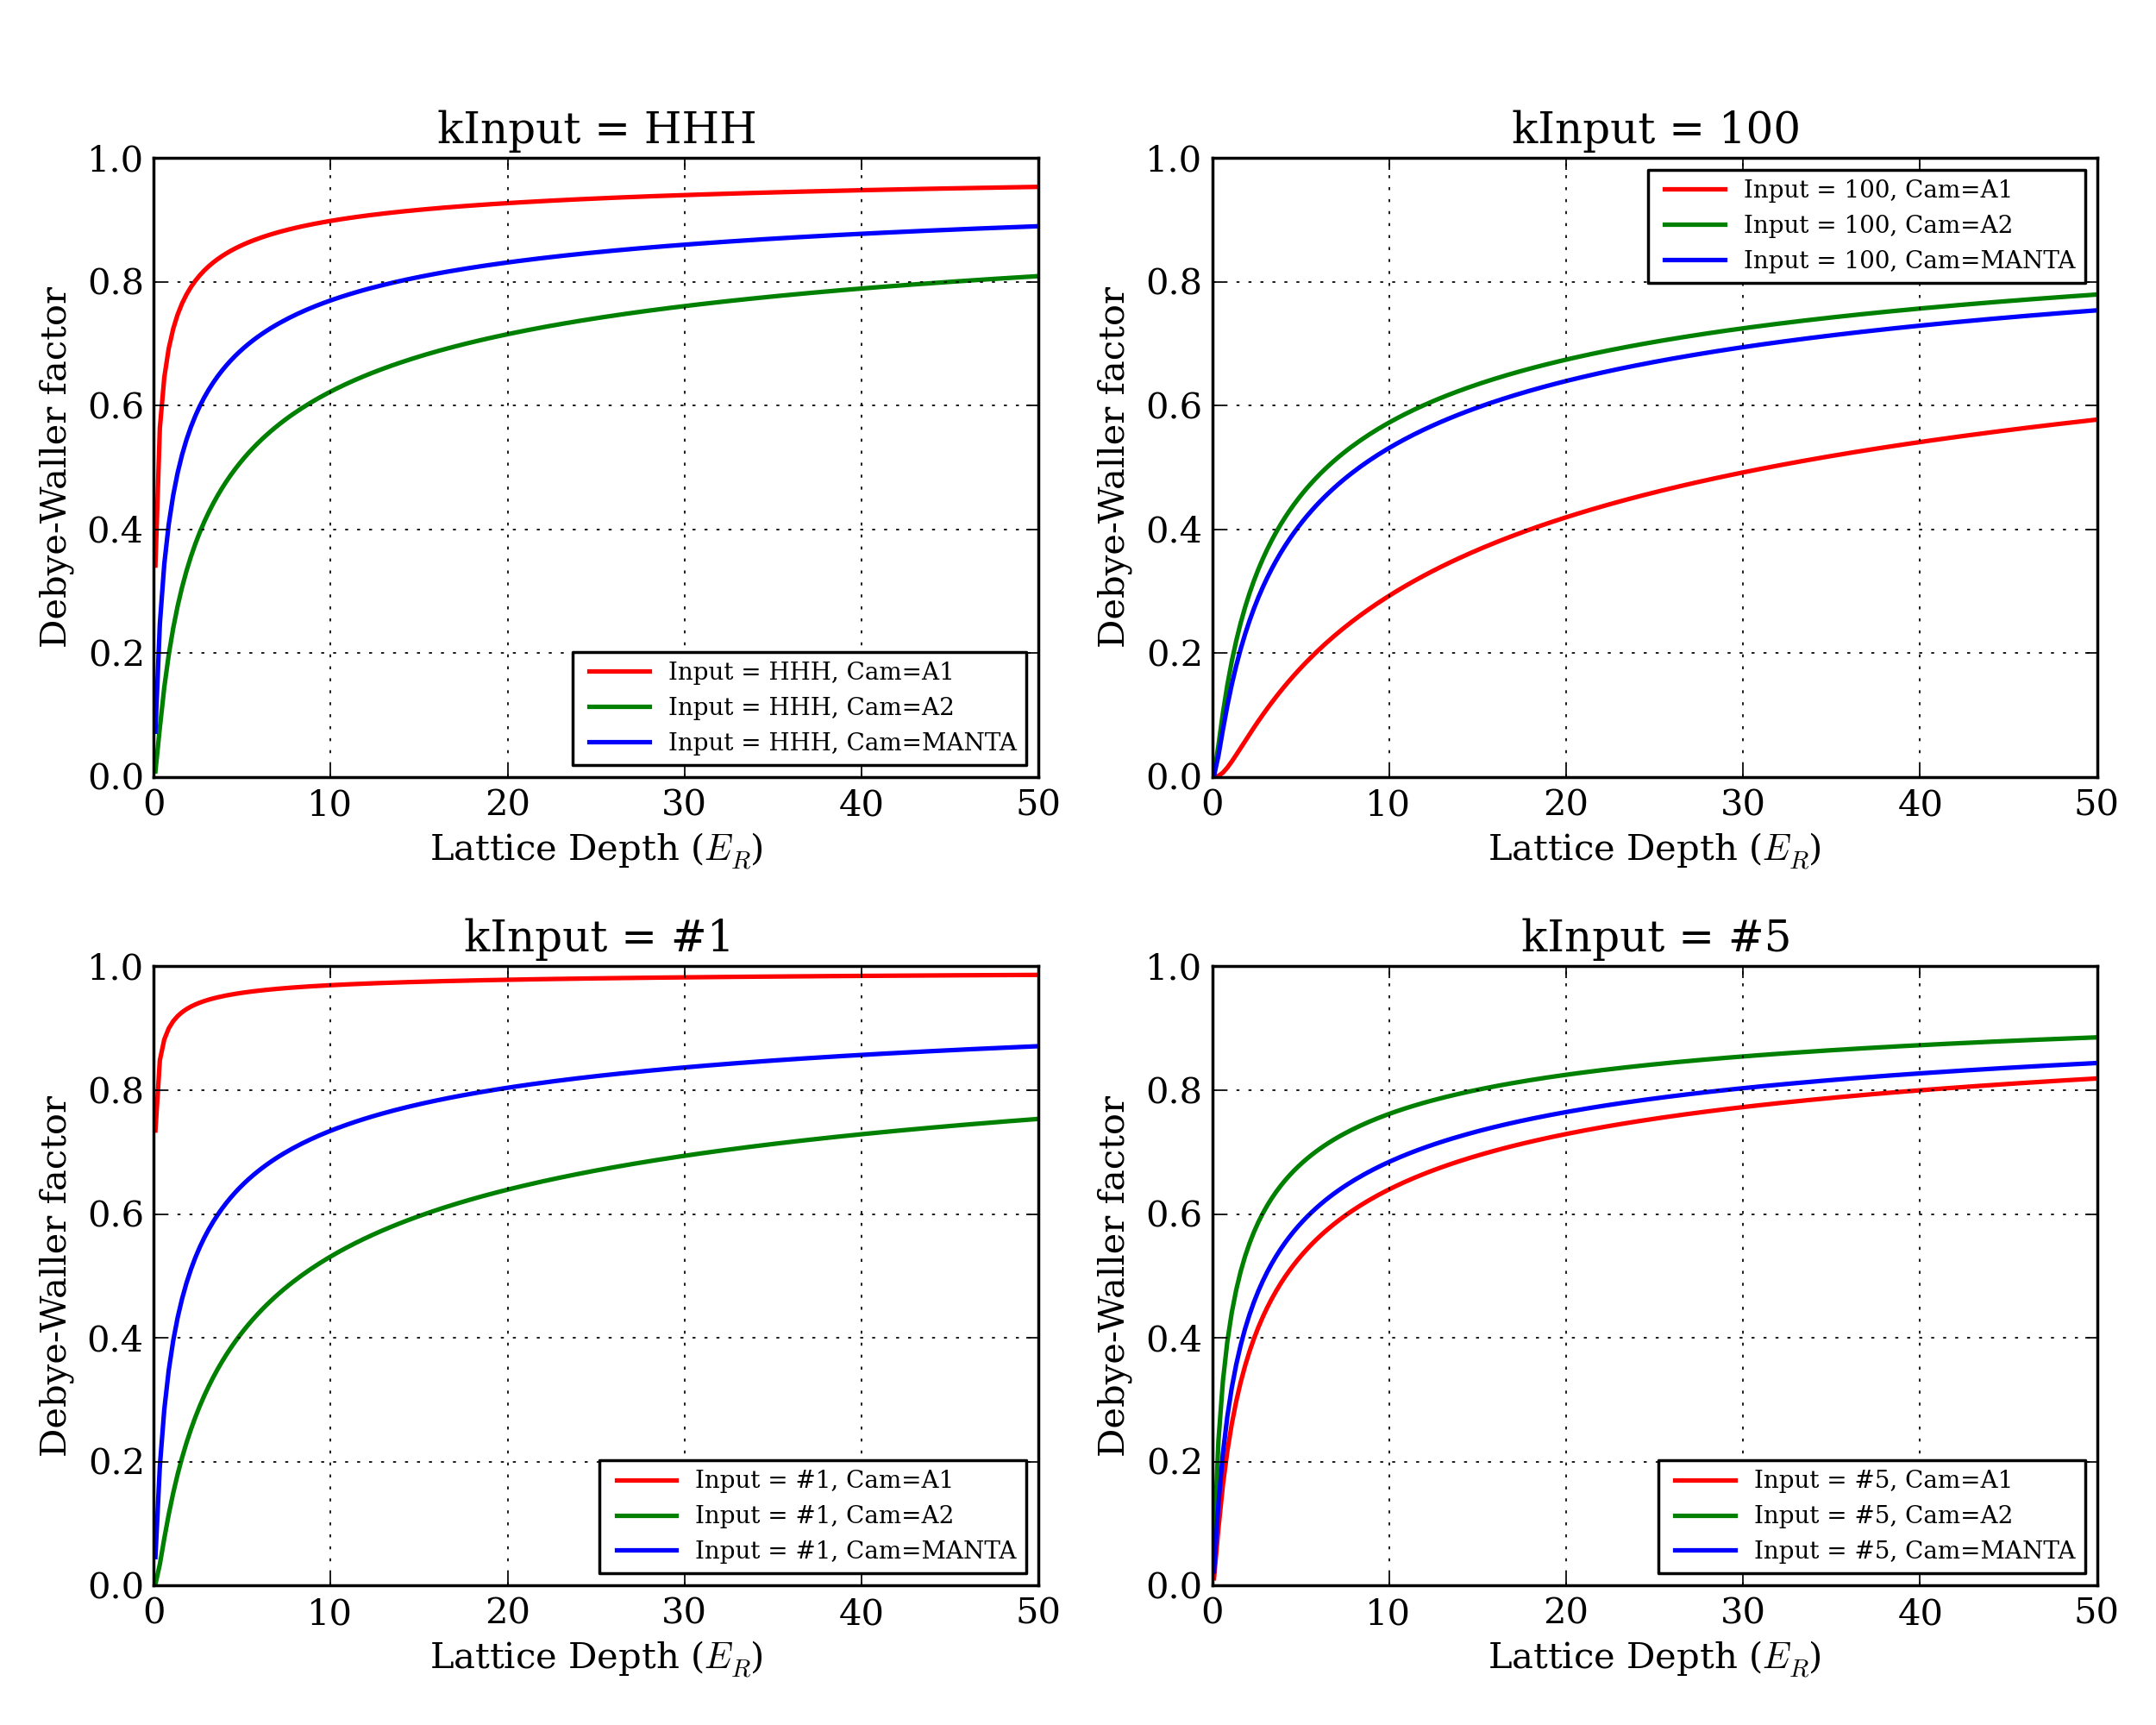
\includegraphics[width=\textwidth]{../debye-waller_HHH/DWv0_plot.png}
%%%\caption[Debye-Waller vs. Lattice depth]{\small Figure shows the Debye-Waller factor as a function of lattice depth for different momentum transfers.}
%%%\label{fig:debye-waller_HHH_v0}
%%%\end{figure}
%%%\begin{figure}
%%%\centering 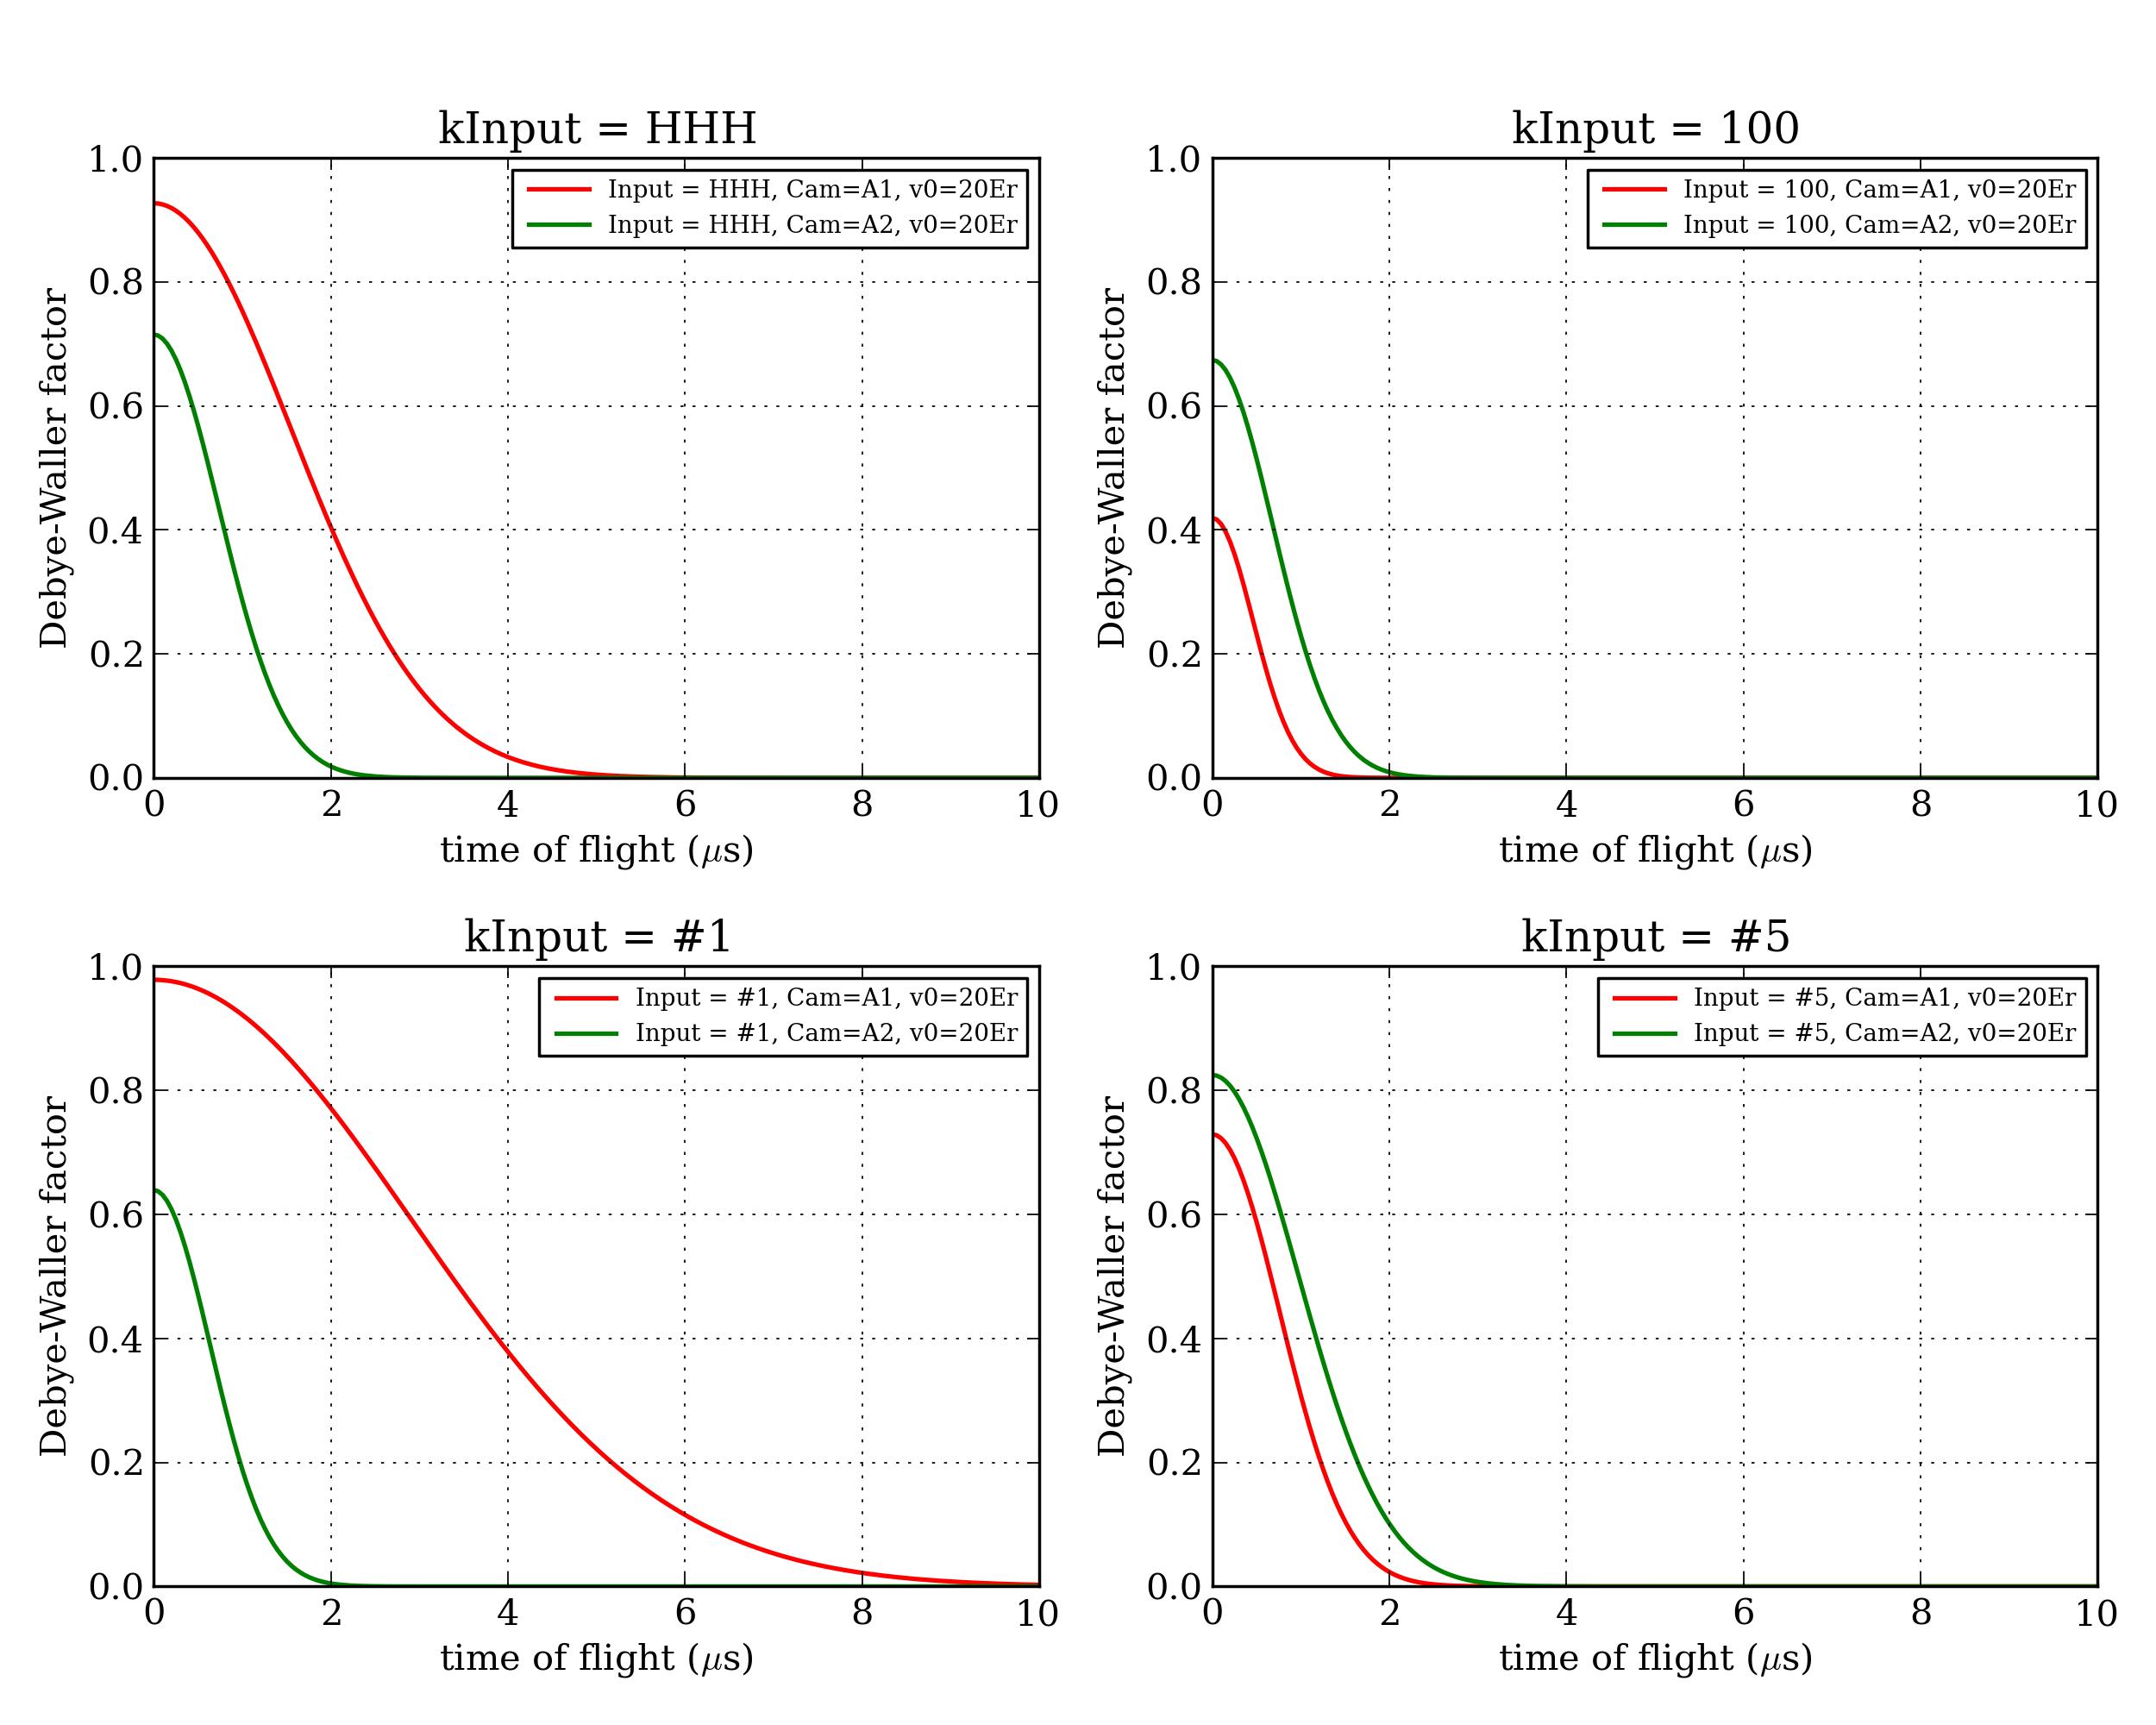
\includegraphics[width=\textwidth]{../debye-waller_HHH/DWtof_plot_20Er.png}
%%%\caption[Debye-Waller vs. TOF]{\small Figure shows the Debye-Waller factor as a function of TOF for different momentum transfers. At $t=0$ the atoms are released from a 20 recoil lattice.}
%%%\label{fig:debye-waller_HHH_tof}
%%%\end{figure}
%%%
%%%\subsubsection{Saturation due to probe intensity} 
%%%
%%%We look at the saturation due to the probe intensity for a momentum transfer $\bv{Q}_{\mathrm{AF}}$ corresponding to the HHH Bragg scattering peak for antiferromagnetically ordered sample, see Fig.~\ref{fig:pbragg_HHH}. 
%%%\begin{figure}:
%%%\centering 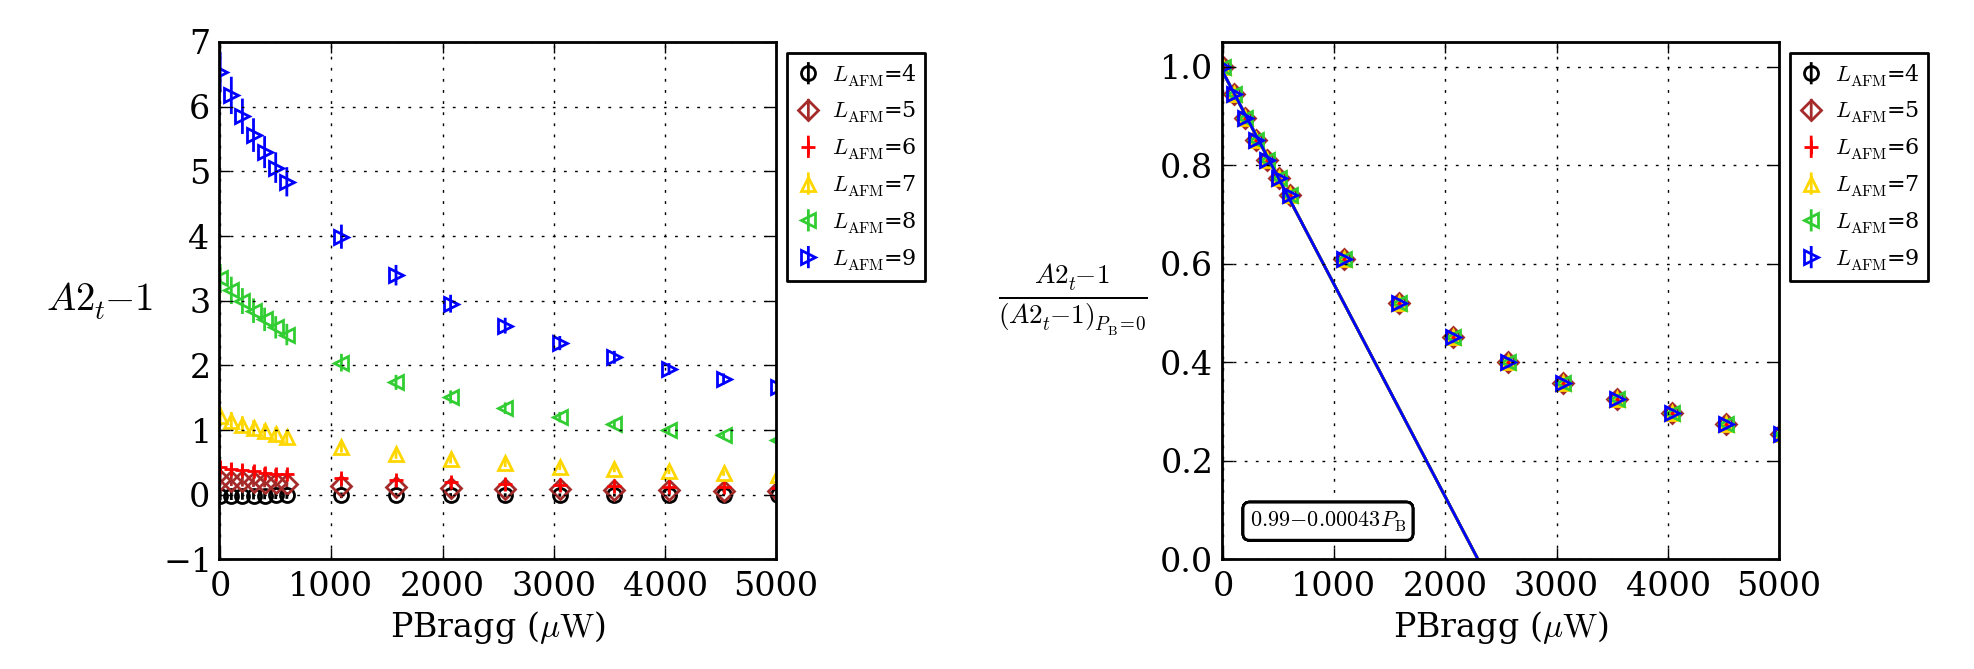
\includegraphics[width=\textwidth]{../pbragg_HHH/pbragg_HHH.png}
%%%\caption[Bragg vs. Power]{\small We use the abbreviation $\frac{X}{X_{\mathrm{TOF}}}=X_{t}$. Left panel shows the Bragg scattering
%%%intensity at camera $A2$ for a beam on the HHH input (Input \#3) as a
%%%function of probe power (Power translates into intensity given the known
%%%beam waist at the atoms). This corresponds to a momentum transfer equal
%%%to $\bv{Q}_{\mathrm{AF}}$.  The various sets correspond to different
%%%sizes of the AFM core used in the numerical evaluation.   Right panel
%%%shows the same as the left panel, but normalized to the value at zero
%%%power for each set.  All the sets collapse into one, and the dependency due to power at low powers is fitted to a straight line.} \label{fig:pbragg_HHH}
%%%\end{figure}
%%%In this case we find that for the power that we are using, $\approx 250
%%%\,\mu\mathrm{W}$,  the excess of counts at the Bragg camera $A2$, for an
%%%in-situ picture with respect to a TOF picture, are underestimated by $\approx$11\%.   
%%%
%%%At the moment we will carry on with the assumption that our measurement
%%%is in the low intensity regime, in this case we can go by
%%%Eq.~(\ref{eq:lowIntensityBragg}) to get the value of the spin structure
%%%factor since we know the value of the Debye-Waller factors for each of
%%%the momentum transfers that we measure.  Due to saturation effects then our value can be thought of as a lower bound to $S(\bv{Q})$.  In the future we are going to try to repeat the measurements with a lower Bragg power so that we do not run into this kind of issues.   
%%%
%%%\subsection{Estimating the size of the AFM domain}
%%%
%%%In our numerical evaluation of the scattered intensity we consider a lattice
%%%with an AFM domain in the center surrounded by a core with a random spin
%%%distribution.   This allows us to study the effect of the outside shell on our
%%%ability to see an AFM distribution in the core, see
%%%Fig.\ref{fig:braggCrystalSize}.
%%%\begin{figure}
%%%\centering 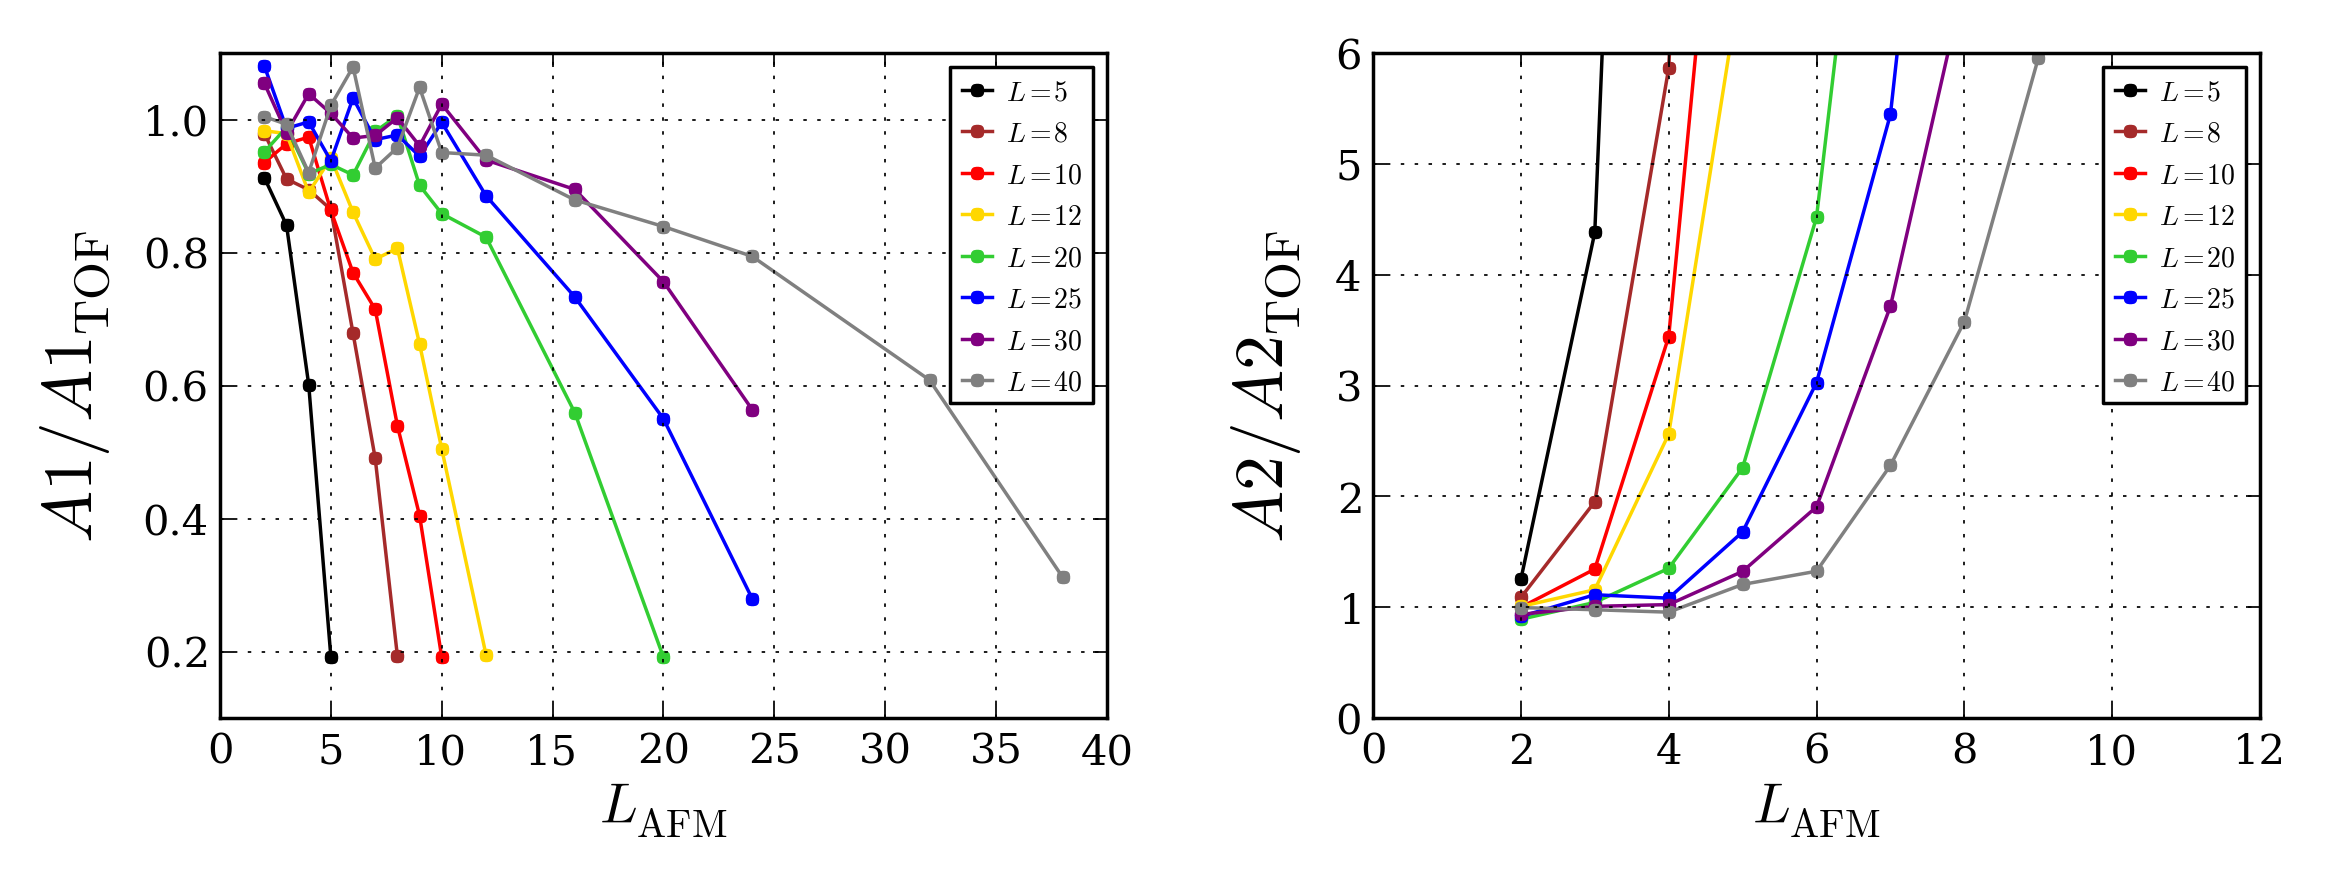
\includegraphics[width=\textwidth]{../crystalsize/CrystalSize.png}
%%%\caption[Bragg for different system sizes]{\small Left panel shows the intensity at camera $A1$ normalized to TOF for different system sizes and AFM core sizes.  Right panel shows the same for the $A2$ camera. }
%%%\label{fig:braggCrystalSize}
%%%\end{figure}
%%%   Our system size is approximately $L=40$,  and
%%%for this size the Bragg signals that we obtain $A2_{\mathrm{t}}\approx1.25$ (we
%%%have seen up to 1.5 sometimes) would be consistent with an AFM core size of
%%%approximately $6^{3}$ sites.  On the other hand we also see a depletion on camera $A1$ of $A1_{t}\approx0.75$, which would be consistent with an AFM core of $25^{3}$ lattice sites.   We believe that our model is not really good for this kind of estimates and this is more the realm of the QMC people, in any case we show what we obtain.  
%%%
%%% 
%%%%\subsection{ Analytical dependence of crystal and magnetic structure factors
%%%%on \bv{Q}}
%%%%
%%%%\subsubsection{Crystal}
%%%%
%%%%\begin{equation}
%%%%C(\bv{Q}) = \sum_{jk} e^{i \bv{Q} \cdot (\bv{R}_{j} - \bv{R}_{k} )} 
%%%%\end{equation}
%%%%
%%%%We can make the substitution $\bv{r}_{k} = \bv{R}_{j} -
%%%%\bv{R}_{k}$.  For an infinite crystal, the sum over all pairs $jk$ may be replaced by the sum over all
%%%%sites $j$ and then sum over all $\bv{r}_{k}$.
%%%% 
%%%%\begin{equation}
%%%%C(\bv{Q}) = N\sum_{k} e^{i \bv{Q} \cdot \bv{r}_{k}} 
%%%%\end{equation}
%%%%
%%%%\subsubsection{Magnetic}
%%%%
%%%%\begin{equation}
%%%%S(\bv{Q}) = \sum_{jk} e^{i \bv{Q} \cdot (\bv{R}_{j} - \bv{R}_{k} )} \langle S_{zj} S_{zk} \rangle
%%%%\end{equation}
%%%%
%%%%In the zero temperature AFM state there is a staggered magnetization, such that 
%%%%
%%%%\begin{equation}
%%%%\langle S_{zj}S_{zk} \rangle = e^{i \bv{q} \cdot (\bv{R}_{j} - \bv{R}_{k} )} 
%%%%\ \ \ \mathrm{where} \ \ \  
%%%%\bv{q} = \frac{2\pi}{a} \left( \frac{1}{2}\, \frac{1}{2}\, \frac{1}{2} \right)
%%%%\end{equation}
%%%%
%%%%At finite temperature, the staggered magnetization will have a finite correlation length \Lc, which results in 
%%%%
%%%%\begin{equation}
%%%%\langle S_{zj}S_{zk} \rangle = e^{i \bv{q} \cdot (\bv{R}_{j} - \bv{R}_{k} )} e^{-|\bv{R}_{j} -\bv{R}_{k} |/ \Lc }
%%%% \ \ \ \mathrm{where} \ \ \   
%%%%\bv{q} = \frac{2\pi}{a} \left( \frac{1}{2}\, \frac{1}{2}\, \frac{1}{2} \right)
%%%%\end{equation}
%%%%
%%%%\begin{equation}
%%%%S(\bv{Q}) = \sum_{jk} e^{i (\bv{Q} + \bv{q} )\cdot (\bv{R}_{j} - \bv{R}_{k} )} e^{-|\bv{R}_{j} -\bv{R}_{k} |/ \Lc }
%%%%\end{equation}
%%%%
%%%%At this point we can make the substitution $\bv{r}_{k} = \bv{R}_{j} -
%%%%\bv{R}_{k}$.  For an infinite crystal, the sum over all pairs $jk$ may be replaced by the sum over all
%%%%sites $j$ and then sum over all $\bv{r}_{k}$. 
%%%%
%%%%\begin{equation}
%%%%S(\bv{Q}) = \sum_{jk} e^{i (\bv{Q} + \bv{q} )\cdot \bv{r}_{k} } e^{-r_{k}/ \Lc } = N \sum_{k} e^{i (\bv{Q} + \bv{q} )\cdot \bv{r}_{k} } e^{-r_{k}/ \Lc }
%%%%\end{equation}

\bibliographystyle{osa}
\bibliography{bragg}

\end{document}




